\documentclass[14pt,candidate,times,fixint=false]{disser}

\usepackage[a4paper,pdftex,nohead,includefoot,
  left=3.5cm,right=1.8cm,top=2.0cm,bottom=1.7cm,footskip=1.3cm]{geometry}
\usepackage{ucs}
\usepackage[T2A]{fontenc}
\usepackage[utf8]{inputenc}
\usepackage[english,russian]{babel}
\usepackage{feynmf}
\usepackage{colortbl}
\usepackage{xspace}
\usepackage{maybemath}

\unitlength=1mm
\providecommand{\No}{\textnumero}
\graphicspath{{figures1/}{figures2/}{figures3/}{figures4/}}
\PrerenderUnicode{ая}

\pdfinfo{
  /Title (Musinsky Jan - Ph.D. dissertation)
  /Author (Jan Musinsky)
  /Subject (Ph.D. dissertation)
  /Keywords (charge exchange;drift chambers)
  /CreationDate (D:20090624120000)
}

\newcommand{\np}{\ensuremath{np \rightarrow pn}\xspace}
\newcommand{\dpfrag}{\ensuremath{dp \rightarrow ppn}\xspace}
\newcommand{\dpret}{\ensuremath{dp \rightarrow (pn)p}\xspace}
\newcommand{\dpchex}{\ensuremath{dp \rightarrow (pp)n}\xspace}
\newcommand{\dpela}{\ensuremath{dp \rightarrow dp}\xspace}
\setcounter{tocdepth}{2}

\begin{document}
\institution{
  \vspace{6ex}
  
\includegraphics[width=4.0cm]{jinr_logo.pdf} \\
  ОБЪЕДИНЁННЫЙ ИНСТИТУТ ЯДЕРНЫХ ИССЛЕДОВАНИЙ}
\topic{Исследование зарядово-обменных процессов \\
  в дейтрон-протонных взаимодействиях}
\author{МУШИНСКИ Ян}
\specnum{01.04.16}
\spec{Физика атомного ядра и элементарных частиц}
\title{Диссертация на соискание учёной степени \\
  кандидата физико-математических наук}
\sa{Глаголев~В.~В.}
\sastatus{д.~ф.-м.~н.,~проф.}
\city{Дубна}
\date{2010 \vspace{4ex}}
\maketitle

%%% Local Variables:
%%% mode: latex
%%% TeX-master: "musinsky_disser"
%%% coding: utf-8
%%% End:

\tableofcontents
\intro
В последние годы, вместе с развитием техники эксперимента, появилась реальная
возможность осуществления исследований, использующих поляризованные пучки и
мишени в ускорительных центрах мира. Возникла так называемая спиновая физика,
задачами которой стали решения классических задач ядерной и субъядерной физики,
интерес к которым давно возбуждался теоретиками.

Состояния систем тождественных частиц описываются волновыми функциями, которые
являются либо симметричными, либо антисимметричными при перестановке любой пары
частиц. В квантовой механике доказывается, что симметрия функций системы частиц
остаётся неизменной в любой момент времени. Частицы обладающие полуцелым спином
и подчиняющиеся статистике Ферми"--~Дирака, описываемые антисимметричными
волновыми функциями, подчиняются принципу Паули, запрещающему в данной системе в
одном и том же квантовом состоянии находиться более чем одному фермиону. В
данной работе рассматривается простейшая система двух нуклонов~--- дейтрон. В
соответствии с выше сказанным, волновая функция этой системы обладает свойствами
антисимметрии.

Дейтрон является слабосвязанной системой из нейтрона и протона. Спин дейтрона
равен единице, энергия связи 2.23 МэВ. Вследствие малой энергии связи, импульсы
внутриядерного Ферми движения нуклонов также являются небольшими (порядка 50
МэВ/с) и при больших энергиях падающих на дейтрон частиц слабо влияют на
квазинуклонное взаимодействие с протоном или нейтроном ядра. Это позволяет
применять к рассмотрению взаимодействий на дейтроне так называемое импульсное
приближение.

При взаимодействиях высокоэнергичных частиц с дейтроном заметно выделяется класс
вторичных частиц, называемых спектаторами, относительно которых принимается, что
они являются как бы <<наблюдателями>> при квазинуклонном столкновении падающей
частицы с <<другим>> нуклоном дейтрона. На практике импульсные распределения
спектаторов хорошо описываются с помощью известных волновых функций дейтрона,
что подтверждает применимость импульсного приближения. В случае малых
передаваемых импульсов при взаимодействии разумно предполагать, что квантовые
состояния спектаторов и нуклонов отдачи сохраняются такими же, какими они были
в составе дейтрона. Это особенно отчётливо проявляется в случае обратной
кинематики, когда ядро (в данном случае дейтрон) падает на протон.

В теории нуклон-нуклонного рассеяния, фундаментальное значение имеет извлечение
(восстановление) комплексных амплитуд матрицы рассеяния. Для получения всех
амплитуд необходимо проводить так называемый полный опыт, в результате которого
должен быть получен такой набор экспериментальных наблюдаемых, который позволяет
провести исчерпывающее описание процесса. Полный эксперимент включает в себя
измерения с поляризованными частицами-снарядами, а также с поляризованными
мишенями. Это весьма большая и трудоёмкая задача.

Однако, в некоторых случаях возможно определить отдельные амплитуды матрицы
рассеяния, либо их совокупность, путём выбора некоторых экспериментальных
условий. Одной из возможностей является изучение реакции перезарядки на
дейтроне, которая \! при некоторых условиях определяется только зависящими от
спина компонентами амплитуд. Таких ограничений не возникает для перезарядки на
свободном нуклоне. Эта идея была формализована математически в целом ряде
теоретических работ. Важно то, что появилась возможность извлечь спин-зависящую
часть амплитуды $np$-рассеяния с использованием неполяризованных протонов и
неполяризованных дейтронов в реакциях перезарядки на дейтроне. Экспериментально
такую серию работ пытались решать в основном, в пучках сепарированных нейтронов
и, в последствии, в квази-монохроматических нейтронах от стриппинга ускоренных
дейтронов.

Мы сочли целесообразным провести анализ \! экспериментальных данных, в которых
ускоренные дейтроны падали на протонную мишень. При такой постановке опыта
дейтроны монохроматичны, а вторичные два протона~--- продукты перезарядки
дейтрона на протоне, являются быстрыми и вылетают в переднем направлении под
малыми углами. Такой эксперимент был проведён на синхрофазотроне ЛВЭ ОИЯИ с
использованием в качестве одновременно детектора и мишени водородной пузырьковой
камеры. До начала наших исследований другие эксперименты с пучком дейтронов
практически отсутствовали.

Анализ экспериментальных данных оправдал наши надежды и кроме того, по мере
развития детектирующей техники и систем сбора данных, позволил сформулировать
требования к решению задачи электронными методами. Была создана установка
СТРЕЛА, которая начала функционировать на пучке дейтронов, ускоренных на
Нуклотроне ЛФВЭ ОИЯИ.

Из вышесказанного видно, что тема диссертации является актуальной. Целью
диссертационной работы является:
\begin{itemize}
\item Проведение полного анализа реакции перезарядки в дейтрон-протонных
  взаимодействиях на водородной пузырьковой камере для определения
  спин-зависящей части амплитуды $np$-рассеяния.
\item Предложение на основе этого анализа постановки эксперимента с
  использованием современной электронной методики и обоснование выбора геометрии
  эксперимента.
\item Испытание всех элементов установки СТРЕЛА, в том числе дрейфовых камер в
  качестве трековых приборов высокой разрешающей способности.
\item Создание систем программного обеспечения во время облучения установки и
  восстановления треков в дрейфовых камерах.
\end{itemize}

В настоящей работе приведены результаты физических и методических исследований
по теме диссертации. Она состоит из введения, четырёх глав, заключения и списка
цитируемой литературы. Во введении кратко обсуждаются предпосылки постановки
задачи.

Первая глава диссертации посвящена истории вопроса, теоретическому формализму
основной идеи эксперимента, а также результатам исследования элементарной
реакции \np перезарядки в различных экспериментах.

Вторая глава содержит результаты анализа реакции перезарядки в дейтрон-протонных
взаимодействиях полученных на жидководородной пузырьковой камере. С помощью
измерения дифференциального поперечного сечения реакции перезарядки \dpchex
оценён вклад спин-зависящей амплитуды \np рассеяния.

В третьей главе сформулировано предложение нового электронного эксперимента и
подробно описывается установка СТРЕЛА. Обсуждается структура установки и её
основные элементы. Внимание уделено дрейфовым камерам, являющимся основными
составляющими установки.

Четвёртая глава посвящена процедуре восстановления треков и соответствующему
программному обеспечению. В заключении сформулированы основные результаты
диссертационной работы. Список цитируемой литературы включает ссылки на
92 работу по теме диссертации.

Анализ экспериментальных данных и результаты методических исследований,
включённые в диссертацию, опубликованы в виде статей в научной периодике, а
также докладывались на ряде международных конференций и семинаров. В том числе,
на международных совещаниях «Релятивистская ядерная физика: от сотен МэВ до ТэВ»
в Стара Лесна (Словакия~--- 2000 и 2009~г.) и Модра Гармония (Словакия~---
2006~г.), на рабочем совещании по протон-дейтронным взаимодействиям (Дубна~---
2002~г.), на международном семинаре по проблемам физики высоких энергий
<<Релятивистская ядерная физика и квантовая хромодинамика>> (Дубна~--- 2000,
2002 и 2006~г.) и на семинарах ЛФВЭ ОИЯИ. Список публикаций, на которых основана
диссертация, содержит 12 наименований.

%%% Local Variables:
%%% mode: latex
%%% TeX-master: "musinsky_disser"
%%% coding: utf-8
%%% End:

\chapter{Дейтрон-протонные взаимодействия
  с перезарядкой}
В конце 1950 года на собрании Американского физического общества в
Калифорнийском Университете состоялся доклад Кладиса и его
группы~\cite{cladis50}, в котором обсуждались результаты облучения ядер дейтерия
нейтронным пучком с энергией 270 МэВ. Данные этого эксперимента были получены
на ускорителе в Беркли (США) и позднее опубликованы в
работах~\cite{cladis52,moyer52}. В докладе отмечалось, что выход быстрых
вторичных протонов (с приблизительно такой же энергией, как энергия падающих
нейтронов) в $nd$-рассеянии, в направлении падающих нейтронов, был подавлен
относительно их выхода в $np$-рассеянии в согласии с принципом Паули для двух
нейтронов с малыми относительными импульсами в реакциях с обменом заряда.

Данное экспериментальное наблюдение дало начало более детальным теоретическим
рассмотрениям, которые продолжаются и по сей день. Одним из первых в 1951 году
опубликовал свою работу Померанчук~\cite{pom51}.  В ней он указал на
возможность выяснения зависимости обменных сил от спина из сравнения процессов
рассеяния нуклонов на дейтроне с упругим рассеянием нейтрона на протоне, в
случае, когда нейтрон и протон обмениваются между собой зарядом (перезарядка). В
конце того же года, практически одновременно и независимо, с аналогичным
предложением выступил и Чу~\cite{chew51}, рассматривавший неупругое рассеяние
нейтронов на дейтроне при энергиях 90 МэВ.

Об изменении (повороте) спина одного из нуклонов в процессе $np$-перезарядки
говорилось и в работе Мигдала~\cite{mig55}. В 1957 году вышла работа
Лапидуса~\cite{lap57}, в которой обсуждалась теория обменных столкновений
быстрых нуклонов с дейтронами. В ней было показано, что сопоставление
экспериментальных данных об обменном рассеянии быстрых нуклонов дейтронами с
расчётами в импульсном приближении помогает фазовому анализу данных об
$np$-рассеянии. Автор при этом опирался на экспериментальные данные, полученные
группой Джелепова при энергиях от 380 по 590 МэВ на синхроциклотроне ИЯП АН
СССР, теперь ЛЯП ОИЯИ (измерения происходили в 1952--1954 годах, ещё до
основания Объединённого института ядерных
исследований)~\cite{dzelep56,dzelep58}.

В дальнейшем наиболее чёткая теоретическая формулировка для проведения оценки
вкладов спин-зависящей и спин-независящей частей амплитуды $np$-рассеяния из
процесса перезарядки на дейтроне была представлена в работах
Дина~\cite{dean72,dean72_2}. Полученные им формулы, выведенные в импульсном
приближении, используются во многих работах до последнего времени. Заметный
вклад в теоретический формализм и интерпретацию экспериментальных данных внесли
тоже Багг, Вилкин, Легар и другие известные учёные, теоретики.

Рассмотрим в простейшем виде два процесса, схематически изображённые на
рис.~\ref{fig:np_dp_scheme}, т.е. элементарную реакцию перезарядки нейтрона на
протоне \np и реакцию перезарядки дейтрона на протоне-мишени \dpchex. Здесь в
скобках два протона, связанные с падающим дейтроном, а именно,
протон-спектатор и протон от квази \np перезарядки, т.е. перезарядки
нейтрона (связанного в дейтроне) на протоне-мишени. Вертикальными стрелками
обозначены направления спинов нуклонов относительно произвольной оси
квантования. В первом случае, реакция \np на рис.~\ref{fig:np_dp_scheme}~а),
возможны оба направления спина рассеянного протона. Для второго случая, реакция
\dpchex на рис.~\ref{fig:np_dp_scheme}~б), при рассеянии на малый угол
(пространственная симметрия) в силу возникшей зарядовой симметрии (два протона
вылетают вперёд с малым относительным импульсом) процесс в силу принципа Паули
(статистика Ферми"--~Дирака для полуцелых спинов) может идти только с
переворотом спина у рассеянного протона. Дейтрон в данном случае выступает как
<<спиновый фильтр>>.

\begin{figure}[h]
  \centering
  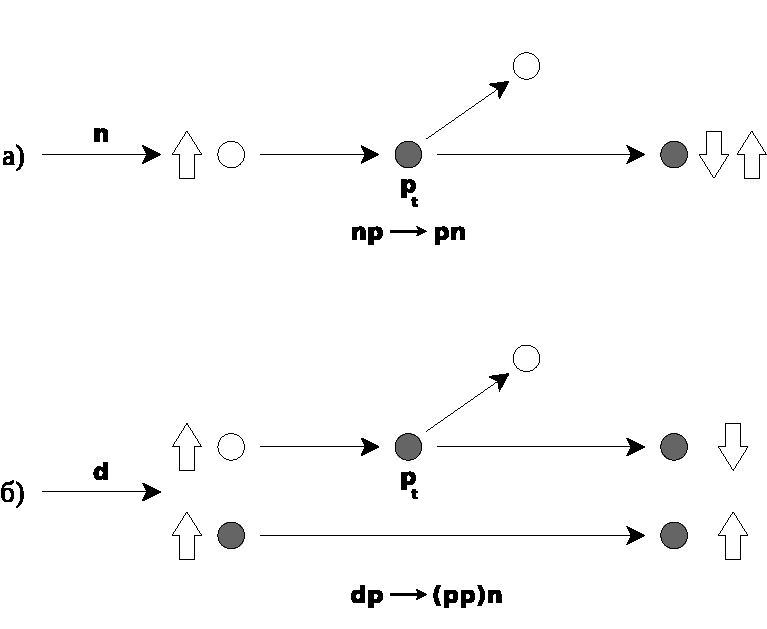
\includegraphics[width=0.85\textwidth]{np_dp_scheme.pdf}
  \caption{Схематическое изображение а) элементарной реакции перезарядки \np
    и б) перезарядки дейтрона на протоне-мишени \dpchex. Пустые кружки
    представляют нейтрон а сплошные протон, $p_{t}$~--- протон-мишени,
    вертикальные стрелки~--- направления спинов нуклонов.}
  \label{fig:np_dp_scheme}
\end{figure}

Возможность использования реакции перезарядки на дейтроне для получения
информации о спиновой зависимости реакции перезарядки \np качественно можно
объяснить следующим образом. Два нуклона~--- протон и нейтрон, связанные в
дейтроне, могут находиться в состояниях $^3S_1$ и $^3D_1$ (изоспин $I=0$)
симметричных по пространственным и спиновым переменным, но одновременно
антисимметричных по зарядовой переменной. В процессе перезарядки дейтрона на
протоне, когда образуется симметричная по заряду система из двух протонов, в
силу принципа Паули при сохранении пространственной симметрии, асимметрия полной
волновой функции дейтрона будет обеспечена переворотом спина рассеянного нуклона
(состояния $^1S_0$ или $^1D_2$ для пары протонов). Таким образом, спин-зависящая
часть амплитуды элементарной $np$-перезарядки будет проявляться через
вероятность реакции перезарядки на дейтроне~\cite{gla_mucha00}.

\section{Теоретический формализм}
\label{section:theory}
Наиболее прямым феноменологическим способом описания процесса рассеяния двух
нуклонов является определение (получение) соответствующих элементов матрицы
рассеяния непосредственно по экспериментальным данным. В описании матрицы будем
опираться на представления амплитуд нуклон-нуклонного рассеяния
Гольдбергера"--~Ватсона~\cite{gold66}. Заметим, что во многих других работах
часто используется и представление Быстрицкого, Легара,
Винтерница~\cite{bys78_2}. Оба представления амплитуд матрицы рассеяния
равнозначны и дают одинаковые результаты.

Для теоретического описания процесса нуклон-нуклонного рассеяния удобно
использовать систему центра масс с базисными векторами $(\mathbf{l, m, n})$,
определяющими ортонормированную систему координат, связанную с налетающей
частицей, где
\begin{equation}
  \label{eq:ort}
  \mathbf{l} =
  \frac{\mathbf{p}_f + \mathbf{p}_i}{|\mathbf{p}_f + \mathbf{p}_i|}\,, \qquad
  \mathbf{m} =
  \frac{\mathbf{p}_f - \mathbf{p}_i}{|\mathbf{p}_f - \mathbf{p}_i|}\,, \qquad
  \mathbf{n} =
  \frac{\mathbf{p}_i \times \mathbf{p}_f}{|\mathbf{p}_i \times \mathbf{p}_f|}\,.
\end{equation}
Векторы импульса налетающего и рассеянного нуклона обозначены $\mathbf{p}_i$ и
$\mathbf{p}_f$, соответственно. Ось базисного вектора $\mathbf{n}$
перпендикулярна к плоскости рассеяния, определённой векторами импульсов
налетающего $\mathbf{p}_i$ и рассеянного $\mathbf{p}_f$ нуклона.

В общем виде, матрицу рассеяния $T$, феноменологически описывающую процесс
$NN$-рассеяния, можно записать с помощью линейных функций $A$ и $B$, зависимых
от $\boldsymbol{\sigma}_1$ и трёх ортогональных векторов, определённых
выражением~\eqref{eq:ort}, в виде
\begin{equation}
  \label{eq:mat}
  T = A + B\,\boldsymbol{\sigma}_2\,,
\end{equation}
где $\boldsymbol{\sigma}_1$ и $\boldsymbol{\sigma}_2$~--- $2 \times 2$-спиновые
матрицы Паули действующие на волновую функцию налетающего нуклона и
нуклона-мишени. При разложении функций $A$ и $B$ по объединённому спиновому
пространству обоих нуклонов матрица рассеяния~\eqref{eq:mat} имеет следующий
общий вид
\begin{equation}
  \label{eq:mat_full}
  \begin{split}
    T = \ &\ a_1 +
    a_2(\boldsymbol{\sigma}_1\cdot\mathbf{l}) +
    a_3(\boldsymbol{\sigma}_1\cdot\mathbf{m}) +
    a_4(\boldsymbol{\sigma}_1\cdot\mathbf{n})\ + \\
    +\ &\bigl[b_1 +
    b_2(\boldsymbol{\sigma}_1\cdot\mathbf{l}) +
    b_3(\boldsymbol{\sigma}_1\cdot\mathbf{m}) +
    b_4(\boldsymbol{\sigma}_1\cdot\mathbf{n})\bigr]
    \,(\boldsymbol{\sigma}_2\cdot\mathbf{l})\ + \\
    +\ &\bigl[c_1 +
    c_2(\boldsymbol{\sigma}_1\cdot\mathbf{l})\,+
    c_3(\boldsymbol{\sigma}_1\cdot\mathbf{m}) +
    c_4(\boldsymbol{\sigma}_1\cdot\mathbf{n})\bigr]
    \,(\boldsymbol{\sigma}_2\cdot\mathbf{m})\ +\\
    +\ &\bigl[d_1 +
    d_2(\boldsymbol{\sigma}_1\cdot\mathbf{l}) +
    d_3(\boldsymbol{\sigma}_1\cdot\mathbf{m}) +
    d_4(\boldsymbol{\sigma}_1\cdot\mathbf{n})\bigr]
    \,(\boldsymbol{\sigma}_2\cdot\mathbf{n})\,,
  \end{split}
\end{equation}
где коэффициенты $a_i, b_i, c_i$ и $d_i$ относятся к комплексным амплитудам
нуклон-нуклонного рассеяния. Спиновая матрица размером
$4 \times 4$~\eqref{eq:mat_full} полностью описывает всю динамику процесса
рассеяния двух нуклонов.

Следуя работе~\cite{gold66}, все 16 матричных элементов можно выразить через 5
амплитуд рассеяния, если наложить требования пространственной и временной
инвариантности, а также предполагать зарядовую симметрию ядерных сил. Такие
предположения позволяют представить общий вид матрицы рассеяния $T$ в упрощённой
форме
\begin{equation}
  \label{eq:mat_final}
  \begin{split}
    T =\ &a\ +\ b
    (\boldsymbol{\sigma}_1\cdot\mathbf{n})
    (\boldsymbol{\sigma}_2\cdot\mathbf{n})\ +\ c\bigl[
    (\boldsymbol{\sigma}_1\cdot\mathbf{n}) +
    (\boldsymbol{\sigma}_2\cdot\mathbf{n})\bigr]\ \ +\\
    +\ &e
    (\boldsymbol{\sigma}_1\cdot\mathbf{m})
    (\boldsymbol{\sigma}_2\cdot\mathbf{m})\ +\ f
    (\boldsymbol{\sigma}_1\cdot\mathbf{l})
    (\boldsymbol{\sigma}_2\cdot\mathbf{l})\,.
  \end{split}
\end{equation}
Комплексные амплитуды $a, b, c, e$ и $f$ являются функциями энергии реакции и
угла рассеяния взаимодействующих частиц. Таким образом, нуклон-нуклонное
рассеяние в общем виде полностью описывается всего пятью комплексными
амплитудами. Из уравнения~\eqref{eq:mat_final} видно, что только первый член
матрицы рассеяния $T$, комплексная амплитуда $a$, не зависит от спина.

Дифференциальное поперечное сечение \np рассеяния, следуя работе~\cite{bys78_2},
можно записать как
\begin{equation}
  (d\sigma/dt)_{\np} = (\pi/p^2)\,
  \bigl[\,|a|^2 + |b|^2 + 2|c|^2 + |e|^2 + |f|^2 \bigr]
\end{equation}
и может быть представлено в виде суммы спин-независящей (индекс $SI$) и
спин-зависящей (индекс $SD$) частей
\begin{equation}
  (d\sigma/dt)_{\np} = (d\sigma/dt)^{SI}_{\np} + (d\sigma/dt)^{SD}_{\np}\,,
\end{equation}
где $p$~--- импульс с системе центра масс двух нуклонов, а $t$~--- квадрат
четырёхмерного переданного импульса. Для отдельных частей дифференциального
сечения получаем
\begin{align}
  (d\sigma/dt)^{SI}_{\np} &= (\pi/p^2)\,|a|^2\,,\\
  \label{eq:np_SD}
  (d\sigma/dt)^{SD}_{\np} &= (\pi/p^2)\,
  \bigl[\,|b|^2 + 2|c|^2 + |e|^2 + |f|^2\bigr]\,.
\end{align}

Математический формализм, который в рамках импульсного приближения позволяет
записать дифференциальное поперечное сечение реакции перезарядки на дейтроне
через дифференциальное поперечное сечение элементарной реакции перезарядки
на нуклоне, обсуждался во многих работах~\cite{dean72,dean72_2,bugg87}.
В импульсном приближении, амплитуда рассеяния нуклонов сложным ядром (дейтроном)
представляется в виде суммы амплитуд рассеяния свободными нуклонами, имеющими
распределение импульсов, соответствующее в данный момент распределению импульсов
нуклонов в ядре~\cite{chew50,chew52}. Рассеяние падающей частицы на ядре можно
потом приблизительно рассматривать, как происходящее на отдельных нуклонах, так
как энергия связи частиц в ядре играет второстепенную роль, особенно в случае
дейтрона.

Соотношение между дифференциальными поперечными сечениями перезарядки дейтрона
на протоне \dpchex и элементарной перезарядкой \np при применении импульсного
приближения можно записать~\cite{dean72_2} как
\begin{equation}
  (d\sigma/dt)_{\dpchex} = \bigl[1 - F_d(t)\bigr]\,(d\sigma/dt)^{SI}_{\np} +\,
  \bigl[1 - 1/3\,F_d(t)\bigr]\,(d\sigma/dt)^{SD}_{\np}\,,
\end{equation}
где $F_d(t)$ обозначает формфактор дейтрона. Из этой формулы следует, что при
нулевой передаче импульса $(t=0)$, из-за того, что $F_d(0) = 1$,
дифференциальное поперечное сечение будет иметь следующий вид
\begin{equation}
  \label{eq:dp_23np}
  (d\sigma/dt)_{\dpchex} = 2/3\,(d\sigma/dt)^{SD}_{\np}\,.
\end{equation}

Таким образом, появилась возможность определения части взаимодействия нейтрона и
протона, которая полностью зависит от спина, из экспериментального анализа
дифференциального сечения реакции перезарядки дейтрона на протоне \dpchex ,
используя данные по перезарядке в элементарном процессе \np на неполяризованном
пучке и неполяризованном протоне-мишени.

Мы рассматриваем случай рассеяния назад, когда угол двух рассеявшихся нуклонов
(нейтрона и протона) близок к 180$^{\,\circ}$. При этих условиях вектор импульса
налетающего нуклона антипараллелен вектору импульса рассеянного нуклона
$(\mathbf{p}_i = -\,\mathbf{p}_f)$, а для амплитуд рассеяния выполняется
соотношение $b(\pi) = f(\pi)$ и $c(\pi) = 0$.  В итоге, следуя
уравнениям~\eqref{eq:np_SD} и~\eqref{eq:dp_23np}, для дифференциального
поперечного сечения \np рассеяния назад получаем простое выражение
\begin{equation}
  (d\sigma/dt)_{\dpchex} = 2/3\,(d\sigma/dt)^{SD}_{\np} =
  2/3\,(\pi/p^2)\,\bigl[\,2\,|b|^2 + |e|^2\bigr]\,.
\end{equation}
Изучение процесса перезарядки \dpchex при нулевых переданных импульсах позволяет
оценить спин-зависящую часть сечения элементарной реакции перезарядки \np,
которая определяется суммой всего двух амплитуд $2\,|b|^2 + |e|^2$.

\section{Сечение реакции перезарядки \maybebm{{\np}}}
\label{section:npnp}
Как видно из вышесказанного, для того, чтобы сделать оценку вклада
спин-зависящей части амплитуды \np рассеяния, используя данные по реакции
перезарядки на дейтроне, необходимо, кроме измерения дифференциального
поперечного сечения реакции \dpchex, иметь данные экспериментов по
дифференциальному сечению реакции элементарной перезарядки \np при $t=0$.
Из наших экспериментальных данных, которые были получены в пучке дейтронов
импульса 3.35~ГэВ/с, мы будем оценивать величину дифференциального поперечного
сечения для перезарядки на дейтроне при $t=0$ и сравниваем её с имеющимися в
литературе данными по этой величине для \np рассеяния при том же импульсе.

В работе Фридеса и др.~\cite{friedes65} проведённой в Брукхейвене (США) были
просуммированы данные по дифференциальному сечению реакции \np в диапазоне
импульсов нейтронов от 1.4 до 8.15~ГэВ/с и приведена полученная авторами
зависимость $d\sigma/dt\,|\,_{t=0}$ от импульса (более детальная информация об
этих измерениях отсутствует). Известна также работа Шепарда и др.~\cite{shep69},
позднее опубликованная в~\cite{shep74} по перезарядке в $np$-рассеянии в
диапазоне импульсов 600--2000 МэВ/с на протонном ускорителе в Принстоне (США).

Как и в других подобных экспериментах, пучок вторичных нейтронов формировался от
взаимодействий ускоренных протонов на внутренней мишени ускорителя. С помощью
магнитов, отклоняющих вторичные заряженные частицы, и коллиматоров пучок
нейтронов направлялся на жидководородную мишень. Выходящие из мишени в переднем
направлении быстрые протоны анализировались магнитным спектрометром.

Позднее на ускорителе Сатурн в Сакле (Франция) были проведены Бизардом и
др. систематические измерения дифференциальных сечений реакции перезарядки \np в
интересующем нас диапазоне импульсов нейтронов 1--2 ГэВ/с~\cite{biz75}. В
отличие от других аналогичных экспериментов, в этой работе использовались
квази-монохроматические нейтроны от стриппинга ускоренных дейтронов с импульсным
разбросом 5~$\%$.

Последний из нам известных экспериментов по $np$-рассеянию в интересующем нас
диапазоне энергий и с результатами по дифференциальному сечению при малых
значениях $t$ был выполнен в лаборатории Лос Аламос~(США) и опубликован в работе
Боннера и др.~\cite{bon78}.

На основе экспериментальных данных этих цитируемых работ, для каждого значения
импульса нейтрона в интервале от 1 до 2~ГэВ/с, строилась зависимость
дифференциального поперечного сечения $d\sigma/dt$ элементарной реакции
перезарядки \np от четырёхмерного переданного импульса $t$. На
рис.~\ref{fig:np_two_bizard} в качестве примера приведена такая зависимость для
двух разных импульсов налетающего нейтрона (измерения на ускорителе Сатурн при
импульсе 1.43 и 1.88 ГэВ/с).

\begin{figure}[h]
  \centering
  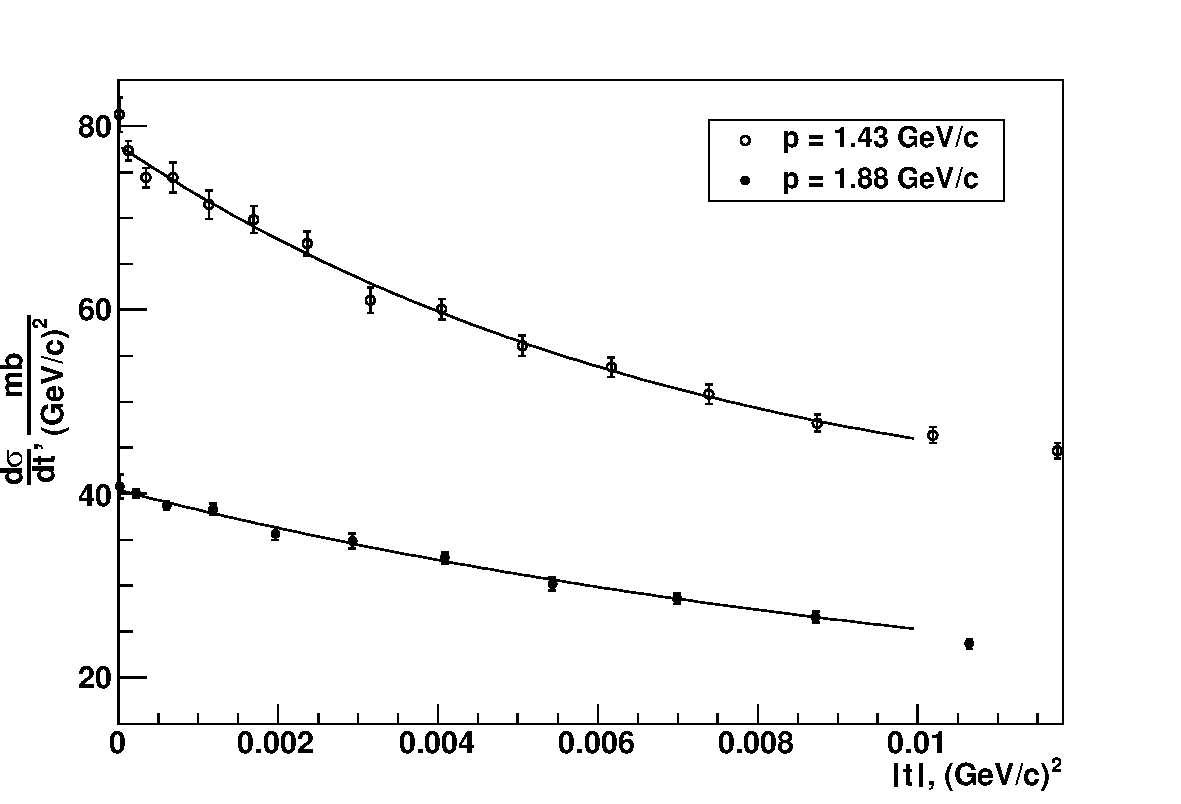
\includegraphics[width=1.00\textwidth]{np_two_bizard.pdf}
  \caption{Зависимость дифференциального поперечного сечения $d\sigma/dt$
    реакции перезарядки \np от четырёхмерного переданного импульса $t$ для двух
    разных импульсов $p$ налетающего нейтрона. Сплошные линии~--- аппроксимация
    экспериментальных данных функцией \eqref{eq:exp2}.}
  \label{fig:np_two_bizard}
\end{figure}

Индивидуальные сечения $d\sigma/dt$ при $t=0$ были получены путём аппроксимации
распределений $d\sigma/dt$ для каждого (всего~39) значения импульса нейтрона
выражением
\begin{equation} \label{eq:exp2}
  d\sigma/dt = p_0\exp(p_1\,t + p_2\,t^2)
\end{equation}
в интервале $t < 0.01$~(ГэВ/с)$^2$ и затем экстраполировались в точку $t=0$.
Полученные дифференциальные поперечные сечения $d\sigma/dt\,|\,_{t=0}$ реакции
перезарядки \np в интервале импульсов от 1 до 2~ГэВ/с приведены в
таблице~\ref{tab:np_data} и на рис.~\ref{fig:np_sigma0}.

\begin{table}[hp]
  \begin{center}
    \bigskip
    \resizebox{1.0\textwidth}{!} {
      \begin{tabular}{|c|c|c|}
        \hline $p$\,, & $d\sigma/dt\,|\,_{t=0}$\,, & Лаб. \\
        ГэВ/с & (ГэВ/с)$^2$ & \\ \hline \hline
        1.025 & 152.219 $\pm$ 0.873 & Лос Аламос \\ \hline
        1.033 & 156.199 $\pm$ 1.646 & Сакле \\ \hline
        1.045 & 144.949 $\pm$ 3.795 & Принстон \\ \hline
        1.055 & 142.571 $\pm$ 0.763 & Лос Аламос \\ \hline
        1.083 & 134.839 $\pm$ 1.310 & Сакле \\ \hline
        1.085 & 136.435 $\pm$ 0.571 & Лос Аламос \\ \hline
        1.115 & 129.173 $\pm$ 0.534 & Лос Аламос \\ \hline
        1.132 & 124.928 $\pm$ 1.150 & Сакле \\ \hline
        1.145 & 120.877 $\pm$ 0.594 & Лос Аламос \\ \hline
        1.146 & 114.784 $\pm$ 4.271 & Принстон \\ \hline
        1.175 & 115.738 $\pm$ 0.584 & Лос Аламос \\ \hline
        1.182 & 109.973 $\pm$ 0.958 & Сакле \\ \hline
        1.205 & 107.189 $\pm$ 0.650 & Лос Аламос \\ \hline
        1.232 & 105.913 $\pm$ 1.080 & Сакле \\ \hline
        1.235 & 101.102 $\pm$ 0.691 & Лос Аламос \\ \hline
        1.260 & 98.797 $\pm$ 0.750 & Лос Аламос \\ \hline
        1.281 & 74.825 $\pm$ 2.804 & Принстон \\ \hline
        1.281 & 86.811 $\pm$ 1.332 & Сакле \\ \hline
        1.295 & 92.099 $\pm$ 0.735 & Лос Аламос \\ \hline
        \multicolumn{3}{|r|}{{продолжение \dots}} \\ \hline
      \end{tabular}
      \quad
      \begin{tabular}{|c|c|c|}
        \hline $p$\,, & $d\sigma/dt\,|\,_{t=0}$\,, & Лаб. \\
        ГэВ/с & (ГэВ/с)$^2$ & \\ \hline \hline
        1.325 & 86.636 $\pm$ 0.687 & Лос Аламос \\ \hline
        1.331 & 87.610 $\pm$ 1.148 & Сакле \\ \hline
        1.355 & 85.586 $\pm$ 0.700 & Лос Аламос \\ \hline
        1.381 & 77.721 $\pm$ 0.721 & Сакле \\ \hline
        1.385 & 81.942 $\pm$ 0.612 & Лос Аламос \\ \hline
        1.429 & 73.384 $\pm$ 0.303 & Лос Аламос \\ \hline
        1.431 & 77.932 $\pm$ 0.694 & Сакле \\ \hline
        1.481 & 68.842 $\pm$ 0.699 & Сакле \\ \hline
        1.484 & 53.359 $\pm$ 2.384 & Принстон \\ \hline
        1.531 & 70.749 $\pm$ 0.983 & Сакле \\ \hline
        1.580 & 59.855 $\pm$ 1.235 & Сакле \\ \hline
        1.630 & 56.144 $\pm$ 1.172 & Сакле \\ \hline
        1.680 & 59.372 $\pm$ 0.846 & Сакле \\ \hline
        1.729 & 40.091 $\pm$ 1.962 & Принстон \\ \hline
        1.730 & 53.252 $\pm$ 0.584 & Сакле \\ \hline
        1.780 & 47.591 $\pm$ 0.434 & Сакле \\ \hline
        1.831 & 43.857 $\pm$ 0.401 & Сакле \\ \hline
        1.881 & 40.405 $\pm$ 0.391 & Сакле \\ \hline
        1.931 & 35.176 $\pm$ 0.507 & Сакле \\ \hline
        1.981 & 28.170 $\pm$ 0.675 & Сакле \\ \hline
      \end{tabular}
    }
    \bigskip
    \caption{Дифференциальные поперечные сечения $d\sigma/dt\,|\,_{t=0}$ для
      реакции элементарной перезарядки \np в интервале импульсов от 1 до 2
      ГэВ/с. Значения сечений получены на основе экспериментальных данных
      лабораторий Лос Аламоса~\cite{bon78}, Сакле~\cite{biz75} и Принстонского
      университета~\cite{shep74}.}
    \label{tab:np_data}
  \end{center}
\end{table}



%%% Local Variables:
%%% mode: latex
%%% TeX-master: "../musinsky_disser"
%%% coding: utf-8
%%% End:


\begin{figure}[h]
  \centering
  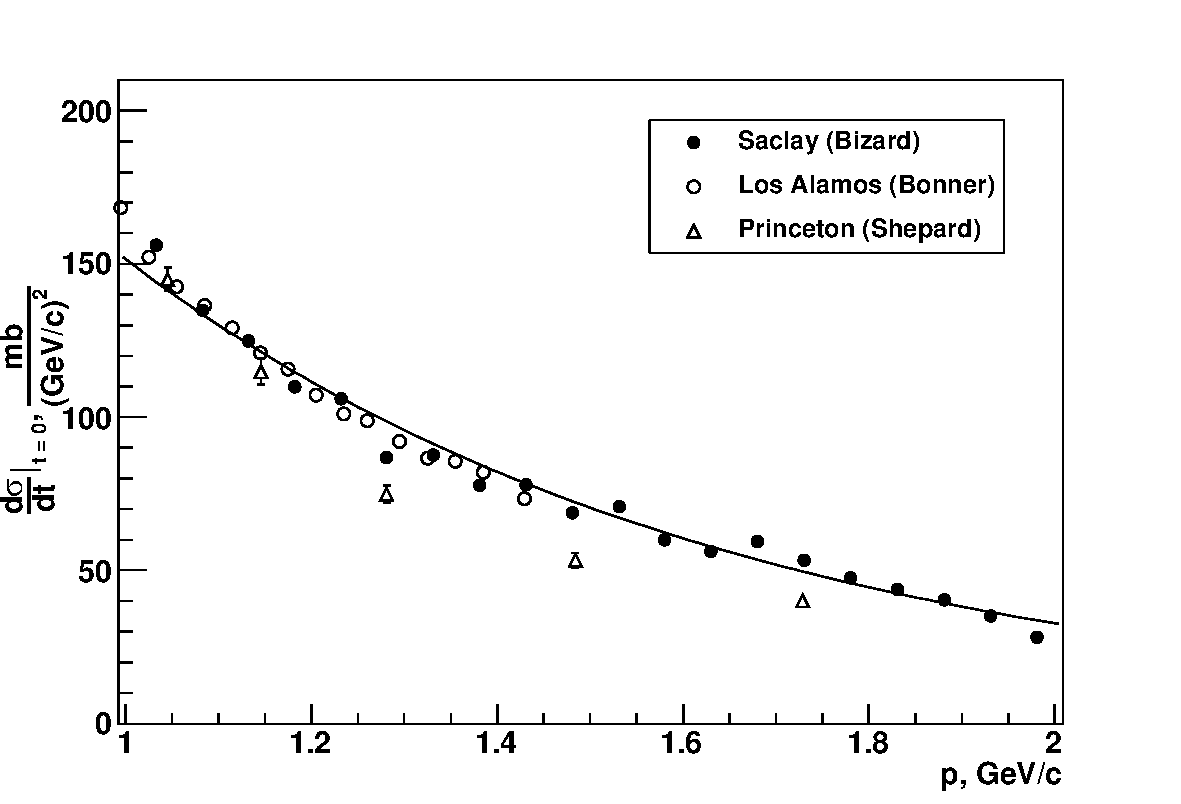
\includegraphics[width=1.00\textwidth]{np_sigma0.pdf}
  \caption{Зависимость дифференциального поперечного сечения
    $d\sigma/dt\,|\,_{t=0}$ элементарной реакции перезарядки \np от импульса $p$
    налетающего нейтрона. Сплошная линия~--- аппроксимация простой
    экспоненциальной функцией.}
  \label{fig:np_sigma0}
\end{figure}

Как видно, сечения перезарядки при $t=0$, полученные в Принстоне, оказались в
противоречии с данными других работ (были занижены примерно на 20~$\%$). Причина
такого расхождения неоднократно дискутировалась в научной периодике, но так и не
была объяснена. С другой стороны, данные полученные в Лос Аламосе очень близки к
данным Сакле. Поэтому считается, что измерения, проведённые Бизардом и др. на
ускорителе Сатурн в Сакле являются более корректными~\cite{biz75,bys78,nn_web}.
К тому же они проведены в интересующей нас области энергий 1 ГэВ и выше.

Зависимость, показанная на рис.~\ref{fig:np_sigma0}, была аппроксимирована
простой экспоненциальной функцией (аппроксимируются только данные получены
Бизардом и др.). В результате получаем выражение зависимости значения
$d\sigma/dt\,|\,_{t=0}$ реакции перезарядки \np от импульса $p$ налетающего
нейтрона
\begin{equation}
  \label{eq:np0}
  (d\sigma/dt\,|\,_{t=0})/p = 713.112 \exp(-1.533\,p)\,,
\end{equation}
которое будем в дальнейшем использовать.

Доступность результатов измерений, приведённых в работе Бизарда и др., дала
возможность проведения оценки спин-зависящей части амплитуды $np$-рассеяния при
их анализе совместно с результатами измерений дифференциальных сечений
перезарядки на дейтроне. Отметим, что опубликованные ранее данные~\cite{mucha02}
были сравнены с сечениями из работ Фридеса и
Шепарда~\cite{friedes65,shep69,shep74}, в которых значения
$d\sigma/dt\,|\,_{t=0}$ реакции перезарядки \np были, как было показано,
занижены.

\section{Избранные исследования с дейтронами}
В 80-х годах на синхрофазотроне ЛВЭ ОИЯИ были ускорены дейтроны, сначала с целью
получения вторичных нейтронных пучков от реакций стриппинга на бериллиевой
мишени. Был сформирован  канал в направлении на водородную камеру и в дальнейшем
она была экспонирована нейтронами нескольких энергий. Одновременно, используя
уже имевшийся канал для транспортировки заряженных частиц, камера облучалась
выведенным из ускорителя пучком дейтронов. Появилась возможность изучать
дейтрон-протонные взаимодействия с помощью водородной пузырьковой камеры в
условиях 4$\pi$-геометрии. Было получено большое количество результатов по
различным направлениям исследований и создана база данных, в частности, по
реакции перезарядки \dpchex. Результаты этого эксперимента будут обсуждены в
следующей главе диссертации.

Другой группой физиков (Струнов, Шаров) была создана установка
Дельта-Сигма~\cite{shar00}. На этой установке изучалась разница полных сечений
нейтрон-протонных взаимодействий  при двух различных направлениях продольной
поляризации падающего нейтрона и протона в поляризованной мишени. Позднее
установка была дополнена магнитным спектрометром для измерения импульсов
протонов из процессов $np$-перезарядки вылетающих в переднем направлении.

В этих работах использовались как жидководородная, так и жидкодейтериевая
мишени, что позволило в рамках одной геометрии эксперимента измерять
дифференциальные сечения как $np$, так и $nd$-процессов перезарядки. Авторам
удалось пройти в ранее неисследованную область энергий нейтронов выше
1~ГэВ. Мишень установки была окружена сцинтилляционными счётчиками работающими в
режиме антисовпадения с целью уменьшения фона от неупругих
процессов~\cite{shar04}.

Нам известно также об экспозиции водородной пузырьковой камеры в пучке
сепарированных дейтронов в KEK (Япония) в диапазоне импульсов
2.0--3.7~ГэВ/с~\cite{kata85}. Однако, в этой работе изучались только
дифференциальные сечения упругого \dpela рассеяния.

В Петербургском институте ядерной физики (ПИЯФ, Гатчина) в 80-х годах работала
жидкодейтериевая камера. В пучке протонов от синхроциклотрона ЛИЯФ АН СССР в
диапазоне импульсов от 1140 до 1426 МэВ/с изучалась~\cite{and85} реакция
$pd \rightarrow ppn$. В такой постановке опыта, где ускоренные протоны падают на
покоящиеся дейтроны, можно было регистрировать и изучать только лишь события с
быстрыми вторичными протонами, выше 80--100~МэВ/с, так как более медленные не
регистрируются в пузырьковой камере из за малого пробега. Кстати, это
обстоятельство не позволило изучать процесс перезарядки при малых переданных
импульсах. Авторы изучали только кумулятивные процессы.

В последние годы ускорение дейтронов \! было осуществлено на ускорителе COSY в
Юлихе (Германия) и на установке ANKE стал осуществляться проект по изучению
процессов перезарядки на дейтроне, в том числе и поляризованном. В
работе~\cite{chila09} приведены анализирующие способности реакции фрагментации
дейтрона, однако значения дифференциального сечения в зависимости от $t$ не
приведены.

\section{Выводы к первой главе}
Основные выводы данной главы можно сформулировать следующим образом:
\begin{list}{\labelitemi}{\leftmargin=1em}
\item Обсуждена возможность использования реакции перезарядки на
  неполяризованном дейтроне для извлечения оценки спин-зависящей части амплитуды
  \np перезарядки на основе прямого измерения дифференциального сечения.
\item Представлен математический формализм для вычисления спин-зависящей части
  амплитуды \np перезарядки исходя из измеренного значения $d\sigma/dt$ при
  $t=0$ реакции перезарядки  \dpchex и известного сечения $d\sigma/dt$  при
  $t=0$ элементарной перезарядки \np в рамках импульсного приближения.
\item Исходя из имеющихся мировых данных извлечена зависимость значения
  дифференциального поперечного сечения \np перезарядки от импульса при нулевой
  передаче четырёхимпульса.
\item Рассмотрение экспериментальных данных по определению спин-зависящей части
  амплитуды \np перезарядки показало, что в настоящее время существует более или
  менее полная картина в интервале энергий до 1~ГэВ. В области энергий выше
  1~ГэВ экспериментальная информация скудна и продолжение исследований в этой
  области энергий остаётся актуальным.
\end{list}

%%% Local Variables:
%%% mode: latex
%%% TeX-master: "musinsky_disser"
%%% coding: utf-8
%%% End:

\chapter{Изучение реакции перезарядки
  \maybebm{{\dpchex}}}
В последнее время возобновился интерес к извлечению  информации о сечениях
спин-зависящей части $np$-рассеяния из реакций перезарядки на дейтроне.
Заинтересованность в подобных исследованиях была связана, в частности, с
ускорением дейтронов с энергией выше 1~ГэВ на нуклон на ускорительном комплексе
ЛФВЭ ОИЯИ.

Данная глава посвящена изучению зарядово-обменных процессов в дейтрон-протонных
соударениях полученных с помощью водородной пузырьковой камеры. Мотивацией этих
исследований явилось отсутствие, к началу наших исследований, информации о
спин-зависящей амплитуде \np рассеяния, измеряемой в реакции перезарядки
неполяризованного дейтрона на неполяризованном протоне-мишени при энергиях 1~ГэВ
и выше. Целями исследований было:

\begin{itemize}
\item Получить значение дифференциального сечения реакции перезарядки \dpchex
  при нулевой передаче четырёхимпульса на основе материала с водородной
  пузырьковой камеры.
\item Подготовить электронный эксперимент (установка СТРЕЛА) для измерений
  дифференциального сечения реакции перезарядки на дейтроне.
\end{itemize}

Прежде чем перейти к более детальному описанию результатов эксперимента кратко
опишем материал, на основе которого была проведена оценка вклада спин-зависящей
части амплитуды элементарного \np рассеяния и предложен (следующая глава)
электронный эксперимент на установке СТРЕЛА.

\section{Методика эксперимента}
Экспериментальный материал был получен с помощью 100-см водородной пузырьковой
камеры на синхрофазотроне ЛВЭ ОИЯИ~\cite{belon65}, экспонированной пучком ядер
дейтерия. Материал содержит два набора данных, полученных в неполяризованном и
поляризованном пучке дейтронов.

Жидководородная пузырьковая камера является одновременно чистой протонной
мишенью и детектором, регистрирующим почти все испущенные из точки
взаимодействия вторичные заряженные частицы, траектории которых
восстанавливались в условиях 4$\pi$-геометрии. Камера была помещена в сильное
магнитное поле (средняя величина напряжённости равна
$\sim 1.85$~T)~\cite{glagolev94}. Это позволило надёжно идентифицировать
вторичные заряженные частицы по знаку заряда и с высокой точностью определять их
импульсы с помощью измерения кривизны треков, а для останавливающихся частиц
восстанавливать импульс по пробегу. Величины зарядов оценивались по
ионизационным потерям.

Камера была облучена выведенным из синхрофазотрона пучком дейтронов с импульсом
3.35~ГэВ/с~\cite{glagolev72}. Использование ядерных пучков, падающих на
неподвижную протонную мишень приводит к тому, что все фрагменты ядра являются
быстрыми в лабораторной системе координат, и таким образом они могут быть
надёжно зарегистрированы. При этом заряженные фрагменты могут быть хорошо
измерены и идентифицированы практически без потерь. Эти условия позволяли
изучать реакции, содержавшие не более чем одну нейтральную частицу в
эксклюзивном подходе. Таким образом, преимущества изучения дейтрон-протонных
взаимодействий (так называемая обратная геометрия) являются очевидными в отличие
от протон-дейтронных взаимодействий. Восстанавливалась практически без потерь
полная кинематика событий.

Детальное описание экспериментальной установки и системы обработки может быть
найдено в работах~\cite{belon65,alad75,alad73}. Автором диссертации для решения
поставленной задачи~--- изучение зарядово-обменных процессов в дейтрон-протонных
соударениях, была использована уже сформированная лента суммарных результатов
(DST), на которой число событий реакции \dpfrag превысило 10$^{\,5}$.

\subsection{Обработка снимков}
Снимки, полученные в течение ряда экспозиций пузырьковой камеры, обрабатывались
по стандартной схеме: двухкратный просмотр стереофотографий с регистрацией
наблюдаемых событий, измерение координат точек на треках в плоскости плёнок и
визуальная оценка плотности следов (ионизации) заряженных вторичных частиц.
Далее проводилась математическая обработка на ЭВМ результатов измерений,
включающая в себя восстановление пространственной картины взаимодействий и отбор
физических гипотез с помощью программ кинематической идентификации.

Измерения на трёх проекциях использовались для геометрической реконструкции и
последующего кинематического анализа событий. Если событие было отбраковано на
любом этапе обработки, все проекции повторно измерялись. Для реконструкции
событий использовались адаптированные версии библиотеки программ
пространственной реконструкции и кинематического анализа событий
CERN HYDRA~\cite{framer82}.

Результаты измерения отобранных событий, вместе с набором входных параметров,
характеризующих топологию магнитного поля в камере и оптическую систему,
использовались для геометрического восстановления событий. В процессе
геометрической реконструкции события вычислялись радиус кривизны ($r$),
азимутальный ($\varphi$) и полярный ($\lambda$) углы для всех заряженных частиц,
принадлежащих одной вершине, а также матрица ошибок.

Для работы программы кинематического анализа был введён блок гипотез, который
содержал список комбинаций всех возможных вторичных заряженных частиц в
событиях. Второй блок содержал значения импульса, угла наклона и азимутального
угла вместе с их ошибками для пучковых частиц во входной плоскости камеры.
Кинематический анализ проводился для гипотез 4С-FIT (в конечном состоянии только
заряженные частицы) и 1С-FIT (в конечном состоянии только одна нейтральная
частица). По недостающей массе и критерию $\chi^2$ оценивалась достоверность
возможных гипотез, а также уточнялись значения кинематических параметров
(импульс и энергия) частиц. События, которые не удовлетворяют FIT-гипотезам, но
значение недостающей массы такое, что она не противоречит гипотезе с
образованием двух или более нейтральных частиц, относились к группе
нефитированных (NOFIT-гипотезы).

Последним этапом в обработке снимков с водородной камеры являлась идентификация
каналов взаимодействия, которая производилась по значению $\chi^{2}$ и
сопоставлением ионизационных потерь, вычисленных программой GEOKIN с визуальной
оценкой. Для кинематических гипотез, удовлетворяющих критериям идентификации,
формировалась лента суммарных результатов.

Детальное описание процесса обработки, кинематического анализа, критериев отбора
гипотез и формирования DST приведено в ряде работ, выполненных с помощью 100-см
водородной пузырьковой камеры~\cite{glagolev76,kachara88,niora91}.

\section{Анализ реакции \maybebm{{\dpfrag}}}
Полученный экспериментальный материал, записанный после обработки на ленту
суммарных результатов, содержит 237413 событий $dp$-взаимодействия. Информация о
всех наблюдавшихся 17 каналах реакции $dp \rightarrow X$ представлена в
таблице~\ref{tab:dp_channels}.
\begin{table}[!h]
  \begin{center}
    \bigskip
    \resizebox{0.35\textheight}{!} {
      \begin{tabular}{|r|l|c|}
        \hline \No & Реакция & Число событий \\ \hline \hline
        1  & $dp \rightarrow ppn$ & 102778 \\ \hline
        2  & $dp \rightarrow p\pi^{+}nn$ & 65284 \\ \hline
        3  & $dp \rightarrow ppn\pi^{0}$ & 31295 \\ \hline
        4  & $dp \rightarrow dp$ & 16184 \\ \hline
        5  & $dp \rightarrow ppp\pi^{-}$ & 5487 \\ \hline
        6  & $dp \rightarrow d\pi^{+}n$ & 4963 \\ \hline
        7  & $dp \rightarrow dp\pi^{0}$ & 3950 \\ \hline
        8  & $dp \rightarrow d\pi^{+}n\pi^{0}$ & 1843 \\ \hline
        9  & $dp \rightarrow dp\pi^{0}\pi^{0}$ & 1839 \\ \hline
        10 & $dp \rightarrow dp\pi^{+}\pi^{-}\pi^{0}\pi^{0}$ & 1414 \\ \hline
        11 & $dp \rightarrow pp\pi^{+}\pi^{-}n$ & 1163 \\ \hline
        12 & $dp \rightarrow dp\pi^{+}\pi^{-}$ & 576 \\ \hline
        13 & $dp \rightarrow \pi^{+}\pi^{+}nnn$ & 315 \\ \hline
        14 & $dp \rightarrow ppp\pi^{-}\pi^{0}$ & 167 \\ \hline
        15 & $dp \rightarrow ppp\pi^{-}\pi^{0}\pi^{0}$ & 67 \\ \hline
        16 & $dp \rightarrow pp\pi^{+}\pi^{-}n\pi^{0}$ & 49 \\ \hline
        17 & $dp \rightarrow dp\pi^{+}\pi^{-}\pi^{0}$ & 39 \\ \hline
        \hline $\sum$ & $dp \rightarrow X$ & 237413 \\ \hline
      \end{tabular}
    }
    \bigskip
    \caption{Перечень всех наблюдавшихся каналов реакций в дейтрон-протонных
      столкновениях, полученных с помощью 100-см водородной пузырьковой камеры.}
    \label{tab:dp_channels}
  \end{center}
\end{table}



%%% Local Variables:
%%% mode: latex
%%% TeX-master: "../musinsky_disser"
%%% coding: utf-8
%%% End:


В диссертации подробно изучалась кинематически полностью восстанавливаемая
реакция \dpfrag. Методика выделения и идентификации реакции развала дейтрона
\dpfrag от конкурирующих каналов подробно рассмотрена в
работах~\cite{alad75,alad73}.

Из таблицы~\ref{tab:dp_channels} видно, что приблизительно половина всех событий
дейтрон-протонных соударений, составляла реакция безмезонного развала дейтрона
\dpfrag. Эта реакция может идти как:

\begin{itemize}
\item \dpchex~--- реакция перезарядки с изменением зарядового состояния
  протона-мишени, или
\item \dpret~--- реакция прямого канала с сохранением заряда протона-мишени.
\end{itemize}
В дальнейшем класс событий изучаемой реакции будем называть перезарядкой, если в
системе покоя налетающего дейтрона среди вторичных продуктов самой быстрой
частицей является нейтрон. Другой класс событий, где такой частицей является
один из двух протонов, относится к прямому каналу с сохранением заряда
протона-мишени. После применения такого разделения получаем 17512 событий
реакции перезарядки и 85266 событий прямого канала.

Как хорошо разделяются эти два класса событий можно видеть на
рис.~\ref{fig:chex_ret_t}, где приводятся их распределения по величине квадрата
переданного четырёхмерного импульса $|t|$ для реакции перезарядки
(заштрихованное) и реакции прямого канала (незаштрихованное). Инвариантная
величина $|t|$ экспериментально определяется как квадрат четырёхмерного
переданного импульса от протона-мишени к нейтрону в лабораторной система
координат. Такое определение $t$ не зависит от того, какой из протонов является
продуктом взаимодействия.

\begin{figure}[h]
  \centering
  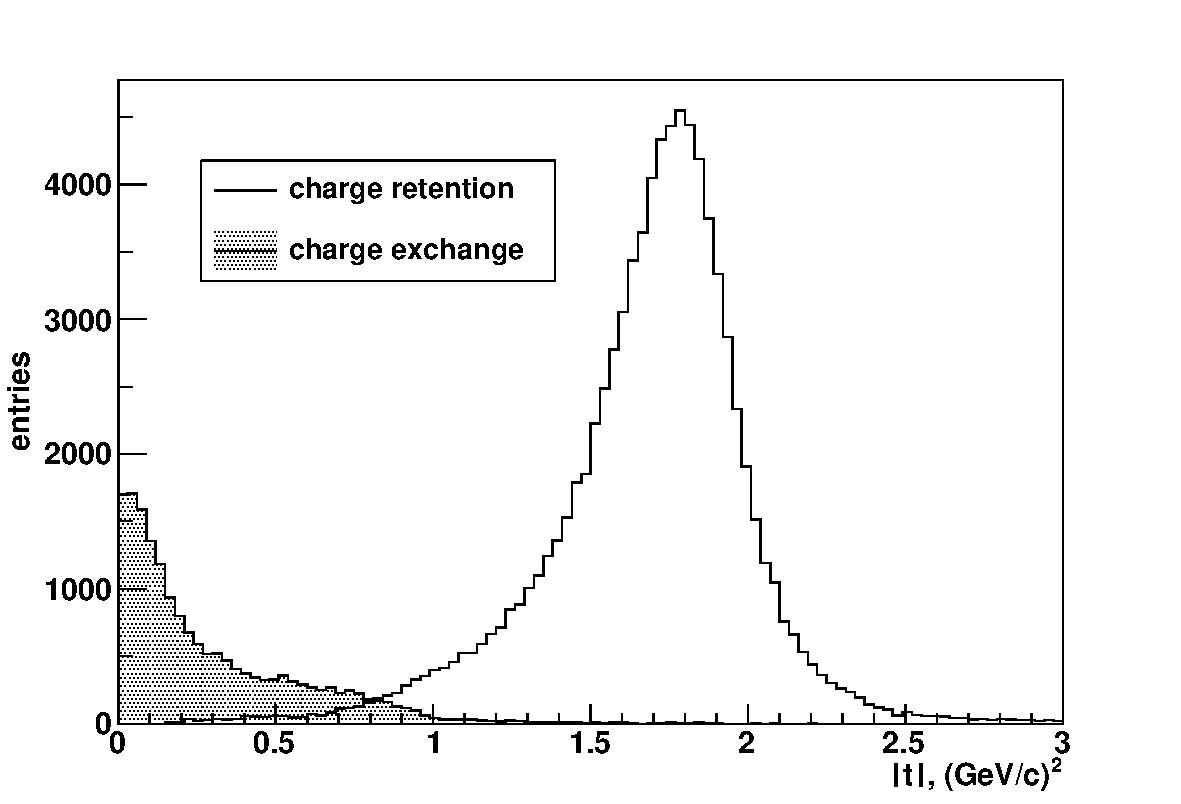
\includegraphics[width=1.00\textwidth]{chex_ret_t.pdf}
  \caption{Распределения событий реакции \dpfrag по квадрату четырёхмерного
    переданного импульса $|t|$ от протона-мишени к нейтрону. Заштрихованное
    распределение (charge exchange)~--- канал реакции перезарядки \dpchex,
    незаштрихованное (charge retention)~--- прямой канал реакции развала
    дейтрона \dpret.}
  \label{fig:chex_ret_t}
\end{figure}

В случае реакции перезарядки на дейтроне, благодаря применяемой методике
исследования (пучок ускоренных дейтронов), в конечном состоянии в лабораторной
системе координат наблюдается характерная топология событий~--- два выходящих
из точки взаимодействия быстрых протона с близкими импульсами и малым углом
раствора. Это способствует надёжному разделению на стереофотографиях реакции
перезарядки \dpchex с реакцией прямого канала развала дейтрона \dpret, в которой
один из двух протонов всегда медленный, что позволяет исследовать реакцию
перезарядки практически без потерь~\cite{balga88}.

Экспериментальные данные о реакции \dpfrag свидетельствуют о том, что этот
процесс, в основном, идёт с участием одного нуклона из дейтрона, тогда как
другой нуклон является спектатором. Спектатор~--- самый медленный из нуклонов в
системе покоя дейтрона (антилабораторная система), не принимавший участие во
взаимодействии (квази-упругое рассеяние). Рассеянным нуклоном называем,
наоборот, самый быстрый из нуклонов в системе покоя дейтрона. Оставшийся
фрагмент~--- нуклон отдачи. На рис.~\ref{fig:spec_reco_scat} приведены
импульсные распределения всех продуктов из реакции безмезонного развала дейтрона
\dpfrag в системе покоя дейтрона.

\begin{figure}[h]
  \centering
  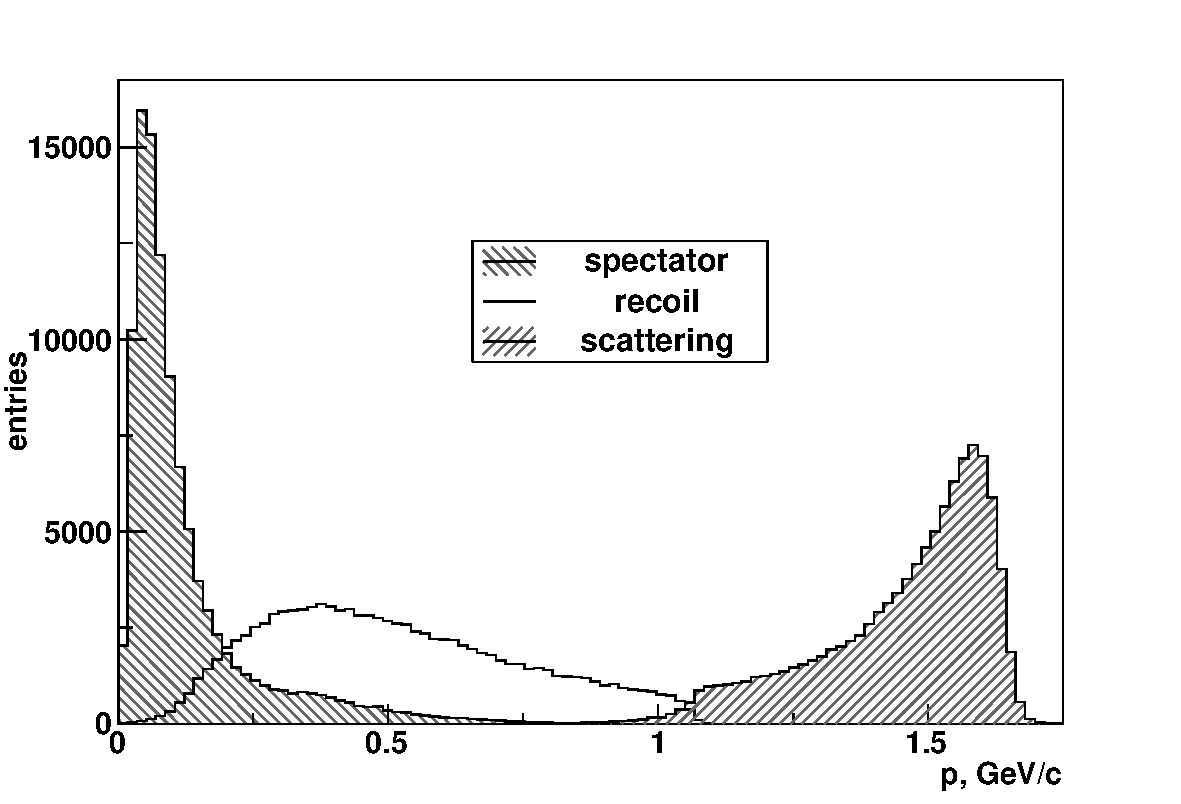
\includegraphics[width=1.00\textwidth]{spec_reco_scat.pdf}
  \caption{Импульсные распределения спектаторов (spectator), нуклонов отдачи
    (recoil) и рассеивающихся нуклонов (scattering) из реакции развала дейтрона
    \dpfrag в системе покоя дейтрона.}
  \label{fig:spec_reco_scat}
\end{figure}

В системе покоя дейтрона и в лабораторной системе координат определения нуклона
отдачи и рассеянного нуклона взаимно изменяются, а именно, нуклон отдачи в
системе покоя дейтрона, тот же, что и рассеянный нуклон в лабораторной системе
координат. В дальнейшем мы будем, как правило, использовать эти обозначения для
системы покоя дейтрона.

Так как при развале быстрого дейтрона \dpfrag в лабораторной системе спектаторы
имеют достаточно большие импульсы и их можно надёжно идентифицировать, потери
обусловлены, главным образом, событиями с малыми передачами импульса
протону-мишени (протону-отдачи). Однако, такие потери меньше, чем при упругом
рассеянии \dpela, так как при развале налетающего дейтрона наблюдается резкое
(примерно в два раза) изменение импульса, а следовательно, и кривизны трека в
магнитном поле у заряженных фрагментов по сравнению с падающим ядром. Кроме
того, для развала дейтрона необходимо затратить энергию порядка 2.2~МэВ (энергия
связи дейтрона), что приводит к отсутствию частиц отдач с малыми импульсами.

\begin{figure}[h]
  \centering
  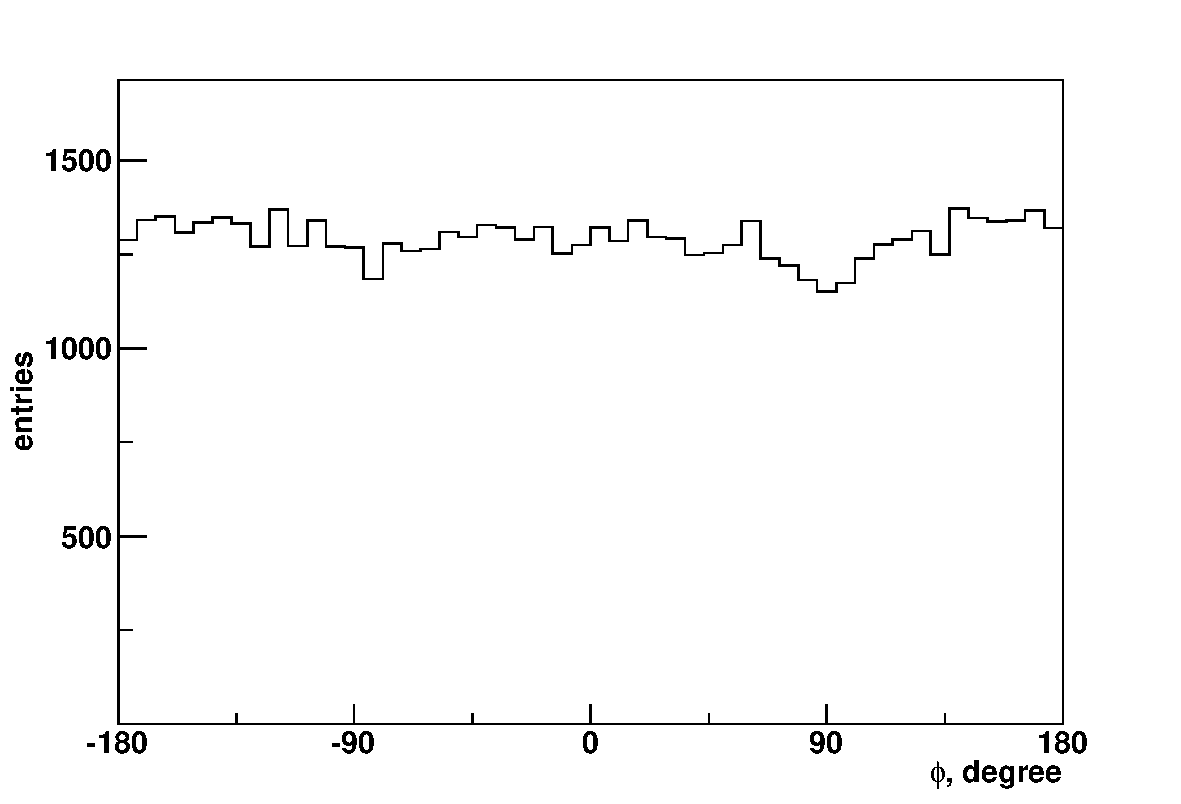
\includegraphics[width=1.00\textwidth]{phi_recoil.pdf}
  \caption{Распределение по азимутальному углу $\phi$ протонов отдачи в реакции
    развала ядра дейтрона \dpfrag.}
  \label{fig:phi_recoil}
\end{figure}

Поскольку надёжное наблюдение треков протонов в водородной камере начинается с
импульса выше приблизительно 80~МэВ/c (что соответствует длине трека в
пузырьковой камере порядка 1~мм)~\cite{niora91}, то потери в отборе событий с
развалом ядра дейтрона можно считать несущественными. Об этом можно судить из
распределения по азимутальному углу протонов отдачи в изучаемом нами канале
развала ядра дейтрона \dpfrag, и также, из распределения по поперечным импульсам
рассеивающихся нуклонов~\cite{alad75_3}. На рис.~\ref{fig:phi_recoil} показано
азимутальное распределение протонов отдачи в реакции развала дейтрона. Видно,
что оно практически изотропно во всём интервале азимутальных углов, т.е. потери
в реакции полного развала ядра дейтрона минимальные, несущественные.

\subsection{Сечение и миллибарн-эквивалент события}
Экспериментальный материал по дейтрон-протонным столкновениям содержит два
набора данных. Первый из них~--- $dp$-взаимодействия, полученные с
неполяризованным пучком в начале 70-х годов, и второй~--- данные, накопленные в
конце 80-х годов в пучке поляризованных дейтронов. Анализ и сравнение некоторых
основных характеристик взаимодействий поляризованных и неполяризованных
дейтронов с протонами показал их идентичность, что позволило объединить оба
набора экспериментальных данных~\cite{balga88}. В работе используются суммарные
данные из обеих наборов.

Для определения миллибарн-эквивалента события, из известного полного сечения
$dp$-реакции, необходимо было оценить экспериментальные потери событий в
$dp$-взаимодействиях. Как уже отмечалось, потери в отборе событий с развалом
ядра дейтрона можно считать несущественными. Основным видом потерь при поиске
событий были потери при малых переданных импульсах в упругих взаимодействиях
\dpela. Это хорошо видно из рис.~\ref{fig:phi_elastic}, где приводятся
распределения по азимутальному углу протонов отдачи в упругом $dp$-канале для
разных интервалов значения $|t|$. Распределения нормированы на максимум, чтобы
лучше показать их различие. Как видно, при малых передачах
$|t| < 0.06$~(ГэВ/с)$^2$ (заштрихованное распределение) наблюдается отклонение
от изотропии, обусловленное потерями в этой области переданного четырёхимпульса.
При более высоких передачах $|t| > 0.06$~(ГэВ/с)$^2$ распределение
(незаштрихованное) становится изотропным.

\vspace{-0.1cm}
\begin{figure}[h]
  \centering
  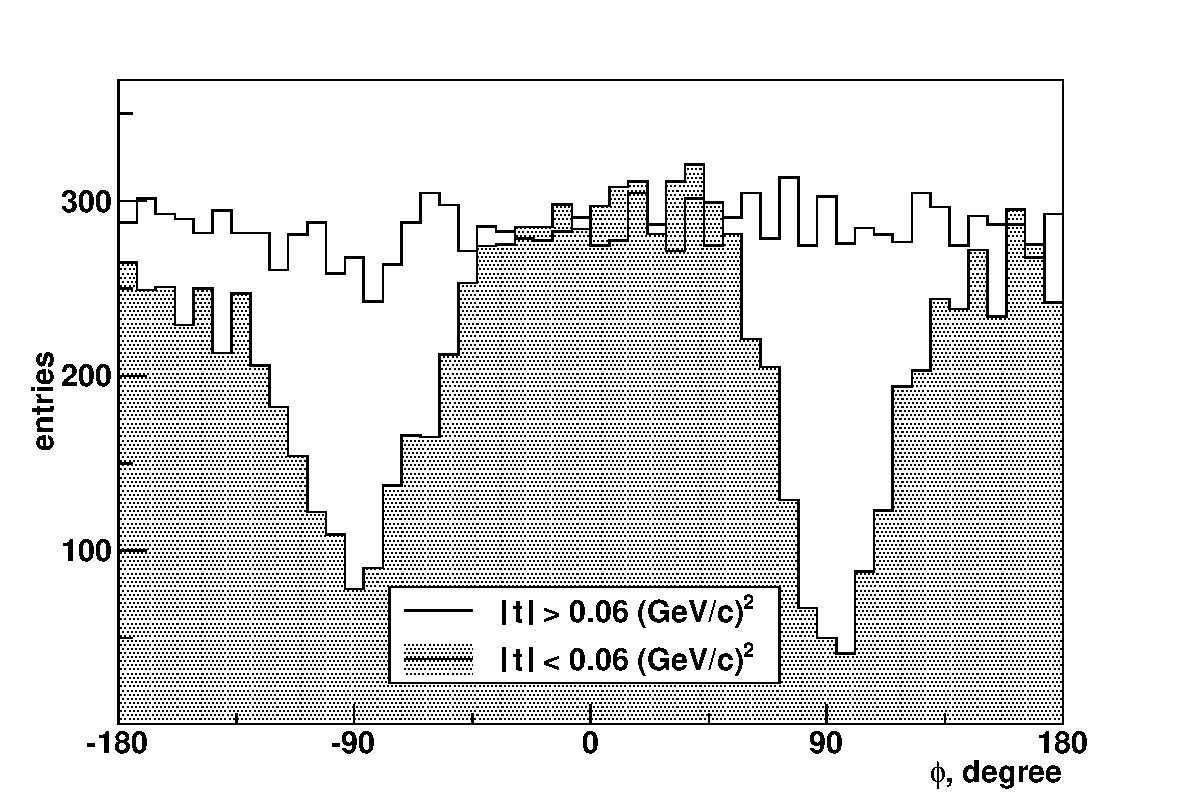
\includegraphics[width=1.00\textwidth]{phi_elastic.pdf}
  \caption{Распределения по азимутальному углу $\phi$ протонов отдачи в реакции
    упругого рассеяния \dpela (нормированы на максимум). Заштрихованное
    распределение при значениях $|t| < 0.06$ (ГэВ/с)$^2$, незаштрихованное при
    $|t| > 0.06$ (ГэВ/с)$^2$.}
  \label{fig:phi_elastic}
\end{figure}

Реально принималось, что случайные потери по каналам реакции $dp \rightarrow X$
пропорциональны вкладам каналов, а систематические потери сосредоточены только в
упругом канале \dpela и связаны с рассеянием на малые углы. Эти потери прямо
отражались на поведении дифференциального сечения упругого $dp$-рассеяния и
оценивались по экспериментальным данным.

\begin{figure}[h]
  \centering
  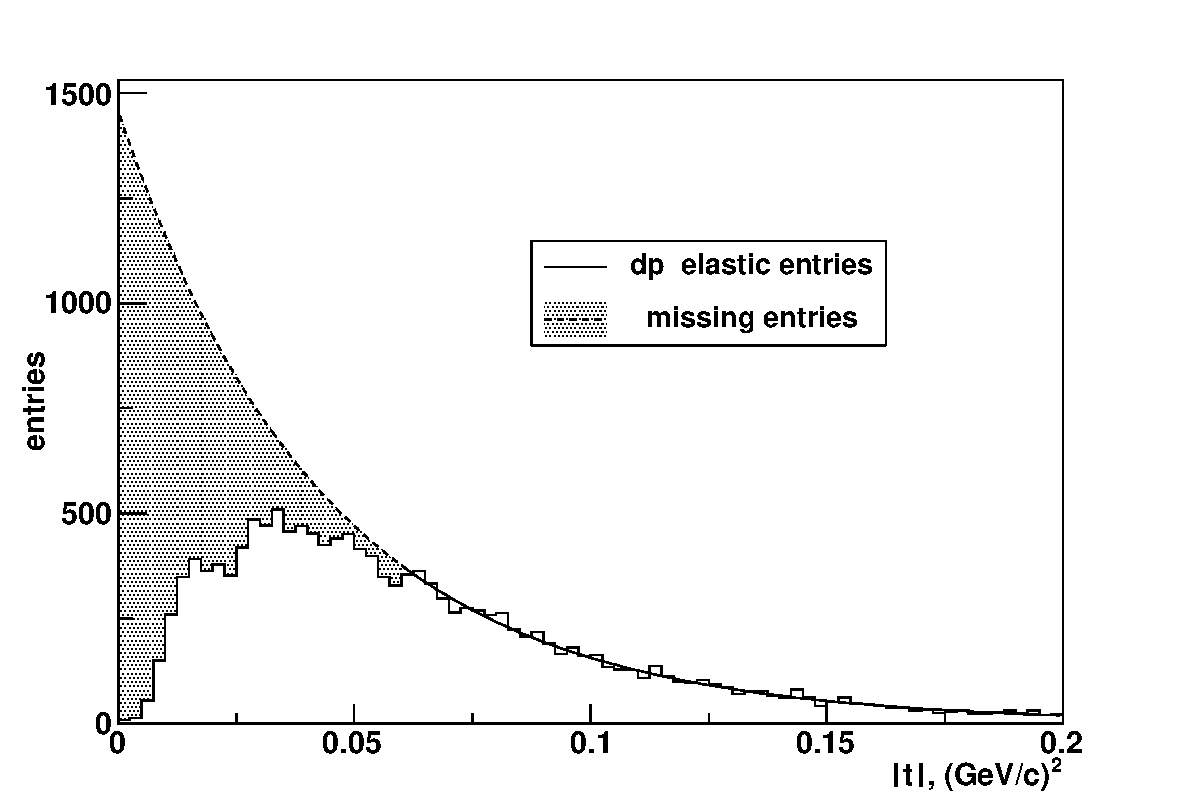
\includegraphics[width=1.00\textwidth]{dp_dp_t.pdf}
  \caption{Распределение событий упругого рассеяния \dpela по квадрату
    четырёхмерного переданного импульса $|t|$. Заштрихованная область (missing
    entries) представляет события потерянные в этом канале. Штриховая линия~---
    экстраполяция аппроксимирующей функцией в область потерь
    $|t| < 0.06$~(ГэВ/с)$^2$.}
  \label{fig:dp_dp_t}
\end{figure}

Число потерянных событий при малых передачах $|t|$ в реакции упругого
$dp$-рассеяния оценивалось путём аппроксимации распределения на
рис.~\ref{fig:dp_dp_t} двойной экспоненциальной функцией и затем экстраполяцией
в область $|t| < 0.06$ (ГэВ/с)$^2$. Процедура аппроксимации этой функцией была
применена только для той области четырёхимпульса $|t|$, где потеря событий
практически отсутствовала, т.е. $0.06 < |t| < 0.20$ (ГэВ/с)$^2$. В результате
было найдено, что систематические потери в реакции упругого рассеяния \dpela
составляют приблизительно 10500 событий.

Значение миллибарн-эквивалента события определялось исходя из полного сечения
$dp$-взаимодействий~\cite{bugg66} (82.89~$\pm$~0.06)~мб при импульсе 3.35~ГэВ/с,
с учётом потерь событий упругого $dp$-рассеяния, и равно
(0.0003342~$\pm$~0.0000007)~мб/событие (ошибка статистическая). Систематическая
ошибка, связанная с оценкой потерь событий в упругом $dp$-рассеянии, составляла
около 4~$\%$.

Проведённое нами определение вклада спин-зависящей части амплитуды элементарного
\np рассеяния (следующий раздел) основано на анализе событий выделенной реакции
перезарядки \dpchex. Число событий реакции перезарядки равно 17512, что
соответствует поперечному сечению (5.85~$\pm$~0.05)~мб. Заметим, что это сечение
включает в себя часть событий квази-$pp$ рассеяния с образованием промежуточной
$\Delta$-изобары.

\section{Реакция перезарядки \maybebm{{\dpchex}}}
В предыдущей главе диссертации были обсуждены идеи, впервые высказанные в
работах Померанчука и Чу, указавшие на возможность использования
зарядово-обменных процессов на дейтроне для извлечения дополнительной информации
по амплитуде элементарной \np реакции. По мере увеличения статистики событий на
водородной камере нами была сделана экспериментальная оценка вклада
спин-зависящей части амплитуды элементарного \np процесса.

Математический формализм, используемый для определения вклада спин-зависящей
части амплитуды $np$-рассеяния в процессе перезарядки на дейтроне, развитый в
работах Дина и др. более подробно рассматривался в первой главе,
раздел~\ref{section:theory}. Напомним некоторые из теоретических формул.
Дифференциальное поперечное сечение \np рассеяния может быть представлено в виде
суммы спин-независящей и спин-зависящей частей
\begin{equation}
  \label{eq:np}
  (d\sigma/dt)_{\np} = (d\sigma/dt)^{SI}_{\np} + (d\sigma/dt)^{SD}_{\np}\,.
\end{equation}
В рамках импульсного приближения можно записать соотношение между
дифференциальным поперечным сечением реакции перезарядки на дейтроне \dpchex и
процессом элементарной перезарядки \np в следующем виде
\begin{equation}
  \label{eq:dpnp}
  (d\sigma/dt)_{\dpchex} = [1-F_d(t)]\,(d\sigma/dt)^{SI}_{\np} +
        [1-1/3\,F_d(t)]\,(d\sigma/dt)^{SD}_{\np}\,.
\end{equation}

При нулевом переданном импульсе ($t=0$) от протона-мишени к нейтрону, т.е. при
угле рассеяния 180$^{\,\circ}$ в системе центра масс, из-за того, что формфактор
дейтрона $F_d(0) = 1$, дифференциальное поперечное сечение перезарядки на
дейтроне будет равно
\begin{equation}
  \label{eq:dpnp0}
  (d\sigma/dt)_{\dpchex} = 2/3\,(d\sigma/dt)^{SD}_{\np}\,.
\end{equation}

Таким образом, реакция перезарядки неполяризованного дейтрона на
неполяризованном протоне-мишени при нулевой передаче импульса полностью
определяется спин-зависящей частью элементарного $np$-рассеяния назад. Анализ
процесса \dpchex при малых переданных импульсах, близких к нулю, позволяет
оценить вклад спин-зависящей части амплитуды реакции перезарядки \np. В
изучаемом канале реакции перезарядки это подтвердилось наличием ненулевого
дифференциального поперечного сечения $(d\sigma/dt)$ при малых, близких к нулю,
значениях $t$~(рис.~\ref{fig:chex_ret_t}~и~\ref{fig:dp_two_protons}).

Формулы выведены в определённых предположениях. Чтобы воспользоваться этими
выражениями, мы должны выполнить по крайней мере два условия, а именно
\begin{itemize}
\item работать в области малых переданных импульсов квази-упругого
  $np$-рассеяния и
\item принять справедливость импульсного приближения.
\end{itemize}
Было показано~\cite{glagolev99,led04}, что при релятивистских энергиях
применимость импульсного приближения оправдана. В работах по изучению
безмезонного развала дейтрона протонами в эксклюзивной постановке при импульсе
дейтрона 3.3~ГэВ/с подтвердилась справедливость импульсного
приближения~\cite{alad75_4,alad77_2,glagolev73}. Критерием выделения
области импульсного приближения служили изотропия в распределении угла
Треймана"--~Янга~\cite{trei62} и форма импульсного распределения нуклонов
спектаторов.

Условие импульсного приближения предполагает отсутствие взаимодействия в
конечном состоянии (ВКС). При экспериментальном исследовании механизма ВКС
наблюдалось, что этот эффект сильно проявляется в асимметрии распределений по
углу Треймана"--~Янга. Более естественной переменной, чем угол Треймана"--~Янга,
оказался угол Вилкина $\alpha$, который был введён при теоретических расчётах
ВКС для безмезонного развала дейтрона. В работе~\cite{alad77} было предложено
рассмотреть распределение событий в зависимости от угла $\alpha$ между импульсом
спектатора $\vec{p_s}$ и трёхмерным переданным импульсом $\vec{q}$ от
налетающего нуклона к рассеянному
\begin{equation}
  \cos{\alpha} = \frac{(\vec{p_s}\cdot\vec{q})}
      {|\,\vec{p_s}\,|\,|\,\vec{q}\,|}\,.
\end{equation}

Напомним, что спектатором называем нуклон, который является самым медленным из
вторичных нуклонов в системе покоя дейтрона, а рассеянным, самый быстрый из
них. В случае реакции перезарядки \dpchex рассеянным нуклоном становится
нейтрон, а спектатор и нуклон отдачи~--- протоны.

Информацию об угловых распределениях в зависимости от импульса спектатора можно
систематизировать с помощью параметра асимметрии $A$, определённого следующим
образом
\begin{equation}
  A = \frac{N(\alpha < 90^{\,\circ}) - N(\alpha > 90^{\,\circ})}
  {N(\alpha < 90^{\,\circ}) + N(\alpha > 90^{\,\circ})}\,,
\end{equation}
где $N$~--- число событий в указанных интервалах (полусферах) по углу
$\alpha$. Асимметрия представляет собой относительную разность числа событий в
передней и задней $\alpha$-полусфере.

На рис.~\ref{fig:asymmetry_alpha} показаны зависимости асимметрии по углу
$\alpha$ от импульса спектатора, как для реакции прямого канала, так и для
реакции перезарядки. Вследствие ограниченной статистики камерного эксперимента
полученные данные были разделены на две области по передаче четырёхмерного
импульса, $|t| < 0.1$ ГэВ/с$^2$ и область $0.1 < |t| < 0.3$ ГэВ/с$^2$. Как видно
из рисунка, наблюдается сильная зависимость асимметрии по углу $\alpha$ от
импульса спектатора, особенно для событий в области с меньшими $|t|$. Форма
экспериментальных распределений для двух областей $|t|$ похожа, но для больших
$|t|$, место, где асимметрия становится ненулевой, сдвинуто к более высоким
значениям импульса, что в согласии с теорией~\cite{alad77}. В случае реакции
развала дейтрона с перезарядкой (пустые кружки) зависимость асимметрии по углу
$\alpha$ менее выразительна, чем в канале прямого развала (сплошные кружки).

\begin{figure}[hp]
  \centering
  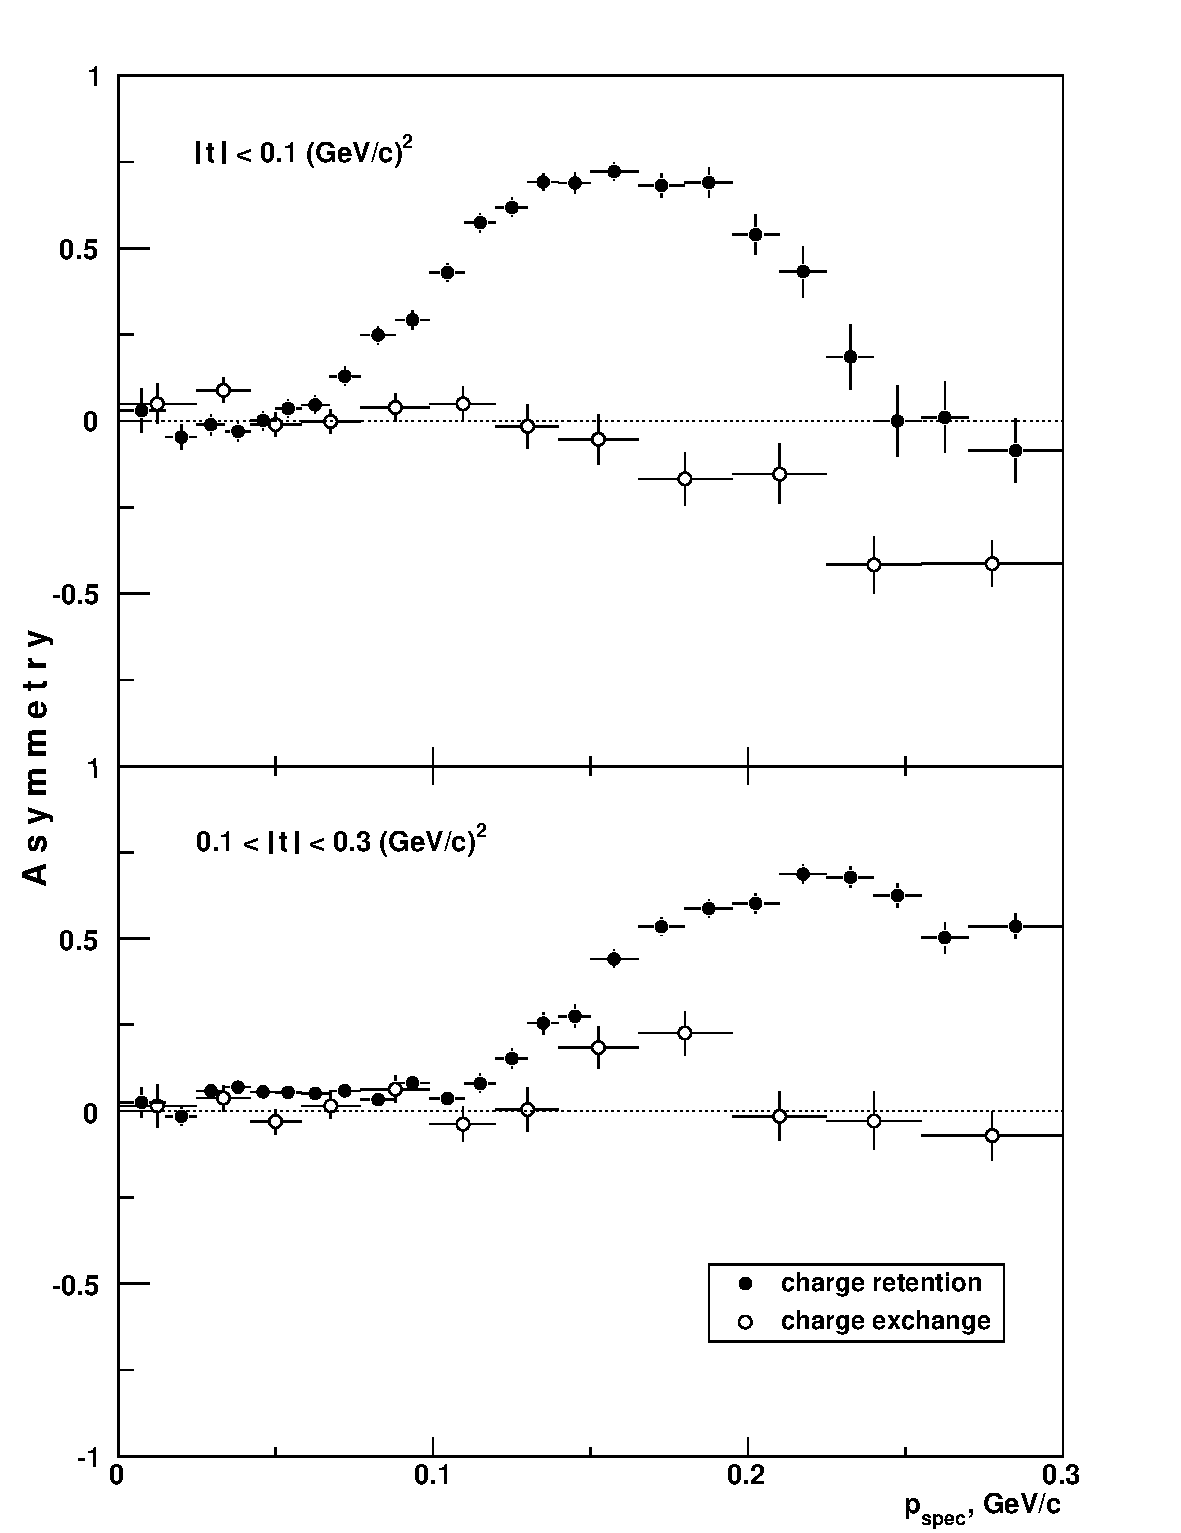
\includegraphics[width=1.00\textwidth]{asymmetry_alpha.pdf}
  \caption{Зависимость асимметрии по углу $\alpha$ от импульса спектатора
    $p_{spec}$ в системе покоя дейтрона для двух разных областей переданного
    четырёхимпульса $|t|$. Сплошные кружки~--- реакция прямого развала дейтрона
    \dpret, пустыми кружками обозначена реакция перезарядки \dpchex.}
  \label{fig:asymmetry_alpha}
\end{figure}

Таким образом, наблюдаемая сильная импульсная зависимость параметра асимметрии
по углу $\alpha$ в реакции прямого развала дейтрона вызвана взаимодействием в
конечном состоянии между протоном и нейтроном. Такое поведение может приводить
к объединению (слипанию) протона и нейтрона в конечном состоянии в дейтрон с
переходом части событий из реакции прямого развала \dpret в конкурирующий канал
реакции упругого рассеяния \dpela.

Однако, в области малых переданных импульсов $|t| < 0.1$ ГэВ/с$^2$ и импульсов
спектаторов меньших приблизительно 0.1~ГэВ/с, асимметрии по углу $\alpha$,
вызванные ВКС, практически отсутствуют (близки к нулю). Это хорошо видно
(рис.~\ref{fig:asymmetry_alpha}), как для прямого развала дейтрона, так и для
развала дейтрона с перезарядкой, где асимметрия менее выразительна и становится
отличной от нуля при заметно больших значениях импульса спектатора. Такое
поведение асимметрии по углу $\alpha$ также указывает на возможность применения
импульсного приближения в интересующей нас области малых переданных импульсов и
малых импульсов спектаторов.

Кроме вышесказанного, условие импульсного приближения означает необходимость
работать в области малых импульсов нуклонов в дейтроне, т.е. в области
преобладания $S$-волны в волновой функции дейтрона. Это видно, например из
рис.~\ref{fig:S_waves}, на котором показана вероятность $S$-волны в зависимости
от импульса внутреннего движения нуклонов в дейтроне. Согласно расчётам с
различными реалистическими потенциалами, в области до $p \simeq 0.07$~ГэВ/с
эта вероятность практически не зависит от импульса внутреннего движения нуклонов
в дейтроне и близка к единице (вне области влияния $D$-волны).

\begin{figure}[h]
  \centering
  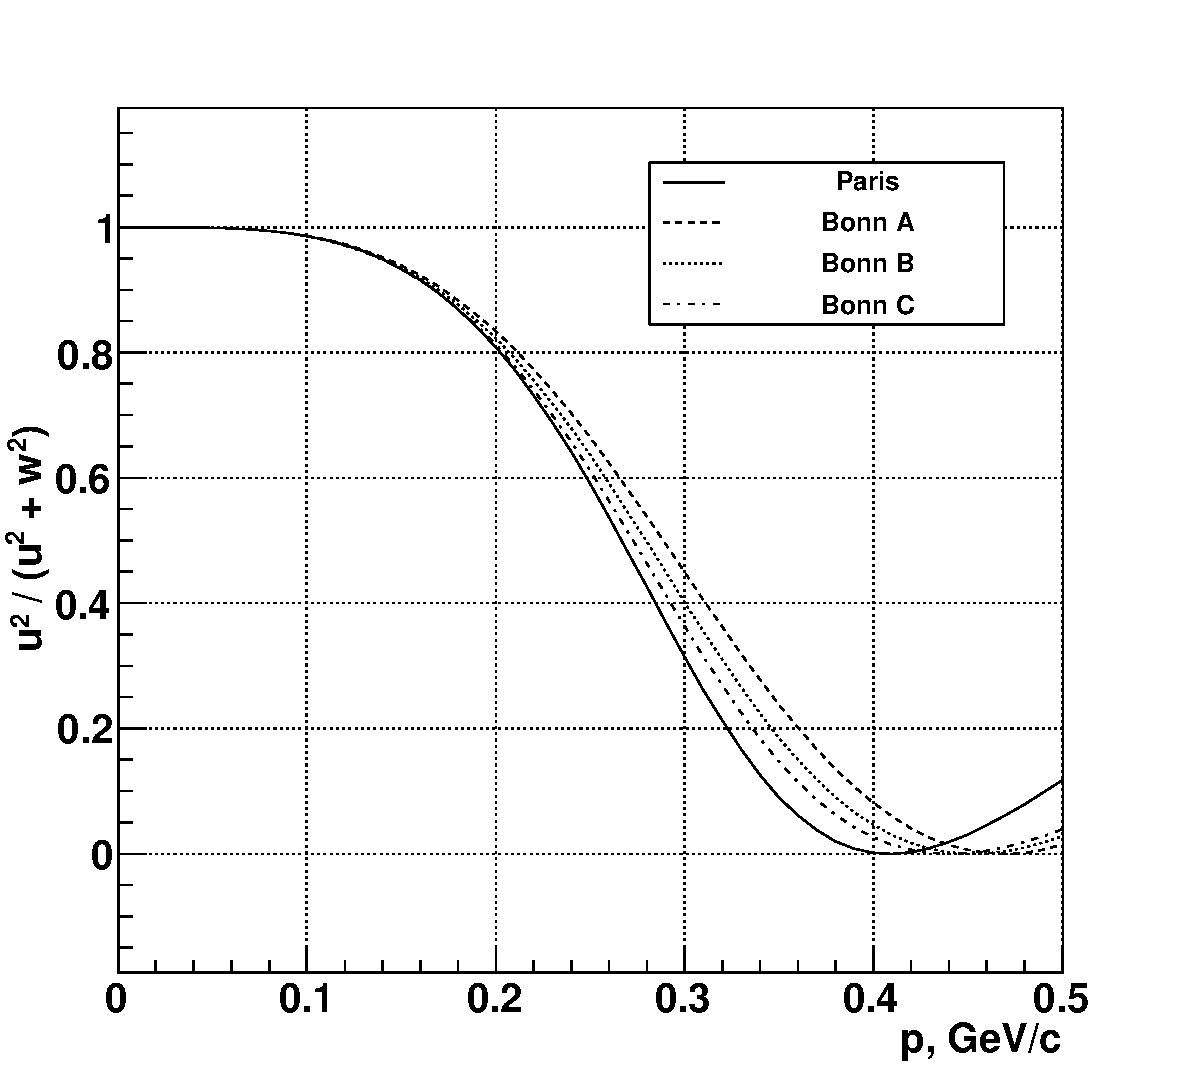
\includegraphics[width=0.79\textwidth]{S_waves.pdf}
  \caption{Вероятность $S$-волны в волновой функции дейтрона в зависимости от
    Ферми импульса $p$ нуклонов в дейтроне. $u$ и $w$~--- соответственно $S$ и
    $D$ волновые функции рассчитанные с различными реалистическими
    потенциалами.}
  \label{fig:S_waves}
\end{figure}

Предположения, при которых были выведены формулы~\eqref{eq:dpnp} и
\eqref{eq:dpnp0}, можно одновременно удовлетворить, отбирая на эксперименте
такие события, в которых в лабораторной системе координат (быстрый дейтрон
падает на покоящуюся протонную мишень) два быстрых протона из реакции
перезарядки \dpchex вылетают под малыми углами по отношению к падающему дейтрону
и с импульсами близкими к половине импульса дейтрона. Подчеркнём здесь, что
поставленная задача может быть экспериментально выполнена только при наличии
ускоренных дейтронов. В случае падающего быстрого протона на покоящуюся
дейтронную мишень, вторичные протоны из такой реакции перезарядки
$pd \rightarrow n(pp)$ будут слишком медленными, чтобы их зарегистрировать, а
сама реакция не может быть идентифицирована.

\begin{figure}[hp]
  \centering
  % 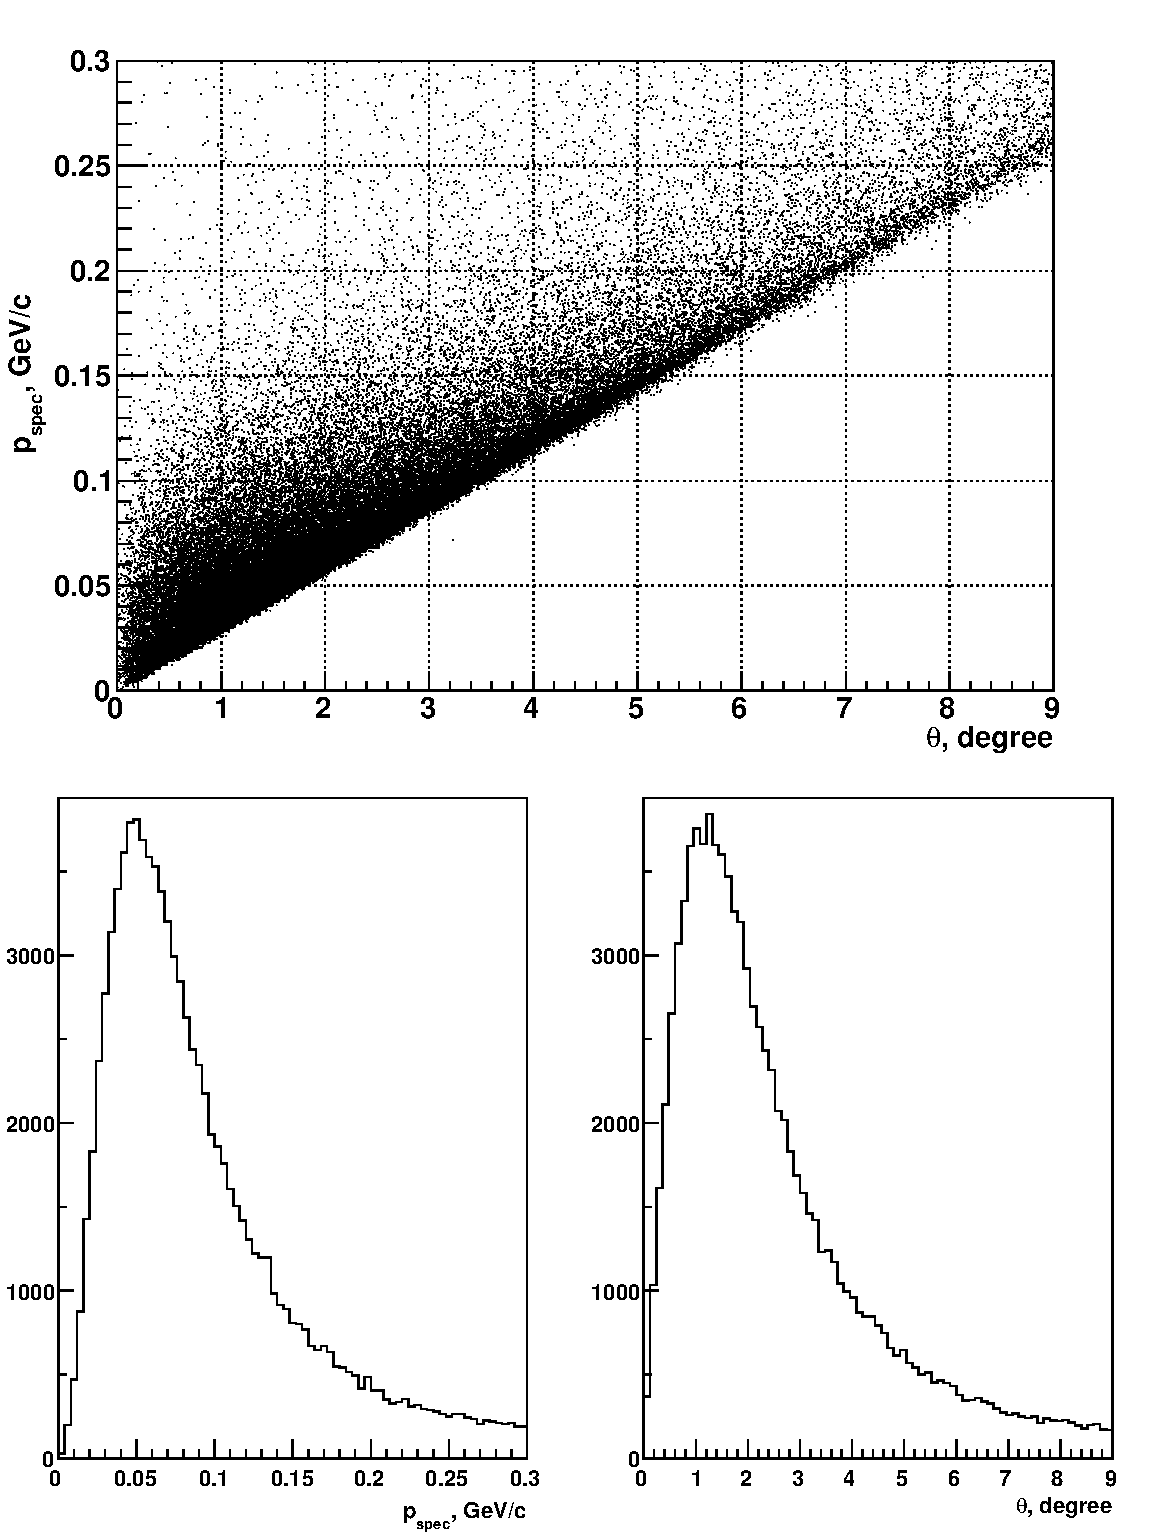
\includegraphics[width=1.00\textwidth]{theta_p.pdf}
  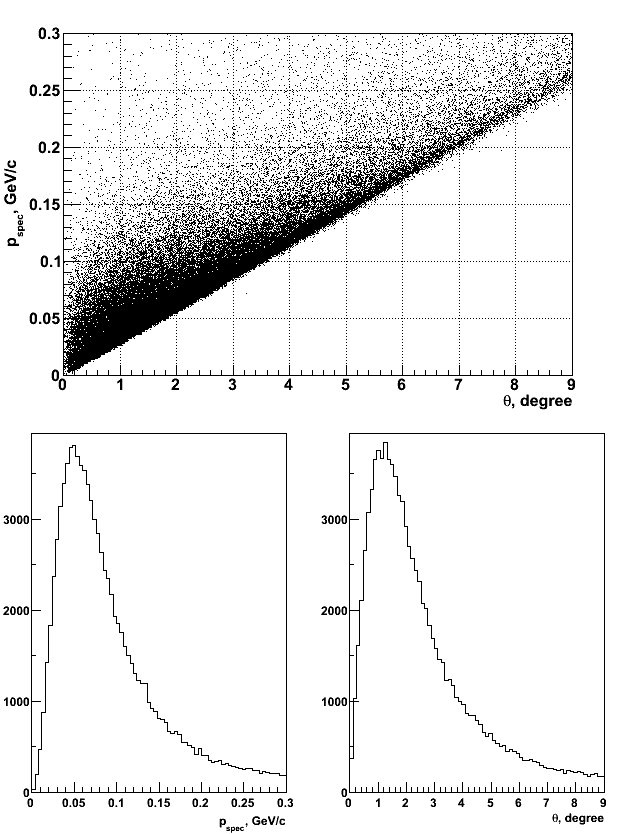
\includegraphics[width=1.00\textwidth]{theta_p.png}
  \caption{Зависимость полярного угла вылета $\theta$ спектатора в лабораторной
    системе координат от его импульса $p_{spec}$ в системе покоя дейтрона из
    реакции развала дейтрона на протоне. Под двумерным распределением показаны
    проекции на оси координат.}
  \label{fig:theta_p}
\end{figure}

Воспользуемся кинематической корреляцией между полярным углом вылета нуклона
спектатора в лабораторной системе координат и его импульсом в системе покоя
дейтрона приведённой на рис.~\ref{fig:theta_p}. Видно, что при углах меньших
порядка 5$^{\,\circ}$, или при импульсе спектатора меньше $\sim$~0.15 ГэВ/с,
лежит основная часть событий, соответствующих квази-нуклонному рассеянию. В
случае, когда передача четырёхмерного импульса (от протона-мишени к нейтрону)
стремится к нулю $|t| \rightarrow 0$, два быстрых протона из реакции перезарядки
в лабораторной системе координат имеют практически одинаковые импульсы близкие к
половине импульса дейтрона $p_{p_1} \simeq p_{p_2} \simeq (1/2)\,p_d$.

\begin{figure}[h]
  \centering
  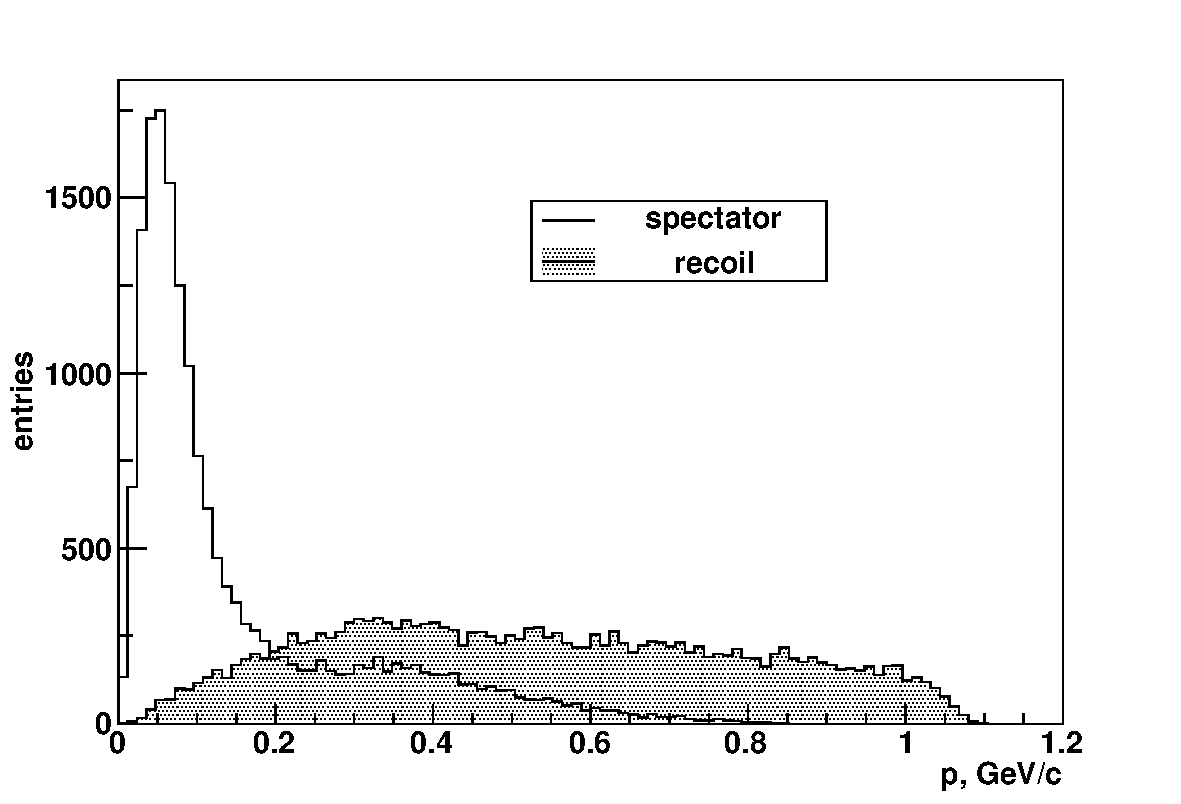
\includegraphics[width=1.00\textwidth]{spec_reco_p.pdf}
  \caption{Импульсные распределения протонов спектаторов (незаштрихованное) и
    протонов отдачи (заштрихованное) в система покоя дейтрона из реакции
    перезарядки дейтрона на протоне \dpchex.}
  \label{fig:spec_reco_p}
\end{figure}

\begin{figure}[hp]
  \centering
  \vspace{-0.2cm}
  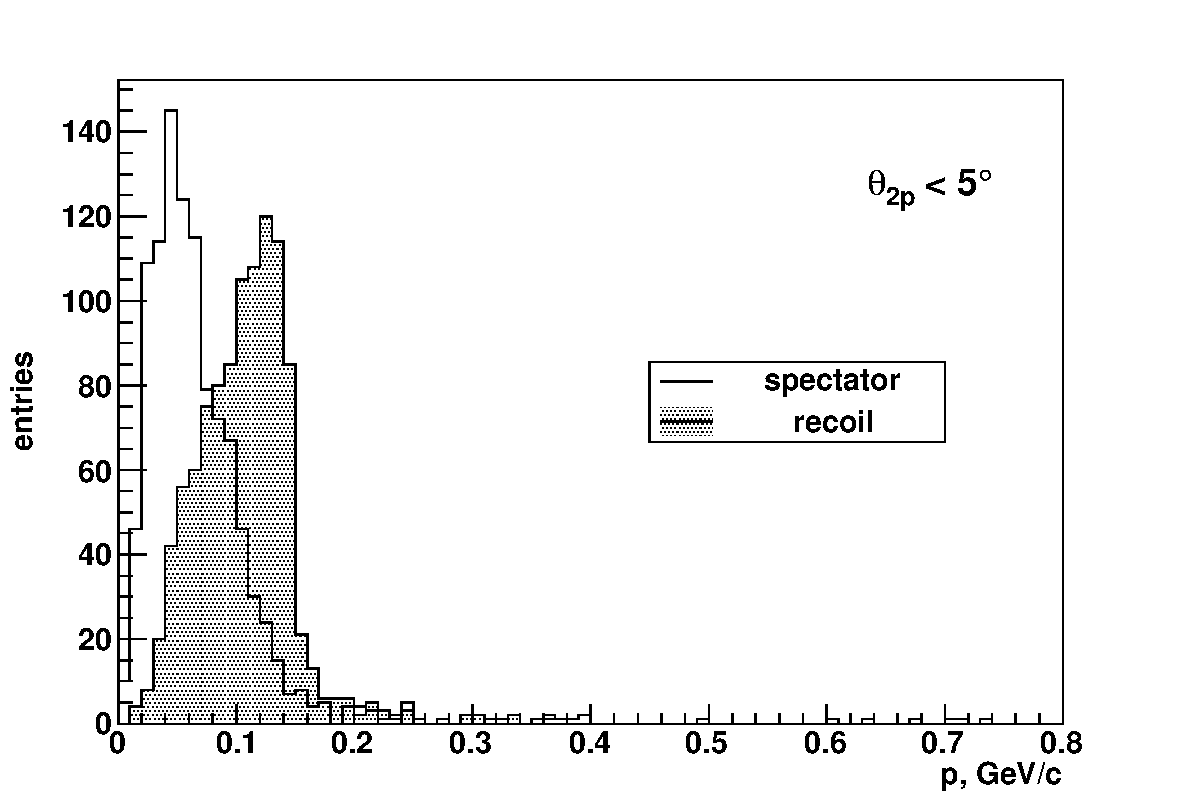
\includegraphics[width=0.99\textwidth]{spec_reco_p_5.pdf}
  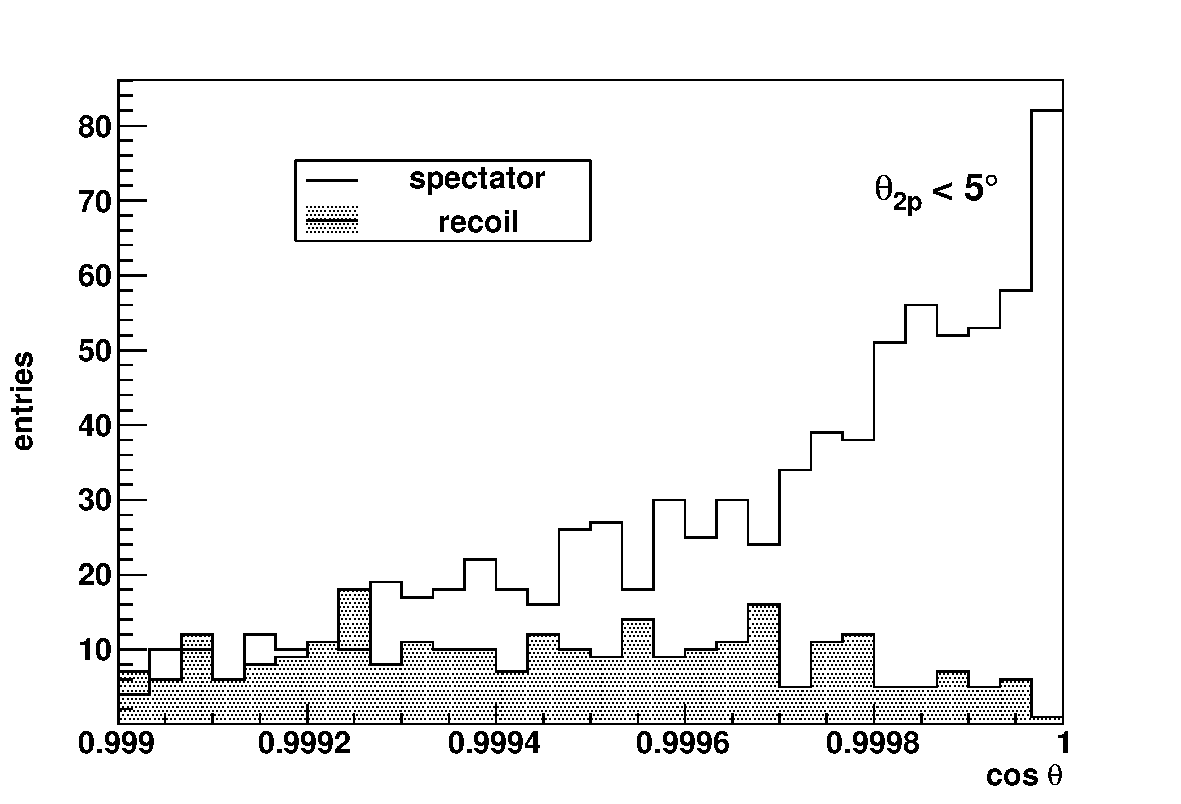
\includegraphics[width=0.99\textwidth]{spec_reco_cost_5.pdf}
  \caption{На верхнем рисунке те же самые распределения как на
    рис.~\ref{fig:spec_reco_p}, но при ограничении угла раствора конуса
    для обоих протонов в лабораторной системе координат меньше 5$^{\,\circ}$.
    Нижний рисунок~--- угловые распределения таких протонов в лабораторной
    системе координат.}
  \label{fig:spec_reco_5}
\end{figure}

Импульсные распределения двух протонов (протонов спектаторов и протонов отдачи)
из реакции перезарядки \dpchex показаны на рис.~\ref{fig:spec_reco_p}. Как
видно, если не вводить никаких ограничений на их углы вылета, импульсные
распределения этих двух протонов существенно различаются. Вид распределения
импульсов протонов спектаторов (незаштрихованное) является характерным для Ферми
движения нуклонов в дейтроне. При ограничении угла раствора конуса, в пределах
которого вылетают оба протона, в лабораторной системе координат примерно
в~5$^{\,\circ}$, распределения спектаторов и протонов отдачи значительно
перекрываются, рис.~\ref{fig:spec_reco_5}. На том же рисунке (внизу) показаны и
их угловые распределения. В итоге, отбирая события, когда пара протонов попадает
в конус с раствором меньше 5$^{\,\circ}$, будет построено распределение
дифференциального поперечного сечения реакции перезарядки дейтрона на протоне
$(d\sigma/dt)_{\dpchex}$ при малых переданных импульсах.

\subsection{События с участием промежуточной
  $\maybebm{\Delta}$-изобары.}
Прежде чем перейти к извлечению информации о вкладе спин-зависящей части
амплитуды элементарного $np$-рассеяния, необходимо оценить вклад событий с
образованием промежуточной $\Delta$-изобары. В
работах~\cite{alad75_2,alad76,alad79}
по изучению реакции безмезонного развала дейтрона на протонах было впервые
показано, что высокоимпульсная часть спектра нуклонов спектаторов в реакции
перезарядки заметно больше, чем в прямом канале. Такой эффект объяснялся вкладом
неупругих процессов с обменом промежуточной $\Delta$-изобарой, основная часть
которых является следствием квази-$pp$ столкновений, идущих через рождение
$\Delta^{++}$-изобары, диаграмма б) Фейнмана из рис.~\ref{fig:feynman}. Это
связано с большим сечением образования промежуточной $\Delta^{++}$-изобары
(канал развала дейтрона с зарядовым обменом) относительно остальных $\Delta^{+}$
и $\Delta^{\circ}$-состояний~\cite{dol86}.
% mf '\mode:=localfont; input ppn_fmf'
% mpost '\mode:=localfont; input ppn_fmf'
\begin{figure}[!h]
  \begin{center}
    \begin{fmffile}{ppn_fmf}
      \vspace{15mm}
      \hspace{-10mm}
      % pp1, delta+
      \parbox{0.45\textwidth} {
        \begin{fmfgraph*}(70,35)
          \fmfset{arrow_len}{5mm}\fmfset{arrow_ang}{10}
          \fmfleft{iA,iB}
          \fmfright{o1,o2,o3}
          \fmflabel{$d$}{iA}
          \fmflabel{$p$}{iB}
          \fmflabel{$p$}{o3}
          \fmflabel{$n$}{o2}
          \fmflabel{$p$}{o1}

          \fmf{fermion,tension=1.0}{iA,v1} % default tension=1.0
          \fmf{fermion,tension=1.0}{v2,o1}
          \fmf{fermion,tension=1.0}{v2,o2}
          \fmf{fermion,tension=1.0}{iB,v3,o3}

          \fmf{fermion,tension=1.5,label=$n$}{v1,v2}
          \fmf{fermion,tension=0.2,lab.side=left,label=$p$}{v1,v3}
          \fmf{fermion,tension=0.1,lab.side=left,label=$\Delta^{+}$}{v3,v2}

          \fmfblob{0.06w}{v1}
          \fmfdot{v2,v3}
          \fmf{dbl_plain_arrow}{iA,v1}
          \fmffreeze
          \fmf{plain_arrow,width=2.5*thin}{v3,v2}
        \end{fmfgraph*}
      }
      % pp2, delta++
      \qquad
      \parbox{0.45\textwidth} {
        \begin{fmfgraph*}(70,35)
          \fmfset{arrow_len}{5mm}\fmfset{arrow_ang}{10}
          \fmfleft{iA,iB}
          \fmfright{o1,o2,o3}
          \fmflabel{$d$}{iA}
          \fmflabel{$p$}{iB}
          \fmflabel{$n$}{o3}
          \fmflabel{$p$}{o2}
          \fmflabel{$p$}{o1}

          \fmf{fermion,tension=1.0}{iA,v1} % default tension=1.0
          \fmf{fermion,tension=1.0}{v2,o1}
          \fmf{fermion,tension=1.0}{v2,o2}
          \fmf{fermion,tension=1.0}{iB,v3,o3}

          \fmf{fermion,tension=1.5,label=$n$}{v1,v2}
          \fmf{fermion,tension=0.2,lab.side=left,label=$p$}{v1,v3}
          \fmf{fermion,tension=0.1,lab.side=left,label=$\Delta^{++}$}{v3,v2}

          \fmfblob{0.06w}{v1}
          \fmfdot{v2,v3}
          \fmf{dbl_plain_arrow}{iA,v1}
          \fmffreeze
          \fmf{plain_arrow,width=2.5*thin}{v3,v2}
        \end{fmfgraph*}
      }
      \begin{center}
        \vspace{5mm}
        а) \hspace{75mm} б)
      \end{center}
      % np1, delta+
      \vspace{15mm}
      \hspace{-10mm}
      \parbox{0.45\textwidth} {
        \begin{fmfgraph*}(70,35)
          \fmfset{arrow_len}{5mm}\fmfset{arrow_ang}{10}
          \fmfleft{iA,iB}
          \fmfright{o1,o2,o3}
          \fmflabel{$d$}{iA}
          \fmflabel{$p$}{iB}
          \fmflabel{$n$}{o3}
          \fmflabel{$p$}{o2}
          \fmflabel{$p$}{o1}

          \fmf{fermion,tension=1.0}{iA,v1} % default tension=1.0
          \fmf{fermion,tension=1.0}{v2,o1}
          \fmf{fermion,tension=1.0}{v2,o2}
          \fmf{fermion,tension=1.0}{iB,v3,o3}

          \fmf{fermion,tension=1.5,label=$p$}{v1,v2}
          \fmf{fermion,tension=0.2,lab.side=left,label=$n$}{v1,v3}
          \fmf{fermion,tension=0.1,lab.side=left,label=$\Delta^{+}$}{v3,v2}

          \fmfblob{0.06w}{v1}
          \fmfdot{v2,v3}
          \fmf{dbl_plain_arrow}{iA,v1}
          \fmffreeze
          \fmf{plain_arrow,width=2.5*thin}{v3,v2}
        \end{fmfgraph*}
      }
      % np2, delta0
      \qquad
      \parbox{0.45\textwidth} {
        \begin{fmfgraph*}(70,35)
          \fmfset{arrow_len}{5mm}\fmfset{arrow_ang}{10}
          \fmfleft{iA,iB}
          \fmfright{o1,o2,o3}
          \fmflabel{$d$}{iA}
          \fmflabel{$p$}{iB}
          \fmflabel{$p$}{o3}
          \fmflabel{$n$}{o2}
          \fmflabel{$p$}{o1}

          \fmf{fermion,tension=1.0}{iA,v1} % default tension=1.0
          \fmf{fermion,tension=1.0}{v2,o1}
          \fmf{fermion,tension=1.0}{v2,o2}
          \fmf{fermion,tension=1.0}{iB,v3,o3}

          \fmf{fermion,tension=1.5,label=$p$}{v1,v2}
          \fmf{fermion,tension=0.2,lab.side=left,label=$n$}{v1,v3}
          \fmf{fermion,tension=0.1,lab.side=left,label=$\Delta^{\circ}$}{v3,v2}

          \fmfblob{0.06w}{v1}
          \fmfdot{v2,v3}
          \fmf{dbl_plain_arrow}{iA,v1}
          \fmffreeze
          \fmf{plain_arrow,width=2.5*thin}{v3,v2}
        \end{fmfgraph*}
      }
      \begin{center}
        \vspace{5mm}
        в) \hspace{75mm} г)
      \end{center}
    \end{fmffile}

    \caption{Диаграммы Фейнмана для реакции безмезонного развала дейтрона на
      протоне \dpfrag с образованием промежуточной $\Delta$-изобары. Диаграммы
      а) и б) соответствуют событиям с участием $\Delta^{+}$ и
      $\Delta^{++}$-изобары в квази-$pp$ столкновениях. События с обменом заряда
      изображены на диаграммах б) и в).}
    \label{fig:feynman}
  \end{center}
\end{figure}



%%% Local Variables:
%%% mode: latex
%%% TeX-master: "../musinsky_disser"
%%% coding: utf-8
%%% End:


Импульсные распределения нуклонов спектаторов (нормированные на максимум) из
реакции перезарядки на дейтроне \dpchex и реакции прямого канала с сохранением
заряда \dpret в системе покоя дейтрона показаны на
рис.~\ref{fig:resonance_spec}. Заштрихованная область высокоимпульсной части
спектра нуклонов спектаторов, из канала перезарядки, представляет относительный
избыток событий, который связан с долей промежуточных изобарных состояний. В
связи с заметным вкладом этих событий было необходимо ввести соответствующую
поправку. Однако, из сопоставления рис.~\ref{fig:theta_p} и
рис.~\ref{fig:resonance_spec} видно, что этот избыток находится в области
импульсов выше $\sim$~0.2~ГэВ/с, т.е. вне конуса с углом раствора в
5$^{\,\circ}$, и таким образом, не влияет на дифференциальное сечение реакции
перезарядки при $|t|$ вблизи нуля.

\begin{figure}[h]
  \centering
  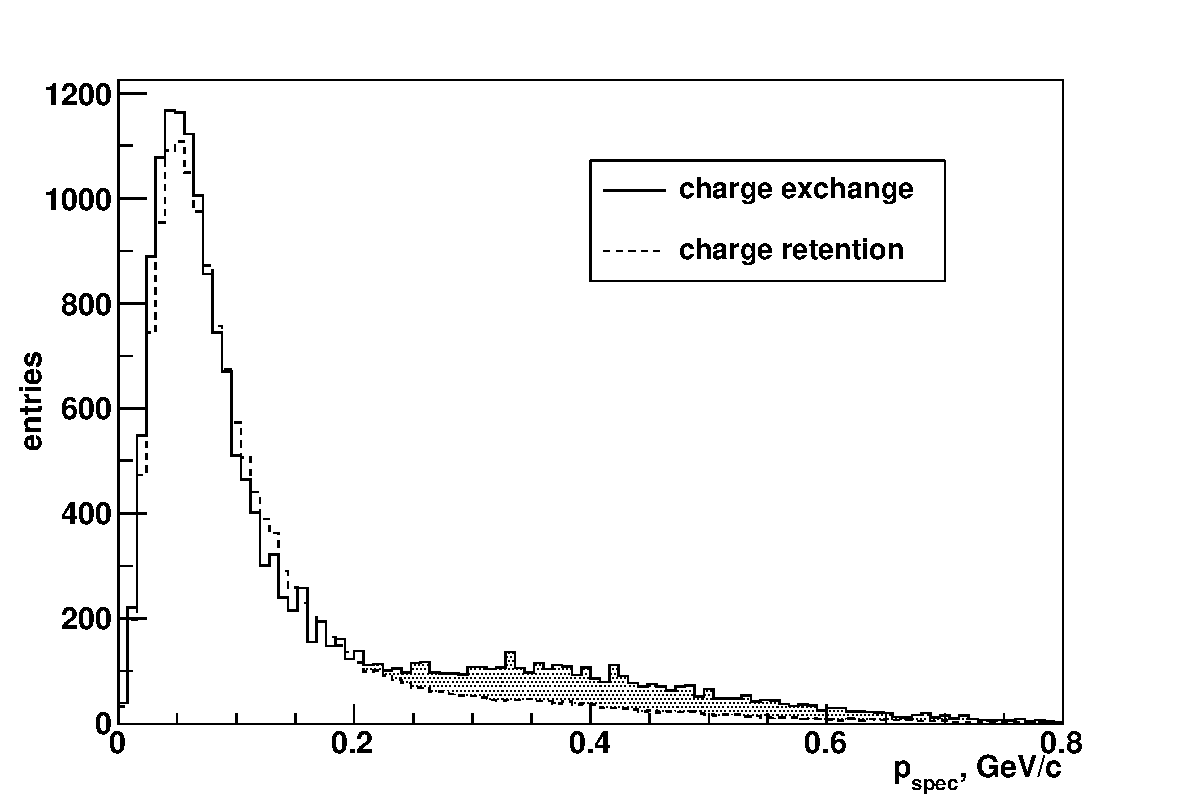
\includegraphics[width=1.00\textwidth]{resonance_spec.pdf}
  \caption{Импульсные распределения нуклонов спектаторов из реакции прямого
    канала (штриховая линия) и перезарядки (сплошная) нормированные на максимум.
    Заштрихованная область ($p_{spec} \gtrsim 0.2$~ГэВ/с) представляет избыток
    событий связанный с образованием промежуточной $\Delta$-изобары.}
  \label{fig:resonance_spec}
\end{figure}

\section{Оценка вклада спин-зависящей части амплитуды
  \maybebm{{\np}} рассеяния}
Проведённый анализ экспериментальных данных по реакции перезарядки дейтрона на
протоне-мишени, даёт возможность получить информацию о спиновой зависимости
обменного $np$-рассеяния назад. Для ответа, на интересующий нас вопрос о вкладе
спин-зависящей части амплитуды элементарного \np процесса, необходимо, как уже
говорилось раньше, кроме измерения дифференциального поперечного сечения
$(d\sigma/dt)_{\dpchex}$ в реакции \dpchex, привлечь и результаты экспериментов
по измерению дифференциального сечения $(d\sigma/dt)_{\np}$ реакции элементарной
перезарядки \np при $|t|=0$.

В разделе~\ref{section:npnp} первой главы было показано, что среди имеющихся в
литературе экспериментальных данных для $np$-рассеяния, измерения сделанные
Бизардом~и~др. на ускорителе Сатурн~\cite{biz75} являются наиболее корректными и
самыми близкими по энергии. На их основе мы получили зависимость
(выражение~\eqref{eq:np0}, стр.~\pageref{eq:np0}) дифференциального поперечного
сечения $(d\sigma/dt)_{\np}$ при $|t|=0$ от импульса нуклона в элементарной
реакции перезарядки \np. Для импульса 1.675~ГэВ/с на нуклон получаем
величину $(d\sigma/dt)_{\np}\,|\,_{t=0} = 54.7 \pm 0.2$~мб/(ГэВ/с)$^{2}$.

Определим теперь на основе наших экспериментальных данных значение
дифференциального поперечного сечения $(d\sigma/dt)_{\dpchex}$ изучаемой реакции
перезарядки на дейтроне \dpchex при $|t|=0$ и импульсе дейтрона 3.35~ГэВ/с. Для
набора пар быстрых протонов, попадающих в конус с раствором меньше
5$^{\,\circ}$, строится распределение сечения с учётом миллибарн-эквивалента
события и поправки, равной отношению полного числа спектаторных нуклонов к числу
спектаторов в выбранном конусе. Полученное распределение сечения
аппроксимируется выражением
\begin{equation}
  \label{eq:exdp}
  d\sigma/dt = p_0\exp(p_1\,t + p_2\,t^2)
\end{equation}
в интервале $t$ од 0 до 0.01 (ГэВ/с)$^2$ и приведено на
рис.~\ref{fig:dp_two_protons}. Экстраполяция к $t=0$ дала значение
$(d\sigma/dt)_{\dpchex}\,|\,_{t=0} = 30.2 \pm 4.1$~мб/(ГэВ/с)$^{2}$. Заметим,
что тем же самым способом (вид функции и интервал аппроксимации) были получены
и сечения элементарной перезарядки нейтрона на протоне.

\begin{figure}[h]
  \centering
  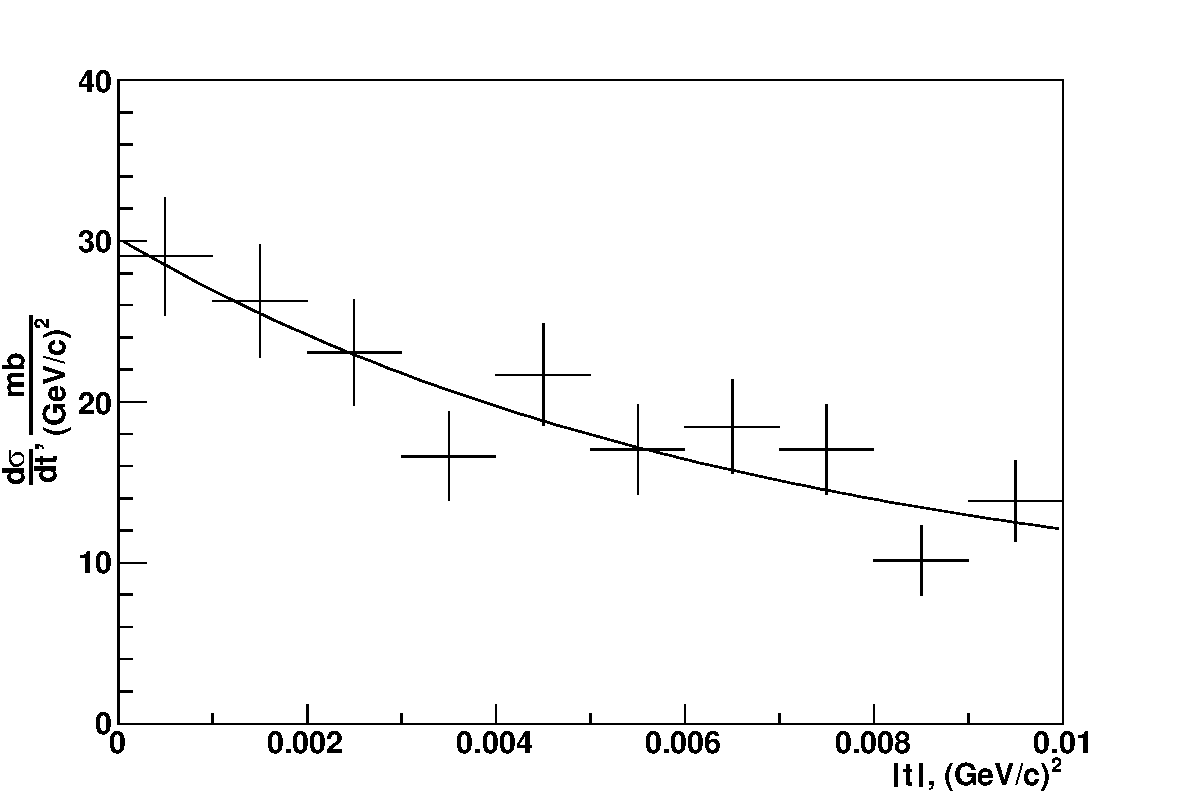
\includegraphics[width=1.00\textwidth]{dp_two_protons.pdf}
  \caption{Распределение дифференциального поперечного сечения реакции с обменом
    заряда \dpchex при малых значениях $|t|$. Сплошная линия~--- аппроксимация
    функцией \eqref{eq:exdp}.}
  \label{fig:dp_two_protons}
\end{figure}

Если бы дифференциальное поперечное сечение перезарядки на дейтроне при $|t|=0$
равнялось точно 2/3 от дифференциального сечения элементарной \np перезарядки
также при $|t|=0$, то это бы означало, согласно выше приведённой
формуле~\eqref{eq:dpnp0}, что амплитуда перезарядки была бы полностью
спин-зависящей. Однако на эксперименте такой закономерности не наблюдается.
Из-за этого было введено отношение $R$, через посредство которого удобно
извлекать долю спин-зависящей (а также и спин-независящей) части амплитуды
реакции \np перезарядки. Величина $R$ используется во многих работах по
интересующей нас теме исследований.

Введём отношение $R_{\np}$ дифференциальных сечений для реакции перезарядки на
дейтроне \dpchex и реакции элементарной перезарядки \np
\begin{equation}
  R_{\np} = \frac{(d\sigma/dt)_{\dpchex}}{(d\sigma/dt)_{\np}}\,.
\end{equation}
При нулевом переданном импульсе $|t|=0$ отношение $R_{\np}$, исходя из
формулы~\eqref{eq:dpnp0}, определяет вклад спин-зависящей части амплитуды
$np$-рассеяния назад, и его можно записать как
\begin{equation}
  R_{\np} = \frac{2}{3}\,\frac{(d\sigma/dt)^{SD}_{\np}}{(d\sigma/dt)_{\np}}\,.
\end{equation}
Из измеренного нами сечения $(d\sigma/dt)_{\dpchex}\,|\,_{t=0} = 30.2 \pm
4.1$~мб/(ГэВ/с)$^{2}$ и сечения $(d\sigma/dt)_{\np}\,|\,_{t=0} = 54.7 \pm
0.2$~мб/(ГэВ/с)$^{2}$ определённого на основе данных Бизардa~и~др. получаем
значение
\begin{equation}
  R_{\np} = 0.55 \pm 0.08\,,
\end{equation}
означающее преобладающий вклад спин-зависящей части амплитуды реакции
перезарядки нейтрона на протоне~\cite{gla_mucha08}.

Исходя из формул~\eqref{eq:np} и \eqref{eq:dpnp0}, отношение $R_{\np}$ может
быть приравнено к
\begin{equation}
  R_{\np} = \frac{2/3\,(d\sigma/dt)^{SD}_{\np}}
  {(d\sigma/dt)^{SI}_{\np} + (d\sigma/dt)^{SD}_{\np}}
\end{equation}
и, соответственно, доля спин-независящей части сечения $R^{\,ID}_{\np}$ реакции
упругой \np перезарядки равна
\begin{equation}
  R^{\,ID}_{\np} = \frac{(d\sigma/dt)^{SI}_{\np}}{(d\sigma/dt)^{SD}_{\np}} =
  \frac{2}{3\,R_{\np}} \ - \ 1 = 0.21 \pm 0.17\,.
\end{equation}

На рис.~\ref{fig:R_np} показана зависимость величины $R_{\np}$ от кинетической
энергии нейтрона в лабораторной системе координат в сравнении с результатами
других экспериментов. Видно, что полученное нами значение находится в согласии,
как с более ранними~\cite{pag88,lehar09}, так и с недавно опубликованными
результатами группы Дельта-Сигма~\cite{shar09} при более высоких энергиях.

\begin{figure}[!h]
  \centering
  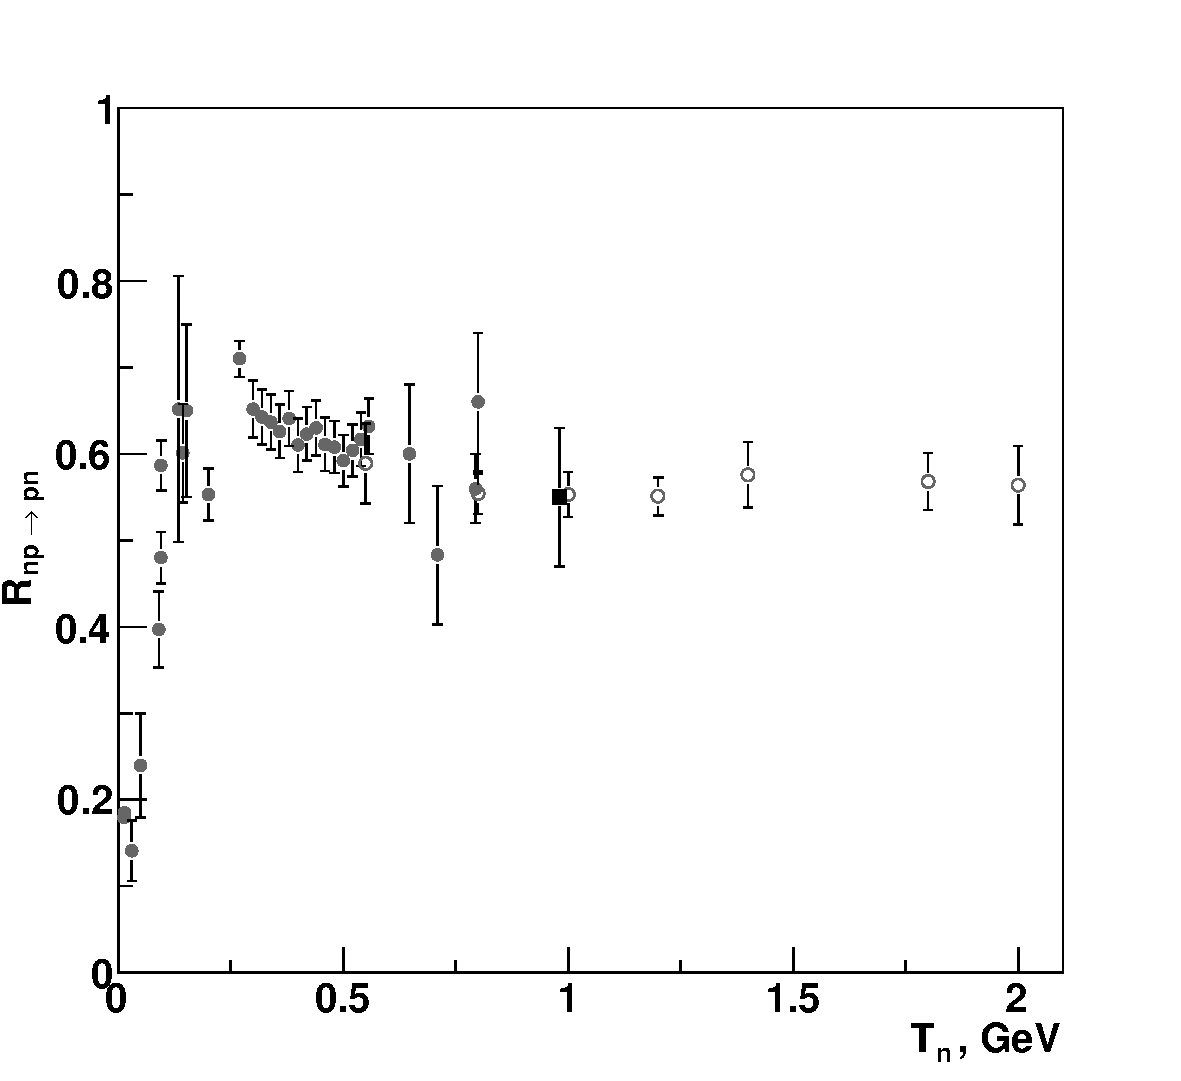
\includegraphics[width=1.00\textwidth]{R_np.pdf}
  \caption{Зависимость величины $R_{\np}$ от кинетической энергии нейтрона
    $T_n$. Сплошные кружки представляют значения полученные в более ранних
    экспериментах, квадратик ($T_n = 0.98$~ГэВ)~--- определённое нами значение
    величины $R_{\np}$, пустые кружки~--- недавно опубликованные результаты
    эксперимента Дельта-Сигма~\cite{shar09}.}
  \label{fig:R_np}
\end{figure}

В работе~\cite{alad75_2} была осуществлена попытка получить экспериментальную
оценку вклада спин-зависящей части амплитуды элементарного \np процесса,
основанную на описании дифференциального поперечного сечения реакции \dpchex,
полученного с помощью водородной камеры через известные к тому времени
экспериментальные данные по $np$-рассеянию. Однако, статистика событий реакции
перезарядки на дейтрона была невелика и данные по $np$-рассеянию были
неоднозначны. Соответственно, и полученная оценка вклада была также
неоднозначна, хотя и указывала на значительную роль зависящей от спина части в
амплитуде \np перезарядки.

В пучке дейтронов это была первая и единственная работа. Следует отметить, что
все более ранние работы на эту тему были проведены в квази-нейтронных вторичных
пучках, получавшихся коллимированными вторичными нейтронами довольно широкого
импульсного спектра. Позже, на эксперименте Дельта-Сигма~\cite{shar09}, где
использовались квази-монохроматические нейтроны от стриппинга выведенных из
ускорителя монохроматических дейтронов, удалось существенно сузить спектр
такого нейтронного пучка.

\section{Выводы ко второй главе}
В итоге выполнения экспериментальной программы, описанной в настоящей главе,
были получены следующие результаты:
\begin{list}{\labelitemi}{\leftmargin=1em}
\item Проведён полный анализ $dp$-взаимодействий, полученных с помощью 100-см
  водородной пузырьковой камеры ЛВЭ ОИЯИ облучённой в пучке дейтронов при
  импульсе 3.35~ГэВ/с.
\item Получены значения сечений 17 каналов $dp$-взаимодействий и оценены потери
  событий. Качество полученной экспериментальной информации свидетельствовало о
  её пригодности для последующего физического анализа.
\item Определено значение миллибарн эквивалента, необходимого для определения
  дифференциального сечения $d\sigma/dt$ реакции с обменом заряда \dpchex при
  $t = 0$.
\item Исследована реакция перезарядки дейтрона на протоне в эксклюзивной
  постановке c целью определения вклада спин-зависящей амплитуды \np перезарядки
  на основе прямого измерения дифференциального сечения $d\sigma/dt$ при $t = 0$
  и обоснована применимость использованного нами подхода. Определено
  дифференциальное сечение реакции перезарядки
  $(d\sigma/dt)_{\dpchex}\,|\,_{t=0} = 30.2 \pm 4.1$~мб/(ГэВ/с)$^{2}$.
\item Впервые в пучке дейтронов получено отношение $R_{\np}$ дифференциальных
  сечений перезарядки при $t=0$ в реакции \dpchex и \np и в рамках импульсного
  приближения получено
  значение $R_{\np} = 0.55\,\pm\,0.08$, что свидетельствует о преобладающем
  вкладе спин-зависящей части амплитуды \np рассеяния и согласуется с данными
  других экспериментов в области близких энергий.
\end{list}

%%% Local Variables:
%%% mode: latex
%%% TeX-master: "musinsky_disser"
%%% coding: utf-8
%%% End:

\chapter{Эксперимент СТРЕЛА}
Результаты, приведённые в предыдущей главе были получены на основе
экспериментальных данных со 100-см водородной пузырьковой камеры. Данная камера,
работавшая в пучках лёгких ядер на синхрофазотроне ЛВЭ ОИЯИ, являлась
одновременно чистой протонной мишенью, и детектором вторичных частиц. С её
помощью было проведено большое число исследований, результаты которых
сформулированы в научных статьях. Часть их легла в основу данной диссертации.

Однако, наряду со многими преимуществами, у камерной методики имелся ряд
недостатков, которые накладывали существенные ограничения на затраты труда и
времени для получения физических результатов на современном уровне.

Пузырьковая камера довольно медленный прибор из-за инерционности механических
процессов, изменяющих давление, необходимых для получения чувствительности
перегретой жидкости. Кроме того, накладывают свои ограничения времена,
необходимые для восстановления давления в жидкости и для срабатывания
регистрирующей аппаратуры. Поэтому неуправляемость прибора не позволяет
организовать электронный триггер для отбора интересующих экспериментатора
событий. В одном цикле ускорения нельзя было получить более одной--двух
стереофотографий рабочего объёма камеры.

Другим явным недостатком камерной методики является большая трудоёмкость
обработки полученных снимков. Процесс обработки стереофотографий с пузырьковой
камеры был очень длительным, из-за чего результаты исследований были иногда
статистически мало обеспечены. Несмотря на введение автоматизации при
обработке снимков, статистика изучаемых процессов существенно отставала от
современных электронных экспериментов. В итоге, для получения статистически
обеспеченных результатов, требовались годы (иногда и десятилетия) упорного труда
коллективов.

\section{Предложение электронного эксперимента}
Изучение реакции перезарядки, проведённое с помощью камерной методики, позволило
предложить схему электронного эксперимента. По мере развития электронных методов
регистрации частиц (и наличия пучка дейтронов) появилась возможность изучения
интересующего нас процесса при использовании выведенного пучка ускоренных
дейтронов на Нуклотроне ЛФВЭ ОИЯИ. В работе~\cite{glagolev96} было впервые
предложено исследование зарядово-обменных процессов в дейтрон-протонных
соударениях на ускорителе Нуклотрон с целью изучения спиновых эффектов в
неполяризованных пучках дейтронов с помощью электронной методики, для получения
статистически обеспеченного результата по определению вклада спин-зависящей
части амплитуды элементарного $np$-рассеяния.

В предлагаемом эксперименте требуется наблюдать события dp-взаимодействий с
вылетом из мишени двух протонов с близкими импульсами в переднем направлении,
т.е. при малых переданных импульсах. В области энергий 1~ГэВ и выше, на момент
формулирования предложения, практически отсутствовали экспериментальные данные
отношения $R_{\np}$ дифференциальных сечений для реакции перезарядки на дейтроне
и реакции элементарной перезарядки нейтрона на протоне.

Нами была предложена~\cite{bush00_mucha,glagolev00_mucha} довольно простая схема
эксперимента (изучается процесс с малой множественностью вторичных частиц и
предсказуемой кинематикой), а именно~--- использование одноплечевого
спектрометра с достаточно узкой апертурой, изображённая на
рис.~\ref{fig:strela_scheme}. Пучок дейтронов падает на мишень, анализирующий
магнит разводит в пространстве вторичные заряженные частицы протоны (или
$\pi$-мезоны) и непровзаимодействовавшие дейтроны. Основным конкурирующим
процессом при выделении реакции перезарядки (двухпротонные события) является
реакция прямого развала дейтрона (однопротонные события), которая в свою очередь
служит дополнительным калибровочным процессом~\cite{are_mucha04}.

\begin{figure}[h]
  \centering
  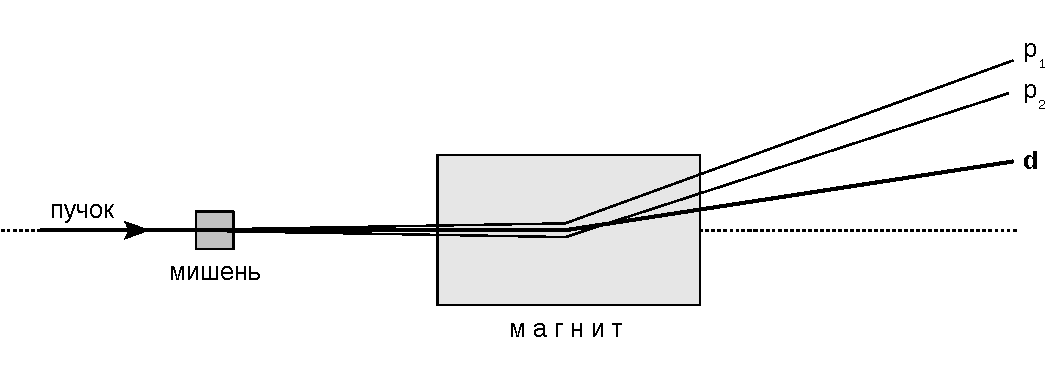
\includegraphics[width=1.00\textwidth]{strela_scheme.pdf}
  \caption{Схема эксперимента с использованием одноплечевого спектрометра,
    обеспечивающая отбор событий с вылетом из мишени двух протонов с близкими
    импульсами в переднем направлении.}
  \label{fig:strela_scheme}
\end{figure}

Предлагаемая \! схема электронного эксперимента позволяет регистрировать пары
протонов с малым углом раствора, имеющие импульс равный приблизительно половине
импульса дейтрона. Этим обеспечивается отбор событий под нулевым углом по
отношению к первичному пучку, что соответствует небольшому переданному импульсу
рассеянному протону ($t \simeq 0$) и малым относительным импульсам внутреннего
движения нуклонов в дейтроне. Таким образом, реализуются необходимые условия для
выделения предполагаемого процесса.

Выбор конкретной геометрии эксперимента был выполнен на основе реальных событий
и расчётов методом генерации Монте"--~Карло с помощью программного пакета GEANT.
Опираясь на данные по реакции $dp \rightarrow X$, полученные на водородной
пузырьковой камере, был промоделирован вариант эксперимента для спектрометра,
используя в качестве входных данных реальные события $dp$-взаимодействий. Для
оценки фоновых условий были взяты все 17 наблюдавшихся каналов реакций
(таблица~\ref{tab:dp_channels}) информация о которых содержится на DST камерного
эксперимента. Фон от других реакций, кроме изучаемой реакции \dpfrag, которые
могли дать два положительно заряженных трека (например
$dp \rightarrow ppn\pi^{0}$) в направлении вперёд при ограниченной апертуре
оказался пренебрежимо малым~\cite{baz99}.

В результате была предложена схема экспериментальной установки
СТРЕЛА~\cite{strela_web}. Были необходимы детекторы с хорошим пространственным
разрешением и быстрая современная электроника для считывания большого потока
информации. В качестве трековых детекторов были выбраны дрейфовые камеры. Не
менее важной задачей был выбор системы отбора и регистрации событий. Особые
требования предъявляются и к характеристикам выведенного из ускорителя и
транспортируемого на мишень пучка дейтронов. Трудности предлагаемой схемы
заключаются в необходимости получения равномерной временной структуры (временная
растяжка пучка в несколько секунд) и ограниченной интенсивности пучка,
фокусируемого на мишень, для уменьшения доли случайных совпадений и минимизации
сбоев в работе дрейфовых камер. В следующих разделах подробно описывается
созданная экспериментальная установка СТРЕЛА.

\section{Описание установки СТРЕЛА}
Экспериментальная установка СТРЕЛА предназначена для исследования
зарядово-обменных процессов во взаимодействиях дейтронов с протонами в области
энергий выше 1~ГэВ. Установка представляет собой одноплечевой магнитный
спектрометр, который расположен в зале корпуса \No205 ЛФВЭ ОИЯИ,
рис.~\ref{fig:strela_205}. Пучок дейтронов, выведенный из ускорителя Нуклотрон,
транспортируется и фокусируется магнитной оптикой канала ВП-1 на мишень
установки, которая находится в области перед фокусом Ф5~\cite{issinsky94}.
Канал транспортировки выведенного пучка состоит из поворотных магнитов и
дублетов магнитных линз, рис.~\ref{fig:channel_VP1}.

\begin{figure}[h]
  \centering
  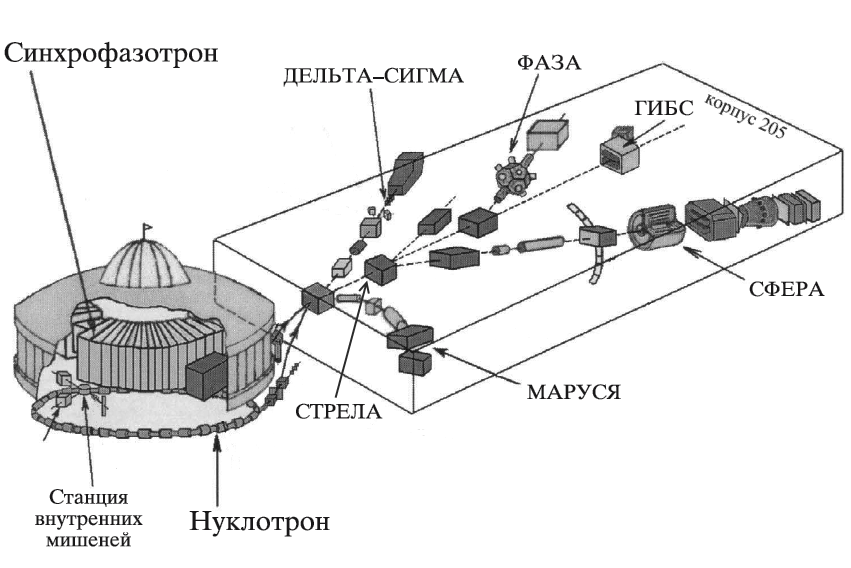
\includegraphics[width=1.00\textwidth]{strela_205.png}
  \caption{Схема ускорительного комплекса ЛФВЭ ОИЯИ Нуклотрон с базовыми
    установками. Установка СТРЕЛА расположена в зале корпуса \No205.}
  \label{fig:strela_205}
\end{figure}

\begin{figure}[h]
  \centering
  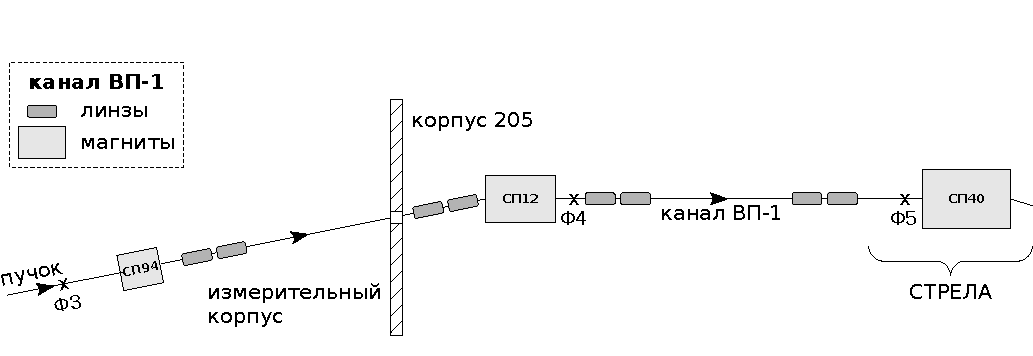
\includegraphics[width=1.00\textwidth]{channel_VP1.pdf}
  \caption{Канал ВП-1 выведенного пучка из ускорителя Нуклотрон с фокусами
    Ф3--Ф5. Транспортировка дейтронного пучка, до мишени установки СТРЕЛА,
    обеспечивается отклоняющими дипольными магнитами и фокусирующими
    квадрупольными линзами.}
  \label{fig:channel_VP1}
\end{figure}

\noindent
Основными элементами установки СТРЕЛА являются:
\begin{itemize}
\item блоки дрейфовых камер в качестве координатных детекторов,
\item электроника считывания информации,
\item сцинтилляционные счётчики используемые для запуска установки,
\item анализирующий магнит.
\end{itemize}

Для определения координат траекторий первичной и вторичных частиц в эксперименте
применяются дрейфовые камеры, которые объединяются в блоки. На
рис.~\ref{fig:strela_setup} приведена схема расположения всех блоков дрейфовых
камер, анализирующего магнита, мишени и сцинтилляционных (триггерных) счётчиков
на выведенном пучке дейтронов из ускорительного комплекса Нуклотрона.

\begin{figure}[h]
  \centering
  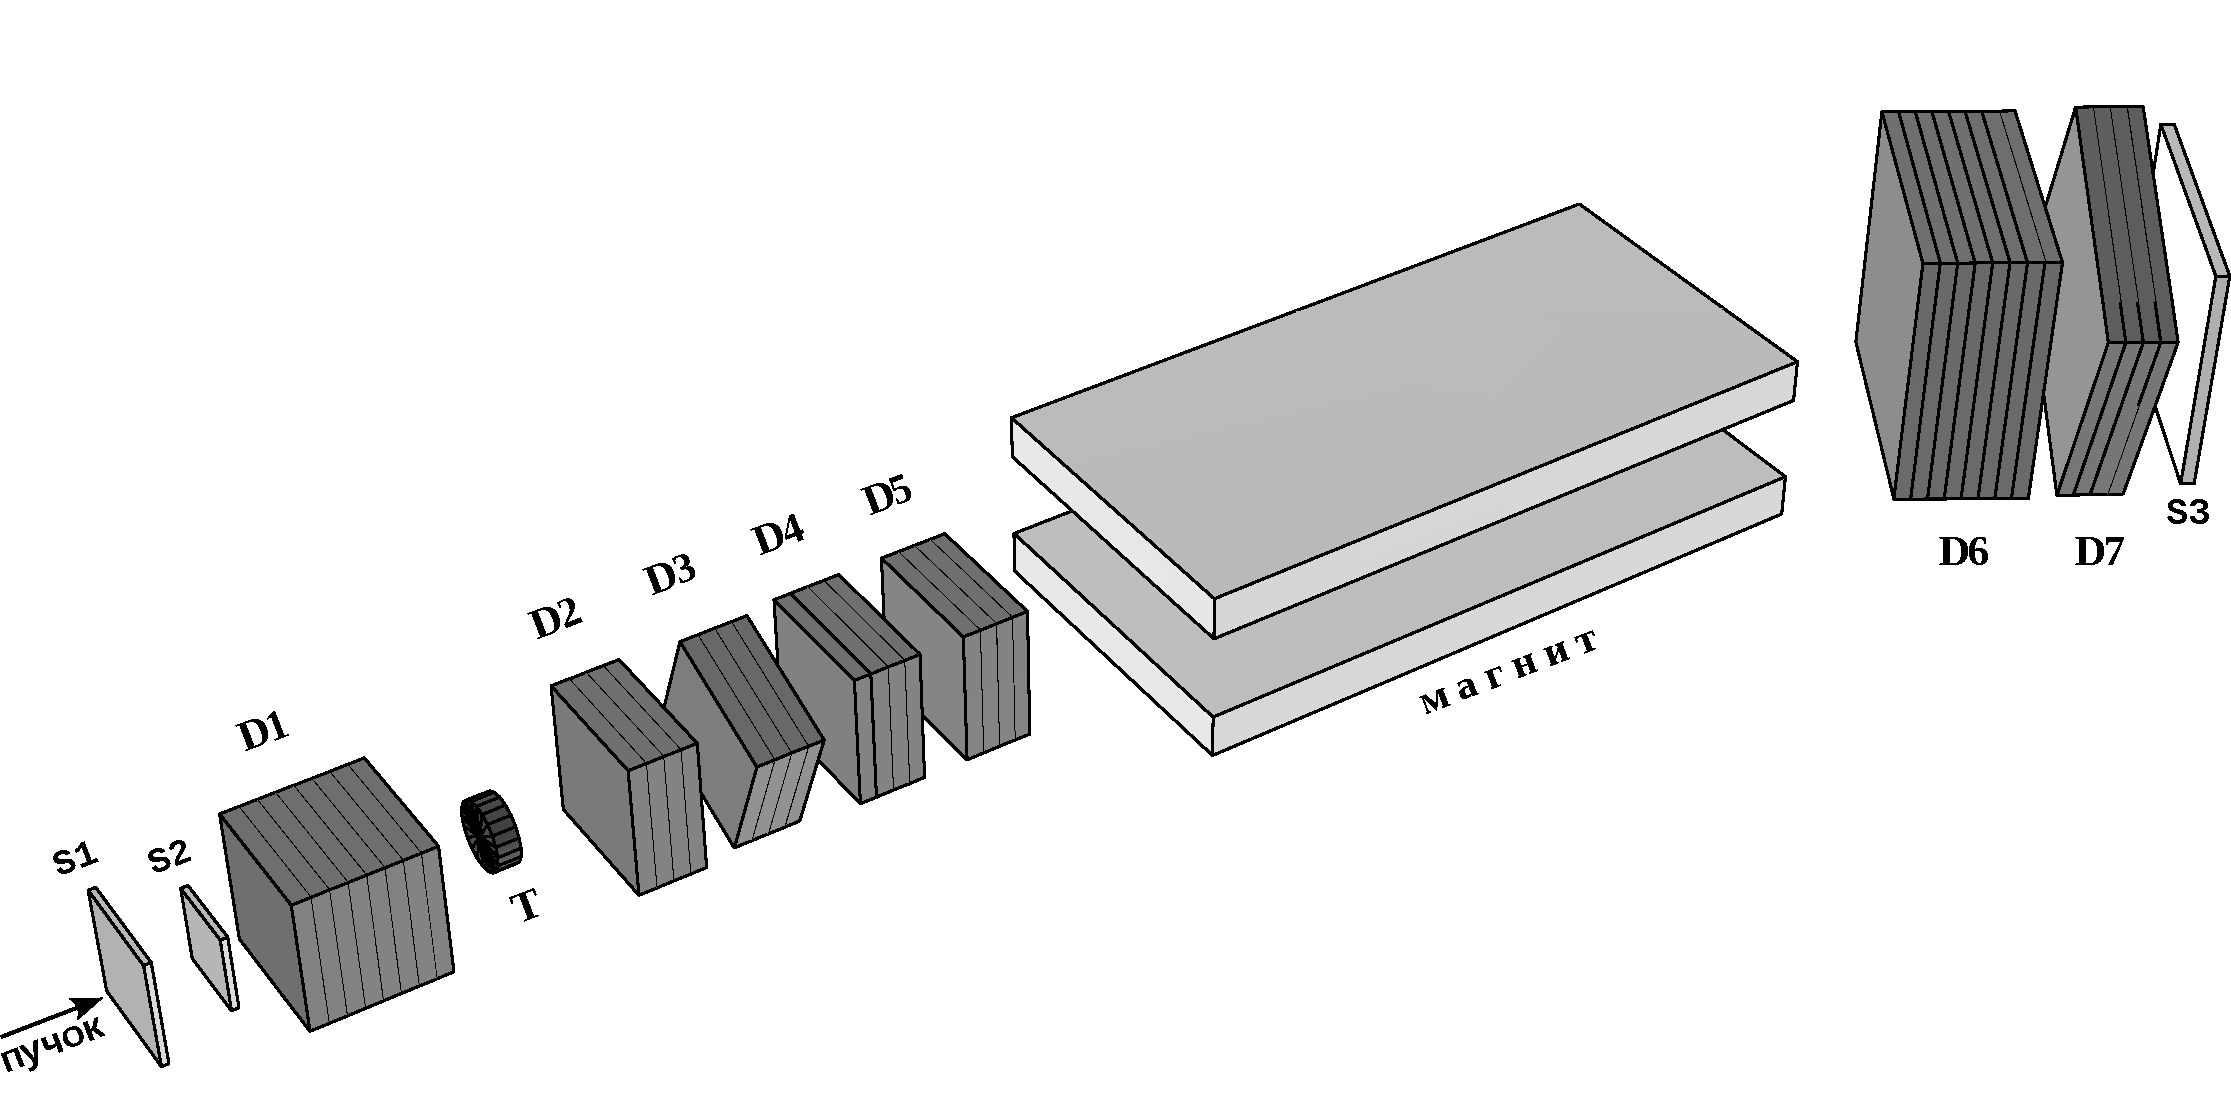
\includegraphics[width=1.00\textwidth]{strela_setup.pdf}
  \caption{Схема расположения дрейфовых камер и анализирующего магнита на
    экспериментальной установке СТРЕЛА. D1--D5~--- блоки <<маленьких>> дрейфовых
    камер с размером рабочей области 12.5~$\times$~12.5~см$^2$, D6--D7~---
    блоки <<больших>> камер с размером 25.0~$\times$~25.0~см$^2$, S1--S3~---
    сцинтилляционные счётчики,  Т~--- мишень.}
  \label{fig:strela_setup}
\end{figure}

В настоящее время используется 36 плоскостей дрейфовых камер, объединённых в 7
блоков. Каждый блок состоит из четырёх или восьми объединённых плоскостей
дрейфовых камер с различной ориентацией проволочек.

Длина дрейфового промежутка во всех камерах равна 21~мм.  Камеры в блоке
располагаются таким образом, что сигнальные проволочки в соседних плоскостях
сдвинуты относительно друг друга на 21~мм в направлении перпендикулярном оси
пучка. Такое расположение нитей позволяет устранить лево-правую неоднозначность
в определении пространственных координат треков частиц.

Координатная система дрейфовых камер выбрана следующим образом: ось $z$ для
блоков камер D1--D5 направлена по пучку падающих дейтронов, а для блоков камер
D6--D7, помещённых после магнита, по направлению максимума вылета протонов
стриппинга; оси $x$ и $y$ лежат в плоскостях камер так, что вместе с осью $z$
составляют правую тройку; координаты $u$ и $v$ используются для повёрнутых камер
вместо $x$ и $y$.

В таблице~\ref{tab:cham_config} приведена структура всех блоков дрейфовых камер
с их регистрируемыми координатами и количеством сигнальных проволочек в каждой
плоскости камеры, штриховая координата используется для сдвинутых проволочек.
\newcolumntype{M}{>{\columncolor[gray]{0.75}[0.90\tabcolsep]}c}
\begin{table}[h]
  \begin{center}
    \bigskip
    \resizebox{1.0\textwidth}{!} {
      \begin{tabular}{|l|c|c|c|c|c|c|c|c|c|c|c|c|c|c|c|c|}
        \hline
        Расположение блока & \multicolumn{16}{c|}{До мишени} \\
        \hline
        Блок & \multicolumn{4}{c|}{} &
        \multicolumn{8}{M|}{D1} & \multicolumn{4}{c|}{} \\
        \cline{6-13}
        Координата & \multicolumn{4}{c|}{} &
        $y$ & $y\,'$ & $y$ & $y\,'$ & $x$ & $x\,'$ & $x$ & $x\,'$ &
        \multicolumn{4}{c|}{} \\
        Число проволочек & \multicolumn{4}{c|}{} &
        4 & 3 & 4 & 3 & 4 & 3 & 4 & 3 & \multicolumn{4}{c|}{} \\
        \hline \hline

        Расположение блока & \multicolumn{16}{c|}{За мишенью} \\
        \hline
        Блок & \multicolumn{4}{M|}{D2} & \multicolumn{4}{M|}{D3} &
        \multicolumn{4}{M|}{D4} & \multicolumn{4}{M|}{D5} \\
        \cline{2-17}
        Координата & $y$ & $y\,'$ & $x$ & $x\,'$ & $u$ & $u\,'$ & $v$ & $v\,'$ &
        $x$ & $x$ & $x\,'$ & $x\,'$ & $y$ & $y\,'$ & $x$ & $x\,'$ \\
        Число проволочек &
        4 & 3 & 4 & 3 & 4 & 3 & 4 & 3 & 4 & 4 & 3 & 3 & 4 & 3 & 4 & 3 \\
        \hline \hline

        Расположение блока & \multicolumn{16}{c|}{За магнитом} \\
        \hline
        Блок & \multicolumn{2}{c|}{} & \multicolumn{8}{M|}{D6} &
        \multicolumn{4}{M|}{D7} & \multicolumn{2}{c|}{} \\
        \cline{4-15}
        Координата & \multicolumn{2}{c|}{} &
        $y$ & $y\,'$ & $y$ & $y\,'$ & $x$ & $x\,'$ & $x$ & $x\,'$ & $u$ & $u\,'$
        & $v$ & $v\,'$ &
        \multicolumn{2}{c|}{} \\
        Число проволочек & \multicolumn{2}{c|}{} &
        7 & 6 & 7 & 6 & 7 & 6 & 7 & 6 & 7 & 6 & 7 & 6 & \multicolumn{2}{c|}{} \\
        \hline
      \end{tabular}
    }
    \smallskip
    \caption{Конфигурация блоков дрейфовых камер на установке
      СТРЕЛА. $uv$-координаты повёрнутые относительно $xy$-координат вокруг оси
      $z$, штриховая координата означает сдвинутую плоскость камеры.}
    \label{tab:cham_config}
  \end{center}
\end{table}



%%% Local Variables:
%%% mode: latex
%%% TeX-master: "../musinsky_disser"
%%% coding: utf-8
%%% End:


До мишени располагается первый блок дрейфовых камер (D1) с размером рабочей
области 12.5~$\times$~12.5~см$^2$, имеющий четыре плоскости $y$-координат и
четыре плоскости $x$-координат. Первый блок служит для определения треков
пучковых дейтронов, падающих на мишень.

За мишенью располагаются четыре блока дрейфовых камер с такими же размерами
(<<маленькие>> камеры). Первый блок (D2) имеет две плоскости $y$-координат и две
плоскости $x$-координат, второй блок (D3)~--- две плоскости $u$-координат и две
плоскости $v$-координат. $uv$-координаты повёрнуты на 22.5$^{\,\circ}$
относительно $xy$-координат вокруг оси $z$, проходящей через центры блоков камер
в направлении падающего пучка. Далее следует блок дрейфовых камер (D4) с
четырьмя плоскостями $x$-координат, и последний блок (D5) имеет две плоскости
$y$-координат и две плоскости $x$-координат. Такой набор камер после мишени
позволяет надёжно идентифицировать два близко проходящих трека. Расстояние между
центрами двух крайних блоков D2 и D5 равно 65~см, между блоком D1 и блоком D2,
расположенными до и за мишенью, равно 90~см.

За анализирующим магнитом располагаются два блока дрейфовых камер с размерами
рабочей области 25.0~$\times$~25.0~см$^2$ (<<большие>> камеры). Ось $z$ данных
блоков (D6--D7) повёрнута на угол приблизительно~14$^{\,\circ}$ относительно оси
$z$ блоков камер (D1--D5), которые расположены перед отклоняющим магнитом.
Первый блок (D6) имеет четыре плоскости $y$-координат и четыре плоскости
$x$-координат, а второй блок (D7)~--- две плоскости $u$-координат и две
плоскости $v$-координат (повёрнутых также на 22.5$^{\,\circ}$ относительно
$xy$-координат). Расстояние между центрами блоков дрейфовых камер D6 и D7 равно
30~см.

Число всех регистрируемых сигналов с проволочек составляет 162. На каждой камере
установлены платы с микросхемами, в которых осуществляется усиление,
формирование и дискриминация входных сигналов от сигнальных проволочек дрейфовых
камер. Сформированные сигналы поступают на входы TDC модулей для оцифровки.
Полученная информация передаётся по оптической линии в персональный компьютер
для дальнейшей обработки.

Дрейфовые камеры являются основным элементом \! экспериментальной установки
СТРЕЛА. Перейдём теперь к более детальному описанию принципов их работы,
конструкции, характеристикам и электронной системе считывания информации с
сигнальных проволочек.

\section{Дрейфовые камеры}
Дрейфовые камеры применяются в физических экспериментах уже почти сорок
лет. Шарпак и его группа впервые предложили идею использовать измерение времени
дрейфа для определения координаты частиц в конце 60-х годов прошлого
века~\cite{charpak68,charpak93}. Дрейфовые камеры стали одним из базовых видов
координатных детекторов на многих установках по физике высоких энергий во всём
мире. Основным преимуществом является высокое пространственное разрешение и
относительно несложная конструкция.

Дрейфовая камера~--- это газонаполненный координатный детектор заряженных
частиц. Координата регистрируемой частицы определяется по времени дрейфа
электронов в газе. Внутри камеры натянуто большое число проволочек, которые
находятся под напряжением. Расположение проволочек выбрано таким образом, чтобы
в пространстве между ними возникало однородное электрическое поле.

Заряженная частица, пролетающая через рабочий объём камеры, оставляет
ионизационный след. Электроны под действием сил электрического поля в камере
движутся с почти постоянной скоростью (дрейфуют) вдоль направления поля к
сигнальным проволочкам, и по достижении ими проволочки, электроника камеры
передаёт на выход сигнальный импульс. По сигналам с проволочек можно с
достаточно хорошей точностью восстановить координаты пролетевшей заряженной
частицы.

\subsection{Ионизация и дрейф электронов в газах}
Основные потери энергии быстрых заряженных частиц происходят в результате
кулоновского взаимодействия при столкновениях с атомными электронами. Заряженная
частица или возбуждает атом, или ионизирует, при этом теряет энергию.
Ионизационные потери энергии на единицу длины пути определяются формулой
Бете"--~Блоха~\cite{pdg08}.

Ионизационное торможение~--- главный механизм потерь энергии при прохождении
быстрой заряженной частицы через вещество детектора. В газовых детекторах, таких
как дрейфовые камеры, вклад от других процессов (тормозное, переходное или
черенковское излучения) в полную потерю энергии частицы незначителен.

Заряженная частица, проходящая через рабочий объём камеры, в результате
ионизации образует электроны и положительные ионы. Они быстро теряют свою
энергию при многократных столкновениях с окружающими атомами и молекулами
рабочего газа, распределение по энергии близко тепловому.

Со временем плотность образованного заряда уменьшается из-за рекомбинации
(нейтрализации положительных и отрицательных ионов) и электронного захвата
(возможности захватывать электроны низких энергий некоторыми многоатомными
молекулами). Вероятность такого захвата характеризуется коэффициентом
прилипания, который для электроотрицательных газов, таких как $O_2$, $CO_2$ и
$Cl_2$, достаточно велик, но пренебрежимо мал для таких газов как $N_2$, $H_2$,
$Ar$ или $CH_4$~\cite{klajk90}.

Если образовавшиеся ионы подвергаются воздействию электрического поля с
напряжённостью $E$, они начинают двигаться вдоль линий электрического
поля. Электроны по направлению поля к анодным проволочкам, а положительные ионы
к катодам. Средняя скорость движения электронов и ионов называется скоростью
дрейфа, её можно записать в виде $v_d = \mu E$, где $\mu$~--- подвижность
ионов, которая кроме напряжённости $E$ в~электрическом поле, зависит также от
состава газовой смеси, давления и температуры. На рис.~\ref{fig:drift_velocity}
показаны зависимости скорости дрейфа электронов от напряжённости электрического
поля для различных газов при нормальных условиях~\cite{sauli02}. Видно, что
скорость дрейфа для разных газов может отличаться на порядок. Кроме того
желательно использовать газ, в котором при достаточной напряжённости
электрического поля, скорость дрейфа слабо меняется при изменении поля.

\vspace{-0.5cm}
\begin{figure}[h]
  \centering
  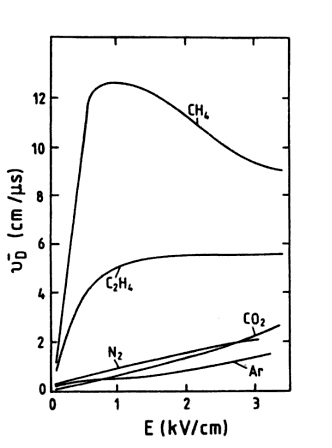
\includegraphics[width=0.55\textwidth]{drift_velocity.png}
  \caption{Зависимость скорости дрейфа электронов $v_d$ от напряжённости
    электрического поля $E$ в некоторых смесях газа при нормальных условиях.}
  \label{fig:drift_velocity}
\end{figure}

Подвижность электронов в газах на несколько порядков больше подвижности ионов
при той же самой напряжённости электрического поля~\cite{pesehonov86}.
Электроны, при достаточно большом значении $E$, смогут за время между двумя
столкновениями, приобрести в электрическом поле энергию, достаточную для
вторичной ионизации атомов газа, произойдёт газовое усиление. В результате число
носителей зарядов возрастает. При высоких значениях $E/p$, где $p$~--- давление
в газе, число новых электронов растёт лавинообразно.

Количество вторичных электронов $\alpha$, образованных в лавине одним электроном
на пути длины 1 см вдоль линии электрического поля, называется первым
коэффициентом Таунсенда, или коэффициентом ударной ионизации. Если $N_0$~---
число первичных электронов, созданных ионизирующей частицей, то полное число
электронов $N(x)$ в точке лавины $x$ равно $N(x) = N_0\,e^{\,\alpha\,x}$.
Коэффициент газового усиления $u$ можно определить как
\begin{equation}
  u\,=\,\frac{N}{N_0}\,=\,e^{\,\int \alpha(x)\,dx}\,.
\end{equation}
На рис.~\ref{fig:gas_townsend} показана зависимость коэффициента Таунсенда от
значения отношения $E/p$. Видно, что развитие лавины в газах, обычно
используемых в дрейфовых камерах, начинается при значении $E/p$ приблизительно
100~В/см~торр~\cite{rope04}.

\begin{figure}[h]
  \centering
  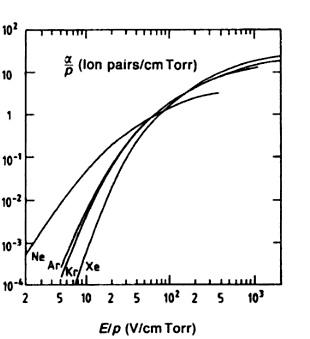
\includegraphics[width=0.55\textwidth]{gas_townsend.png}
  \caption{Зависимость первого коэффициента Таунсенда от значения $E/p$ для
    разных инертных газов.}
  \label{fig:gas_townsend}
\end{figure}

Рабочие газы, используемые в камерах, должны иметь высокий коэффициент газового
усиления. При использовании инертных (благородных) газов, можно получить эффект
газового усиления и при более низкой напряжённости электрического поля. В таких
газах электрон в основном теряет энергию на ионизацию, а не на возбуждение.
В большинстве случаев применяется аргон или ксенон с различными добавками, в
качестве которых чаще всего используется изобутан, метан или
углекислота~\cite{zanevski78}.

Ионизирующая частица, проходящая через дрейфовую камеру, образует вдоль своего
пути свободные электроны, которые зарождают лавины. Заряд рождается в
непосредственной близости от анодной проволочки в области сильного
электрического поля. Сигнал с каждой проволочки регистрируется отдельно, что
позволяет определить координату частицы в камере.

\subsection{Плоская дрейфовая камера}
Идея определения координаты регистрируемой частицы, вызывающей ионизацию газа,
измерением времени дрейфа первичных электронов в однородном электрическом поле,
была высказана уже вскоре после появления многопроволочной пропорциональной
камеры~\cite{charp70}.

Разница во времени $\delta t$ определяется между моментом первичной ионизации
(прохождением частицы) $t_0$ и моментом, когда электроны достигают анодной
проволочки (попаданием облака заряда) $t_1$. Координату $x$ места прохождения
частицы в направлении нормальном к плоскости анодных проволочек в дрейфовой
камере, можно потом вычислить с помощью следующего выражения как
\begin{equation}
  x=\int_{t_0}^{t_1} v_d\,\delta t\,,
\end{equation}
где $v_{d}$~--- скорость дрейфа электронов в газе, которая не должна меняться,
но должна быть достаточно высокой для повышения быстродействия
камеры~\cite{sauli77}.

Для точного измерения координат трековой частицы, необходимо достичь постоянной
скорости дрейфа электронов и линейной зависимости времени дрейфа от координаты
прохождения частицы по всему объёму камеры. Желательную постоянную скорость
дрейфа  можно реализовать созданием постоянной напряжённости электрического поля
вдоль пути дрейфующего электрона. Между соседними сигнальными проволочками
находящимися под потенциалом $+\,U_1$ вводятся дополнительные потенциальные
проволочки под потенциалом $-\,U_2$. На катодные проволочки подан равномерно
распределённый потенциал от 0 до~$-\,U_2$. Данное условие достигается с высокой
точностью практически по всему рабочему объёму дрейфовой камеры, кроме областей
близких к сигнальным проволочкам и на краю камеры, из-за сильного градиента
электрического поля.

Стабильность скорости дрейфа обеспечивается также правильным подбором газовой
смеси. В ряде газовых смесей удаётся обеспечить требуемую скорость дрейфа в
широком диапазоне напряжений~\cite{peisert84}.Тем не менее на изменение
дрейфовой скорости электронов оказывает влияние ряд внешних факторов, таких как
температура, влажность, атмосферное давление или внешнее магнитное поле. Однако
при соблюдении определённых условий можно достичь стабильной работы камер
(постоянную скорость дрейфа электронов) в течение длительного времени
эксперимента.

Пространственное разрешение дрейфовых камер можно выразить как погрешность в
измерении координаты траектории частицы, которая определяется однородностью
электрического поля в области дрейфа. Ограничение на итоговое разрешение вносит
ещё ряд факторов: временное разрешение электроники, неточности при изготовлении
камеры, диффузия электронов во время их дрейфа к аноду, статистическая
флуктуация первичной ионизации в близости анодной проволочки,
рис.~\ref{fig:resolution_cham}~\cite{sitar87}. Кроме того, пространственное
разрешение ухудшается, в зависимости от угла наклона проходящей частицы к
плоскости камеры. Для очень больших наклонов треков оно может упасть почти в
два раза.

\begin{figure}[h]
  \centering
  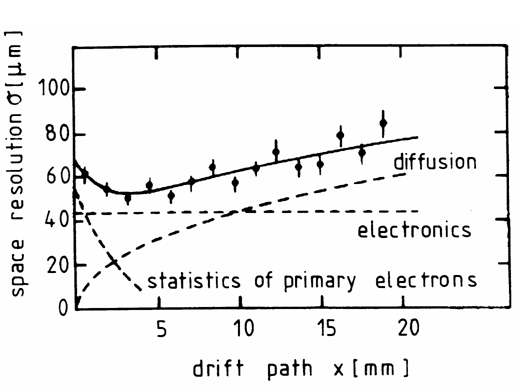
\includegraphics[width=0.80\textwidth]{resolution_cham.png}
  \caption{Пространственное разрешение дрейфовой камеры $\sigma$ в зависимости
    от длины дрейфа электронов $x$.}
  \label{fig:resolution_cham}
\end{figure}

\section{Конструкция дрейфовой камеры}
На экспериментальной установке СТРЕЛА используются два вида дрейфовых камер.
Камеры с размером рабочей области 12.5~$\times$~12.5~см$^2$ (маленькие камеры),
внутри которых натянуты три или четыре сигнальные проволочки, и камеры с
размером 25.0~$\times$~25.0~см$^2$ (большие камеры), имеющие шесть или семь
сигнальных проволочек. Конструкции камер обоих размеров аналогичны.

Одна дрейфовая камера имеет три плоскости проволочных электродов: плоскость
сигнальных и потенциальных проволочек и две плоскости катодов. Принципиальная
схема расположения проволочек дрейфовой камеры показана на
рис.~\ref{fig:cham_wires}.

\begin{figure}[h]
  \centering
  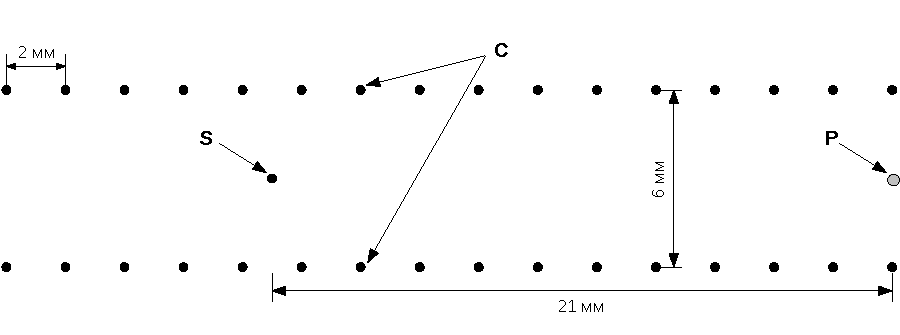
\includegraphics[width=0.95\textwidth]{cham_wires.pdf}
  \caption{Конфигурация проволочек дрейфовой камеры. S~--- сигнальная
    проволочка, P~--- потенциальная проволочка, C~--- катодные проволочки.
    Расстояние между сигнальной и потенциальной проволочками равно 21~мм,
    расстояние между двумя плоскостями катодов 6~мм и шаг намотки между
    катодными проволочками 2~мм.}
  \label{fig:cham_wires}
\end{figure}

Расстояние между двумя соседними сигнальными проволочками равно 42~мм, что
соответствует максимальному дрейфовому промежутку 21~мм. Расстояние между
катодными плоскостями равно 6~мм, шаг намотки катодных электродов 2~мм.
Потенциальные и сигнальные нити, расстояние между которыми 21~мм, расположены в
плоскости, равноотстоящей от катодов~\cite{vodopianov84}.

Для полеобразующих катодных электродов использовалась нить из бериллиевой бронзы
диаметром 100~мкм. Намотка катодных плоскостей проводилась на намоточном станке,
что позволило обеспечить высокую точность укладки проволочек $\pm 15$~мкм.
Сигнальные и потенциальные проволочки, припаянные к соответствующим проводникам
сигнальных и потенциальных печатных электродов, ставились в заданные позиции с
точностью $\pm 10$~мкм под микроскопом. Сигнальные нити~--- золочённая
вольфрамовая проволока диаметром 20~мкм. Потенциальные нити~--- посеребрённая
проволока из бериллиевой бронзы диаметром 60~мкм. Натяжение проволок на уровне
50~грамм~\cite{nigmanov76}.

Расстояние между плоскостью катодных электродов и плоскостью сигнальных и
потенциальных проволочек равно 3~мм. Эквидистантное междуэлектродное
расстояние обеспечивается калибровочными планками, которые приклеены к плоскости
катодных проволочных электродов.

\begin{figure}[h]
  \centering
  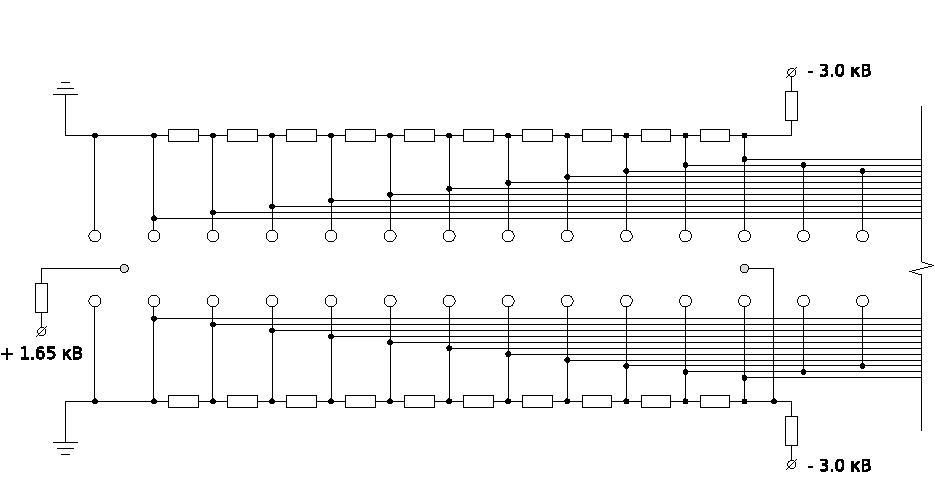
\includegraphics[width=1.0\textwidth]{cham_voltage.pdf}
  \caption{Схема распределения электрического напряжения в дрейфовой камере.
    На сигнальную проволочку подаётся положительный потенциал $+1.65$~кВ, на
    потенциальную $-3.0$~кВ. На катодные проволочки подан равномерно
    распределённый потенциал от $-3.0$~кВ до 0.}
  \label{fig:cham_voltage}
\end{figure}

Распределение напряжённости электрического поля в дрейфовой камере формируется
проволочными электродами. \! Потенциал катодов распределён с помощью резистивных
делителей равномерно от максимального $-3.0$~кВ до нуля. На сигнальные
проволочки подаётся положительный потенциал $+1.65$~кВ, на потенциальные нити
максимальный катодный потенциал $-3.0$~кВ, рис.~\ref{fig:cham_voltage}. Данная
конструкция (в сочетании с газовой смесью) обеспечивает почти постоянную
напряжённость электрического поля $\sim 1.5$~кВ/см вдоль пути дрейфа электронов,
образованных ионизацией среды пролетающей заряженной частицей.

Лево-правая неоднозначность является недостатком при использовании дрейфовых
камер и не позволяет определить, с какой именно стороны пролетела регистрируемая
частица относительно сигнальной проволочки. Неоднозначность устраняется сдвигом
(смещением) соседних плоскостей камер так, чтобы сигнальные проволочки были
сдвинуты относительно друг друга на 21~мм, т.е. на половину расстояния между
ними в направлении перпендикулярном оси пучка. Прямой дрейфовой камерой,
называем камеру имеющую четыре сигнальных и три потенциальных проволочки (для
большой камеры семь сигнальных и шесть потенциальных), сдвинутая камера имеет
три сигнальных и четыре потенциальных проволочки (большая камера шесть
сигнальных и семь потенциальных).

\subsection{Блок дрейфовой камеры}
Блок дрейфовой камеры объединяет несколько плоскостей (слоёв) дрейфовых камер с
различной ориентацией сигнальных проволочек. На установке применяется семь
блоков дрейфовых камер, каждый из которых имеет четыре или восемь плоскостей.
Структура отдельных блоков с их регистрируемыми координатами и числом сигнальных
проволочек указана в таблице~\ref{tab:cham_config}.

На рис.~\ref{fig:cham_block_construct} приведено схематическое изображение
одного блока дрейфовой камеры (показаны только две плоскости камер). Основные
конструктивные элементы блока камеры:
\begin{itemize}
\item рамка камеры,
\item проволочные электроды,
\item печатные электроды.
\end{itemize}

\begin{figure}[h]
  \centering
  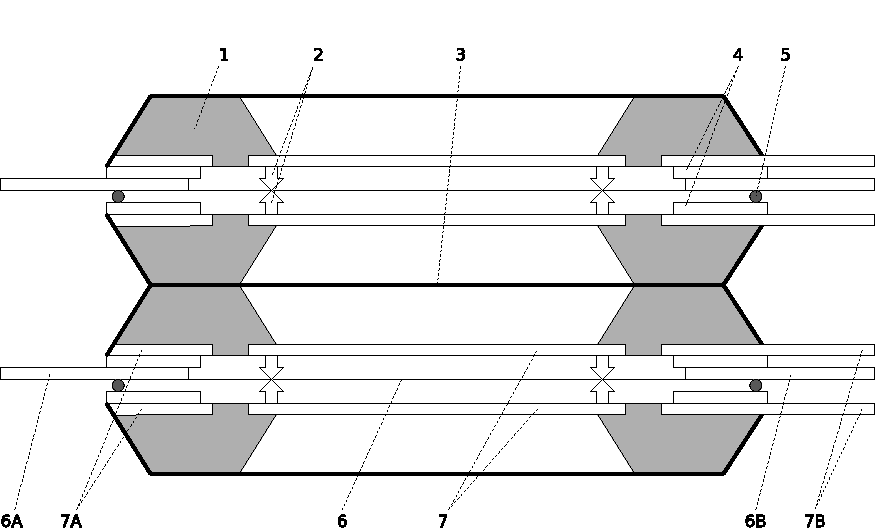
\includegraphics[width=1.00\textwidth]{cham_block_construct.pdf}
  \caption{Изображение одного блока дрейфовой камеры (две плоскости камер).
    1~--- рамка из эпоксидного компаунда, 2~--- калибровочные планки, 3~---
    разделительный проволочный электрод, 4~--- разделительные полосы, 5~---
    уплотняющая резина, 6~--- плоскость сигнальных и потенциальных проволочек,
    6A~--- сигнальный печатный электрод, 6B~--- потенциальный печатный
    электрод, 7~--- плоскости катодных проволочных электродов, 7A и 7B~---
    печатные электроды катодов.}
  \label{fig:cham_block_construct}
\end{figure}

Набор рамок камер из эпоксидного компаунда представляет основной элемент
блока. Технология, принятая при изготовлении, обеспечивает высокую идентичность
механических характеристик всех рамок (размер, коэффициент температурных
изменений и т.п.). С целью повышения необходимой жёсткости рамки армированы
стеклом. Между соседними плоскостями камер установлен разделительный проволочный
электрод. Для герметизации рабочего объёма между отдельными рамками камеры
прокладывается тонкая уплотняющая резина. Расстояние плоскостей сигнальных и
потенциальных проволочек двух соседних камер, объединённых в один блок, равно
26~мм.

Рамки камер одного блока помещаются среди двух внешних алюминиевых рам, которые
имеют каналы для газового обеспечения данного блока дрейфовой камеры. Окна
внешних рам закрыты майларовой плёнкой толщиной 60~мкм. Весь блок дрейфовых
камер, собранный из четырёх плоскостей, имеет толщину 15.4~см, или, для блока из
восьми плоскостей~--- 25.8~см. Плотность вещества в таком блоке дрейфовой
камеры, которая имеет восемь плоскостей, равна 0.141~г/см$^2$~\cite{filatova77}.
Материалы, использованные при изготовлении проволочек, дают основной вклад в
многократное рассеяние. Полная радиационная длина равна $x/X_0 = 0.008$, что
соответствует среднему углу многократного рассеяния для протонов приблизительно
5~мрад.

В каждой рамке камеры находятся отверстия для точной установки печатных
электродов, к проводникам которых припаяны соответствующие проволочки. Все
печатные электроды изготовлены из фольгированного стеклотекстолита. Для создания
одной камеры в блоке используются разные виды электродов~\cite{vodopianov75}.

Потенциальные печатные электроды, предназначенные для подачи максимального
катодного потенциала ($-3.0$~кВ) потенциальным проволочкам, сигнальные
электроды, для подачи положительного потенциала ($+1.65$~кВ) на сигнальные
проволочки. Равномерное распределение катодного потенциала организуется с
помощью резистивных делителей, которые монтируются на катодных печатных
электродах. Съём информации осуществляется с сигнальных печатных электродов.

Все блоки дрейфовых камер находятся в одном общем газовом объёме и продуваются
трёхкомпонентной газовой смесью аргона (72~$\%$), изобутана (25~$\%$) и
этилового спирта (3~$\%$), которая позволяет получить при напряжённости
электрического поля $\sim 1.5$~кВ/см режим постоянной скорости дрейфа
электронов и высокую линейную зависимость времени дрейфа от координаты трека
почти по всему объёму камеры. Замкнутая циркуляционная газовая система
обеспечивает продув каждого блока камер и выдерживает, с достаточной точностью,
стабильность газовых компонент в смеси. Средняя скорость потока смеси в системе
приблизительно 100~см$^{3}$/мин~\cite{filatova77}. С используемой
трёхкомпонентной смесью достигается стабильная работа камер и высокая
эффективность регистрации трековых частиц.

Детекторы установки размещаются на двух отдельных платформах, расположенных до и
после магнита. Блоки дрейфовых камер, расположенные перед анализирующим магнитом
(маленькие камеры), установлены совместно на одной платформе, предназначенной
для закрепления блоков, проведения юстировки, транспортировки и т.п.
Аналогично, камеры находящиеся за магнитом (большие камеры), установлены на
другой платформе.

\section{Электроника считывания информации}
\label{section:electro}
Задача электронной системы регистрации сигналов с анодных проволочек дрейфовых
камер заключается в следующем:

\begin{enumerate}
\item сформирование (усиление, формирование и дискриминация) аналогового сигнала
  с камер,
\item время-цифровое \! преобразование (оцифровка) \! сформированного сигнала в
  модуле TDC (Time Digital Convertor),
\item считывание полученного TDC сигнала и его передача для дальнейшей
  обработки.
\end{enumerate}

Как уже было упомянуто, съём информации с дрейфовых камер осуществляется
с сигнальных печатных электродов, к которым припаяны сигнальные проволочки.
Аналоговая электроника считывания информации с камер для работы в условиях
больших загрузок должна обладать быстродействием для обеспечения высокой
точности и низким уровнем шумов. Для этой цели на камере установлены платы с
двумя специализированными интегральными микросхемами ASD-8~\cite{snowmass99}, на
которые и поступают сигналы с анодных проволочек дрейфовых камер.

Одна микросхема состоит из 8 одинаковых независимых каналов, каждый из которых
содержит быстрый малошумящий усилитель с оптимизированным временем
интегрирования, схемы формирования коротких импульсов и дискриминатор с
управляемым порогом. Все 16 каналов (две микросхемы) используют одно и тоже
напряжение порога. Дифференциальная структура всех звеньев канала была
использована для уменьшения внешних высокочастотных помех и уменьшения наводок
на вход усилителя.

Микросхемы ASD-8 монтируются на многослойных печатных платах размером
6.7~$\times$~5.6~см$^2$. Общее количество каналов равно 16, потребляемая
мощность одного канала не больше 30~мВт, временное разрешение пары импульсов с
камеры лучше 50 нс, напряжение питания $\pm$~3~В и пороговое напряжение
0.5--1.0~В. Для выполнения поверхностного монтажа, на входе и выходе усилителей,
используются миниатюрные многоконтактные разъёмы~\cite{badura00}.

Сформированные импульсы с микросхем передаются по витым парам для оцифровки
на вход время-цифрового преобразователя TDC модуля. Сигналы, поступающие с
проволочек дрейфовых камер и сформированные в микросхемах ASD-8, непрерывно
записываются, с временной точностью 0.1 нс, в буферную память модуля TDC VME при
поступлении тактового сигнала. При появлении триггерного сигнала производится
выборка информации о срабатывании проволочек из буфера, временные параметры
которых находятся в наперёд определённом заданном временном интервале. Этот
интервал определяется максимальным временем дрейфа электронов в камере и
задержкой триггерного сигнала относительно момента прохождения частицы через
установку. Длина временного интервала обычно не превышала 450--500 нс.

В процессе время-цифрового преобразования данные кодируются. Полученная
информация, 32-битовое слово, содержащее номер сработавшего канала (проволочки)
и соответствующее время TDC, считывается по шине VME (Versa Module
Europa)~\cite{smirnov97}. Работа системы сбора тактируется частотой 40 МГц. По
завершении цикла набора данных происходит их передача интерфейсным модулем VME
по высокоскоростной оптической линии в персональный компьютер и запись на
жёсткий диск для дальнейшей обработки.

На установке СТРЕЛА, для организации системы сбора экспериментальных данных
(DAQ), используются несколько модулей быстрой электроники в формате стандарта
VMEbus~\cite{vme85}. Данный стандарт предполагает \! создание
высокопроизводительных вычислительных систем модульного типа на основе
унифицированной магистрали. Он обладает достаточной универсальностью и
расширяемостью. Обмен данными между модулями ведётся по 32-разрядной шине.
Модули размещаются в VME крейте. Упрощённая схема системы сбора данных установки
показана на рис.~\ref{fig:modules_VME.pdf}. Все используемые модули разработаны
и созданы в ЛФВЭ ОИЯИ~\cite{afi_web}.

\begin{figure}[h]
  \centering
  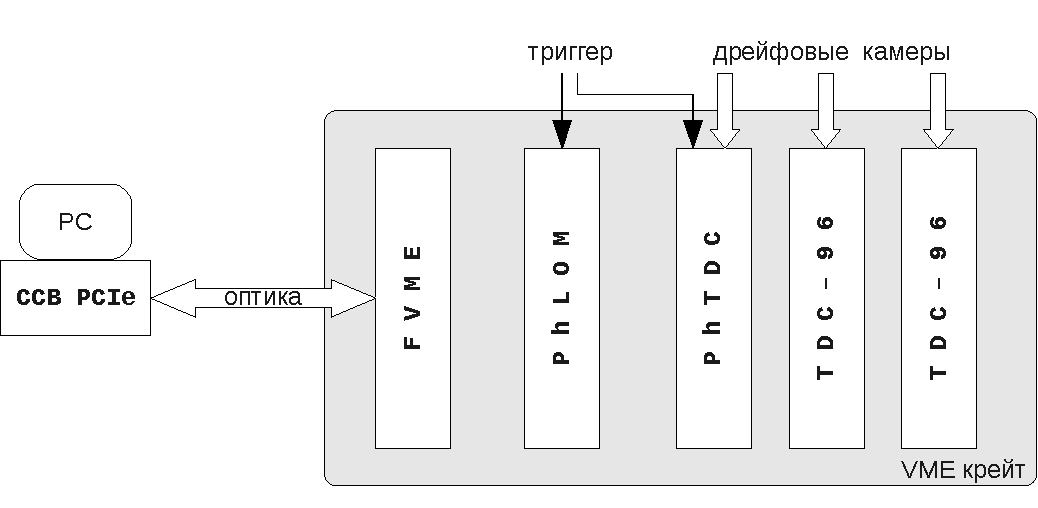
\includegraphics[width=0.95\textwidth]{modules_VME.pdf}
  \caption{Блок-схема системы сбора данных на установке. Сформированные сигналы
    с дрейфовых камер оцифровываются в модулях время-цифрового преобразования
    TDC-96 и PhTDC. Триггерный сигнал поступает на модули PhLOM и
    PhTDC. Интерфейсный FVME контроллер обеспечивает связь VME с удалённым
    компьютером по высокоскоростной оптической линии.}
  \label{fig:modules_VME.pdf}
\end{figure}

Система сбора данных в крейте VME включает в себя разные модули: интерфейсный,
триггерный и TDC. Интерфейсный модуль разработан для передачи данных и
возможности управления системой VME с удалённого компьютера. Контроллер крейта
(тип FVME) соединён по оптической линии с высокоскоростной M-Link сетевой
картой (тип CCB-PCIe) которая вставляется в PCI Express слот компьютера.
Оптическая линия передачи даёт возможность дуплексного обмена данными с большой
скоростью 200~МБ/с на расстоянии до 500 метров при использовании оптического
кабеля.

Триггерный модуль (тип PhLOM) имеет пять логических линий, один тестовый
сигнал, программируемую логику совпадений и счётчики импульсов на входе. Для
системы считывания данных используются выходные сигналы с программируемой
задержкой, которая определяется временем прохождения частицы через установку.
После прихода внешнего триггерного сигнала, в пределах запрограммированного
временного окна, проводится сбор данных по всем каналам.

TDC модули (время-цифровые преобразователи) применяются для преобразования \!
(оцифровки) времени сформированных \! импульсных сигналов с дрейфовых камер. На
данный момент используются три TDC модуля. Один 64-канальный модуль (тип PhTDC)
и два 96-канальные модуля (тип TDC-96). Данные модули разработаны на базе
специализированной интегральной схемы HPTDC~\cite{hptdc04}. Это 32-канальный чип
время-цифрового преобразования с разрешением до 25 пс и оцифровкой обоих фронтов
импульсов.

\section{Система запуска установки, триггер}
\label{section:trigger}
Система запуска установки или отбора событий (триггерная система) в процессе
измерений является необходимой составляющей эксперимента. Триггер установки
СТРЕЛА должен обеспечить набор событий реакции развала дейтрона при нулевом
(близком к нулю) угле рассеяния дейтрона на протоне. В нашем случае
регистрируются два протона с близкими импульсами и малым углом раствора из
реакции перезарядки дейтрона на протоне \dpchex (развал дейтрона с зарядовым
обменом) и однопротонные события из реакции прямого развала дейтрона \dpret.
Доля двухпротонных событий по отношению к однопротонным, при рассеянии на малые
углы, в нашем интервале энергий составляет приблизительно от 10$^{-4}$ до
10$^{-3}$. Однопротонные события~--- это протоны спектаторы и их регистрация
является дополнительным процессом для нормировки дифференциального сечения.

Запуск установки осуществлялся с помощью триггерных счётчиков~--- три
сцинтилляционных счётчика S1--S3 со сцинтилляторами на основе полистирола.
Размеры сцинтилляторов в счётчиках: S1~--- 10~$\times$ 10~$\times$ 0.5~см$^3$,
S2~--- 7~$\times$ 7~$\times$ 0.5~см$^3$ и S3~--- 25~$\times$ 22~$\times$
1.0~см$^3$. Световоды изготовлены из оргстекла. Для считывания света применялись
фотоумножители XP\,2020. Счётчик S3, имеющий сцинтиллятор большой площади,
просматривается двумя ФЭУ для улучшения светосбора и, соответственно, повышения
эффективности регистрации прохождения частиц. Конструкция данного счётчика
показана на рис.~\ref{fig:scintilator_S3}. Счётчики S1 и S2 с одним ФЭУ сделаны
аналогично.

\begin{figure}[h]
  \centering
  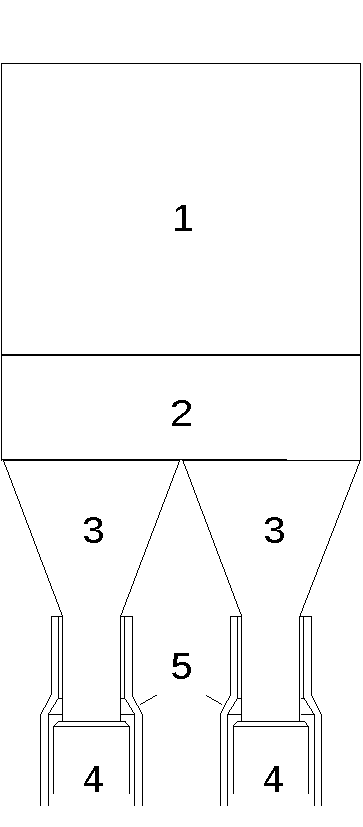
\includegraphics[width=0.32\textwidth]{scintilator_S3.pdf}
  \caption{Конструкция сцинтилляционного счётчика S3 с двумя фотоумножителями.
    1~--- сцинтиллятор (25~$\times$ 22~$\times$ 1.0~см$^3$), 2~и~3~--- световоды
    (оргстекло), 4~--- фотоумножители (XP2020), 5~--- магнитные экраны.}
  \label{fig:scintilator_S3}
\end{figure}

Сцинтилляционные счётчики S1--S3 определяют аксептанс установки и вырабатывают
сигнал для открытия временного окна регистрации сигналов с дрейфовых камер и
запуска системы сбора данных. Сигналы с фотоумножителей
поступают на входы формирователей со следящим порогом. Использование данных
формирователей позволяет скомпенсировать временной разброс сигналов, вызванный
передним фронтом амплитуды сигнала поступающего с ФЭУ. Временная и амплитудная
информация со счётчиков оцифровывается и записывается в каждом событии для
последующего контроля работоспособности счётчиков и всей триггерной системы.

Схема быстрой электронной логики системы запуска считывания данных, используемая
на установке, представлена на рис.~\ref{fig:trigger_scheme}. После
формирователей со следящим порогом логические сигналы поступают на схему
совпадений. В случае совпадения сигналов от всех триггерных счётчиков S1--S3,
вырабатывается сигнал запуска системы считывания данных и событие
регистрируется. Данный триггерный сигнал разветвляется и поступает на вход
триггерного модуля PhLOM VME крейта, на вход модуля TDC VME крейта и на схему
запрета, которая блокирует повторное срабатывание до окончания процесса сбора
данных в контроллер VME крейта. После появления триггерного сигнала проводится
сбор информации (раздел~\ref{section:electro}) по всем каналам дрейфовых камер.

\begin{figure}[h]
  \centering
  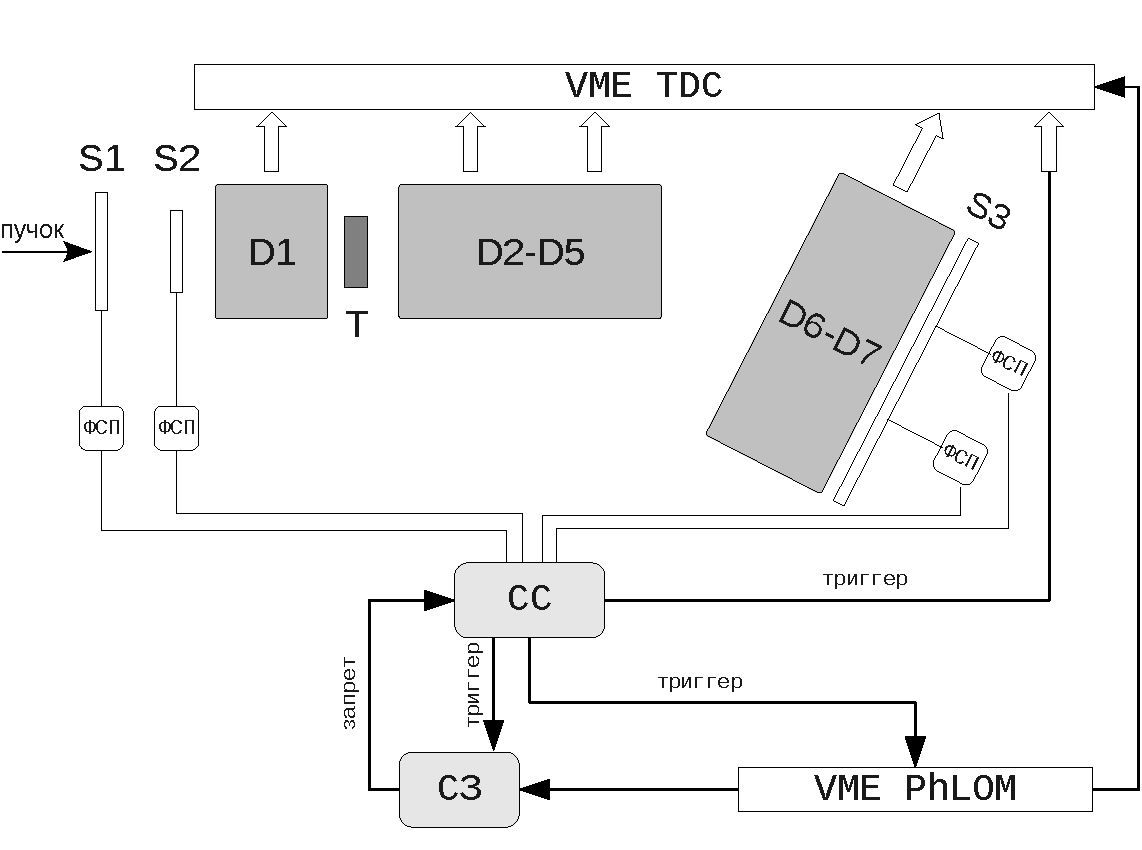
\includegraphics[width=1.00\textwidth]{trigger_scheme.pdf}
  \caption{Схема системы запуска (триггер) считывания данных на установке
    СТРЕЛА. S1--S3~--- сцинтилляционные счётчики, D1--D7~--- блоки дрейфовых
    камер (блоки D6--D7 расположенные после магнита), T~--- мишень, ФСП~---
    формирователь со следящим порогом, СС~--- схема совпадений, СЗ~--- схема
    запрета, VME~TDC~--- модуль время-цифрового преобразования, VME~PhLOM~---
    триггерный модуль.}
  \label{fig:trigger_scheme}
\end{figure}

Во время набора данных, наблюдалась устойчивая работа системы в течение всего
сеанса. Число принимаемых событий за один цикл сброса пучка из ускорителя на
мишень может достигать приблизительно 7500 событий. Среднее число слов, при
регистрации однопротонного события, равно 37 (регистрируемый протон проходит
все 36 плоскостей дрейфовых камер + триггерный сигнал).

Следует отметит, что используемый в данный момент триггер неидеален. Он
обеспечивает приём информации о всех событиях, в том числе и со стриппинговыми
протонами из реакции прямого развала дейтрона, доля которых достаточно велика.
Отбор двухтрековых событий из реакции перезарядки проводится только в процессе
offline обработки, что значительно увеличивает время анализа набранной
информации. Поэтому, желательно было бы организовать специальный триггер, для
отбора двухтрековых событий, используя информацию с дрейфовых камер, однако, это
требует разработки специализированных временных модулей.

\section{Анализирующий магнит}
В качестве анализирующего магнита используется дипольный электромагнит 2СП-40,
расположенный на канале ВП-1 после фокуса Ф5 (рис.~\ref{fig:channel_VP1}) с
поперечными размерами 100~$\times$~30~см$^2$. Магнит создаёт необходимое
магнитное поле в интервале 0.7--1.0~Т на протяжении 150 см, вдоль пути
прохождения частиц. Анализирующий магнит разводит в пространстве
непровзаимодействовавший пучок дейтронов и регистрируемые протоны из реакции
dp-взаимодействия, которые направляются на блоки больших дрейфовых камер.
Радиус кривизны траектории протонов стриппинга в магните равен приблизительно
7~м при значении магнитной индукции 0.83~Т.

\begin{figure}[h]
  \centering
  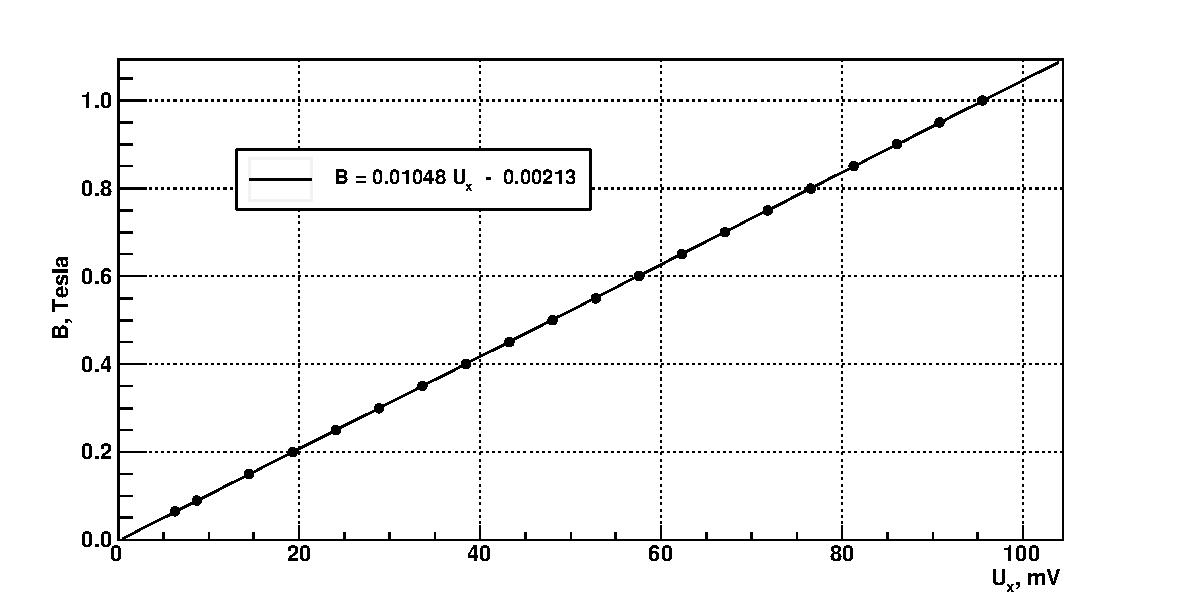
\includegraphics[width=1.00\textwidth]{magnet_hall_calib.pdf}
  \caption{Калибровка датчика Холла ДХ\,10.}
  \label{fig:magnet_hall_calib}
\end{figure}

Контроль и измерение магнитного поля в магните осуществляется датчиком Холла
(модель ДХ\,10), расположенным непосредственно на полюсе электромагнита. Датчик
перед началом измерений был прокалиброван, рис.~\ref{fig:magnet_hall_calib}.
Зависимость между сигналом датчика (холловским выводом) и магнитной индукцией
была строго линейна и аппроксимировалась выражением
\begin{equation}
  B = 0.01048\,U_{x} - 0.00213\,,
\end{equation}
где $B$~--- магнитная индукция в единицах Тесла и $U_{x}$~--- значение выходного
сигнала датчика Холла в мВ.

\begin{figure}[h]
  \centering
  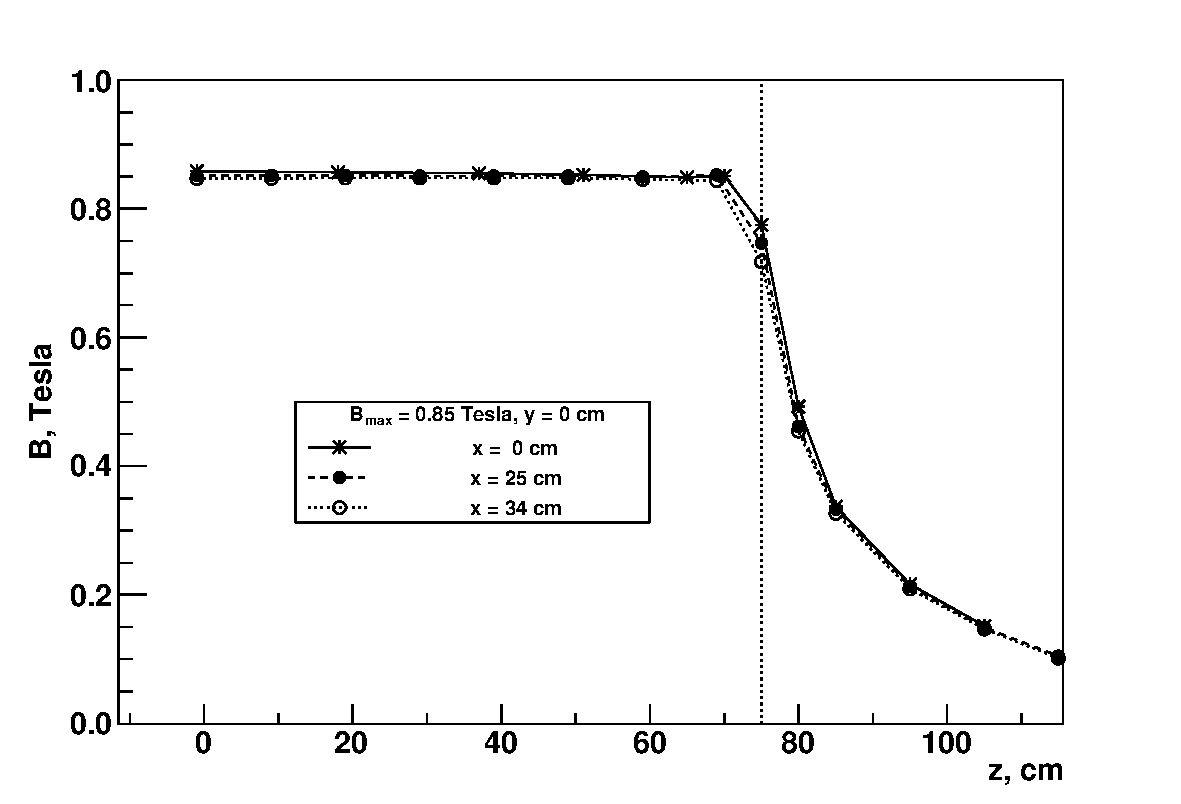
\includegraphics[width=1.00\textwidth]{magnet_eff.pdf}
  \caption{Зависимость магнитного поля $B$ магнита 2СП-40 от $z$-координаты
    для трёх разных значений $x$-координаты в медиальной плоскости $y=0$~см.
    Пунктирная линия означает координату конца полюса магнита ($z=75$~см).}
  \label{fig:magnet_eff}
\end{figure}

Измерения магнитного поля проводились между полюсами магнита 2СП-40 при значении
максимальной индукции в центре магнита 0.85~Т. В медиальной плоскости ($y=0$~см)
снималось по 14 точек вдоль оси $z$ для трёх разных значений $x$-координаты
0~см, 25~см и 34~см. Использовалась такая же координатная система как для
дрейфовых камер (ось $z$ направлена по пучку падающих дейтронов, и вместе с
осями $x$ и $y$ составляют правую тройку). Распределение магнитного поля $B$
вдоль оси $z$ показано на рис.~\ref{fig:magnet_eff}.

Проведённые магнитные измерения показали неоднородность магнитного поля на краях
полюса. Учёт краевых эффектов на полюсах компенсировался увеличением эффективной
длины $L_{eff}$ магнитной дорожки о
\begin{equation}
  \Delta\,L_{eff} = \frac{\int\limits_{L_{1}}^{L_{0}} B(z)\,dz}{B_{max}}\,,
\end{equation}
где $L_{1}$~--- конец области максимального магнитного поля (край полюса
магнита), $L_{0}$~--- конец действия поля и $B_{max}$~--- индукция в центре
магнита. В результате эффективная длина анализирующего магнита 2СП-40 была
увеличена на $\Delta\,L_{eff} = 17.5$~см с каждой стороны (на входе и выходе
частицы в магнит) и составила 185 см. В рабочей области магнита поле оказалось
достаточно однородным. Однако, стоит заметить, что в дальнейшем было бы
желательно провести более точное измерение магнитного поля и составить полную
трёхмерную карту распределения всех компонент вектора магнитного поля.

\section{Облучение аппаратуры СТРЕЛА}
Изучение характеристик всех блоков дрейфовых камер (кроме повёрнутых камер)
экспериментальной установки СТРЕЛА было проведено при облучении полиэтиленовой
мишени диаметром 5~см коллимированным пучком дейтронов с импульсом 3.5~ГэВ/с
на канале ВП-1 ускорительного комплекса Нуклотрона ЛФВЭ ОИЯИ. Сеанс работы
ускорителя состоялся в марте 2007 года. Аппаратура установки проверялась в
течение почти двух суток. Работа повёрнутых блоков дрейфовых камер D3 и D7
(рис.~\ref{fig:strela_setup}), которые были приобретены позже, была
дополнительно испытана с $\beta$-источником.

Система стабилизации интенсивности выведенного пучка из ускорителя обеспечивает
равномерную интенсивность не ниже $\sim 10^{7}$ частиц в секунду. Так как
дрейфовые камеры могут работать при интенсивности не больше $\sim 10^{6}$ частиц
в секунду, то для уменьшения интенсивности использовался стальной коллиматор с
отверстием прямоугольной формы размером 4~$\times$ 4~мм$^2$ и длиной 1.2~м,
устанавливаемый в районе фокуса Ф3 после поворотного магнита СП-94 канала ВП-1
(рис.~\ref{fig:channel_VP1}). Применение коллиматора позволило при интенсивности
пучка в фокусе Ф3 на уровне $\sim 10^{7}$ частиц в секунду обеспечить
интенсивность пучка дейтронов на мишени установки в районе фокуса Ф5 на
уровне $\sim 5 \times 10^{5}$ частиц в секунду.

\vspace{-0.1cm}
\begin{figure}[h]
  \centering
  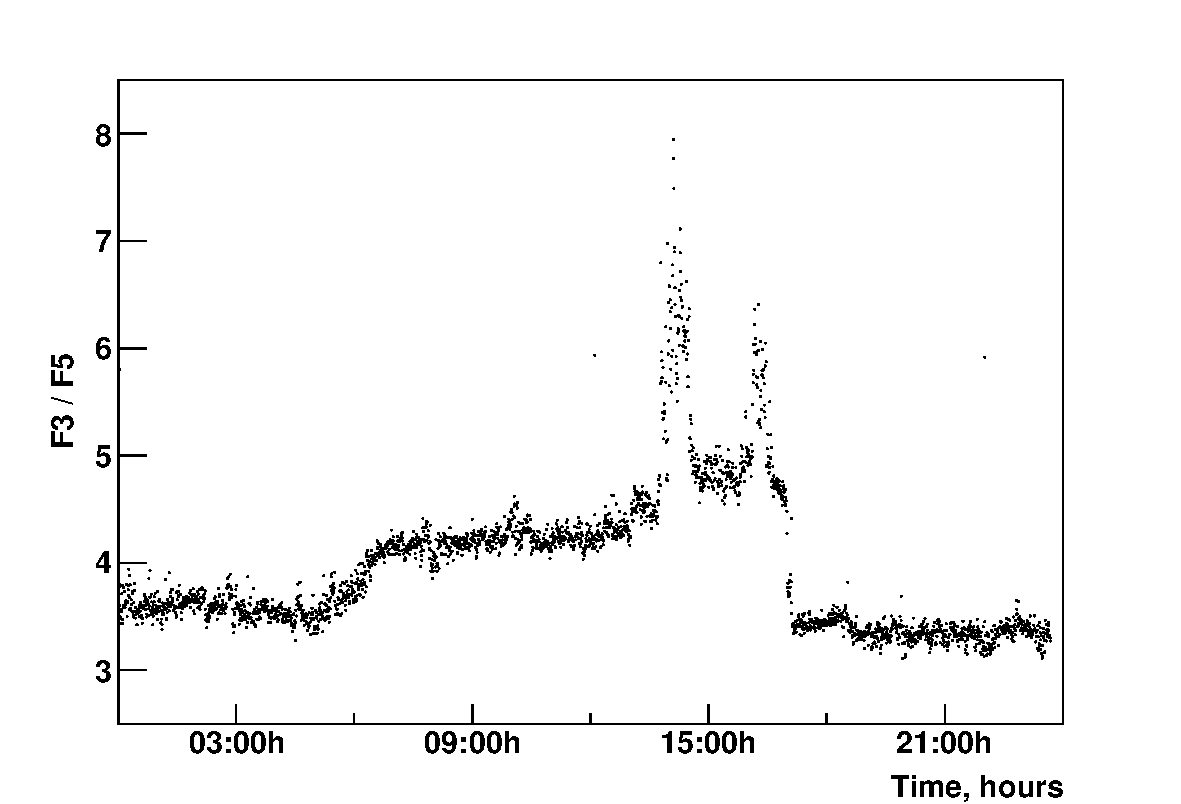
\includegraphics[width=1.00\textwidth]{beam_intensity.pdf}
  \caption{Изменение интенсивности выведенного дейтронного пучка на накале ВП-1
    в течение времени набора данных. Показано отношение счетов ионизационных
    камер, помещённых в фокусе Ф3 и Ф5 в зависимости от времени.}
  \label{fig:beam_intensity}
\end{figure}

Контроль интенсивности выведенного пучка осуществлялся с помощью ионизационных
камер. В процессе набора экспериментальных данных выявились нестабильности
выведенного пучка дейтронов. На рис.~\ref{fig:beam_intensity} приведено
отношение счетов с ионизационных камер расположенных в фокусах Ф3 и Ф5 в
зависимости от времени набора статистики. Повторные выбросы интенсивности пучка
приводили иногда к сбоям работы источников высоковольтного питания дрейфовых
камер. Использование коллиматора косвенно решает и задачу получения лучшей
временной структуры пучка.

В результате облучения аппаратуры установки СТРЕЛА было набрано несколько
миллионов триггеров для последующего анализа. Записанные события сначала
декодировались. Затем происходил поиск и реконструкция треков в дрейфовых
камерах. Более подробное описание процедуры обработки  полученных
экспериментальных данных будет приведено в следующей главе.

\section{Выводы к третьей главе}
Основные выводы данной главы можно сформулировать следующим образом:
\begin{list}{\labelitemi}{\leftmargin=1em}
\item Используя результаты исследований с помощью водородной
  пузырьковой камеры нами был предложен электронный эксперимент СТРЕЛА для
  изучения реакции перезарядки на дейтроне \dpchex с целью определения
  спин-зависящей части амплитуды элементарной перезарядки \np.
\item При активном участии диссертанта была создана экспериментальная установка
  СТРЕЛА и подробно описаны её основные компоненты.
\item Подробно освещены принципы работы и конструкции используемых дрейфовых
  камер, как наиболее важного элемента установки. Проведены испытания всех
  блоков дрейфовых камер и проверена их работа.
\item Обсуждены вопросы считывания информации, системы сбора данных с помощью
  быстрой электроники в формате стандарта VME и запуска установки.
\item Впервые проведено \! облучение установки в пучке релятивистских дейтронов
  импульса 3.5 ГэВ/с на ускорительном комплексе Нуклотрона ЛФВЭ ОИЯИ.
\end{list}

%%% Local Variables:
%%% mode: latex
%%% TeX-master: "musinsky_disser"
%%% coding: utf-8
%%% End:

\chapter{Восстановление треков в дрейфовых камерах}
Выбор дрейфовых камер в качестве координатных детекторов спектрометра на
экспериментальной установке СТРЕЛА обусловлен возможностью получения высокого
пространственного разрешения и более надёжного отбора двух близко проходящих
треков частиц.

Применение дрейфовых камер требует нахождения соотношения между измеренным
временем дрейфа проходящей частицы и его преобразованием в расстояние
относительно данной сигнальной проволочки. Сначала используется <<интегральное>>
преобразование, после чего происходит поиск и реконструкция трека. Для получения
более корректного соотношения между временем дрейфа и расстоянием используется
итеративная процедура автокалибровки.

\section{Время дрейфа, TDC}
Временной спектр TDC одного из каналов показан на рис.~\ref{fig:tdc}.
Минимальное и максимальное время дрейфа ($T_{min},\,T_{max}$) для каждого канала
(проволочки) определяется аппроксимацией его временного спектра функцией
\begin{equation}
  \label{eq:tdc_fit}
  N(t) = p[2] + p[3]\,erfc\,\Biggl[\frac{(t - p[0])}{\sqrt{2}\,p[1]} \Biggr]\,,
\end{equation}
отдельно для минимального времени, $T_{min} = p[0] + p[1]$, и отдельно для
максимального, $T_{max} = p[0]$. $erfc(x)$~--- дополнительная функция
ошибок~\cite{erfc_web}. Параметры $p[2]$ и $p[3]$ можно использовать для
качественной проверки фита. Среднее полное время дрейфа составляет
$\sim$~450~нс.

\begin{figure}[h]
  \centering
  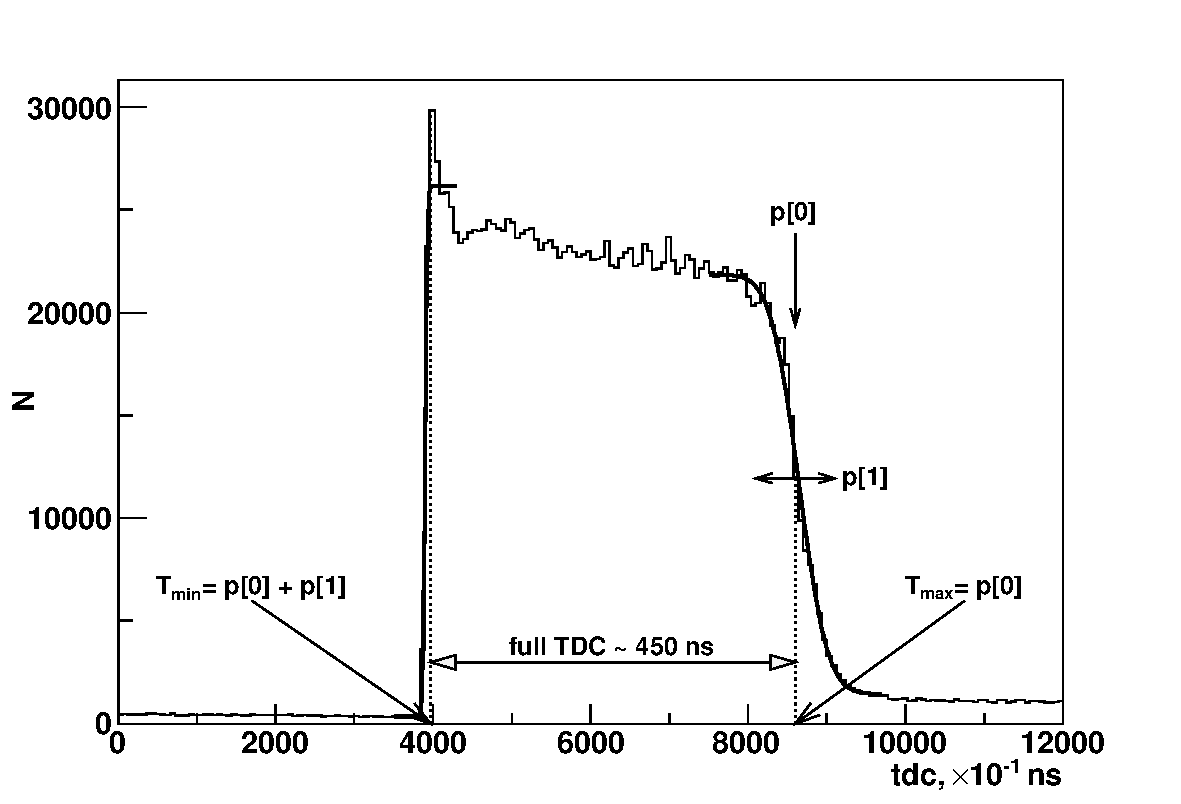
\includegraphics[width=1.00\textwidth]{tdc.pdf}
  \caption{Временной спектр $TDC$ одного из каналов (проволочек) дрейфовой
    камеры. Сплошные линии~--- аппроксимация распределения в области
    минимального $T_{min}$ и максимального $T_{max}$ времени
    функцией~\eqref{eq:tdc_fit}.}
  \label{fig:tdc}
\end{figure}

Соотношение между измеренным временем дрейфа и минимальным расстоянием между
анодной проволочкой и треком частицы имеет важнейшую роль при реконструкции
трека в дрейфовых камерах. Задача состоит в определении функции преобразования
времени дрейфа $t$ в расстояние $r$, так называемое $r(t)$-отношение, зависящее
от многих параметров: напряжённости электрического поля, состава газовой смеси,
давления, температуры, геометрии дрейфовой камеры~\cite{pesehonov86}.

Если предположить, что поток падающих частиц является равномерным, а
эффективность во всей области чувствительности проволочки постоянна, то скорость
дрейфа можно выразить как
\begin{equation}
  v_{d}(t) = \frac{dr}{dt} = \frac{dr}{dN}\,\frac{dN}{dt} =
  const\,\frac{dN}{dt}\,, \qquad
  const = \frac{dr}{dN} = \frac{R}{N_{tot}}\,,
\end{equation}
где $R$~--- длина дрейфового промежутка (21~мм), $N_{tot}$~--- полное число
событий и $dN/dt$~--- временное распределение (рис.~\ref{fig:tdc}).

Таким образом, функцию преобразования времени дрейфа $t$ в расстояние $r$ можно
выразить как
\begin{equation}
  r(t) = \int_{T_{min}}^{T_{max}} v_{d}(t')\,dt' = \frac{R}{N_{tot}}
  \int_{T_{min}}^{T_{max}} \frac{dN}{dt'}\,dt'\,.
\end{equation}
Заметим, что так полученное $r(t)$-отношение (рис.~\ref{fig:t2r}) будет
корректироваться (поправляться) в итеративном процессе
автокалибровки~\cite{gla_mucha10}.

\begin{figure}[h]
  \centering
  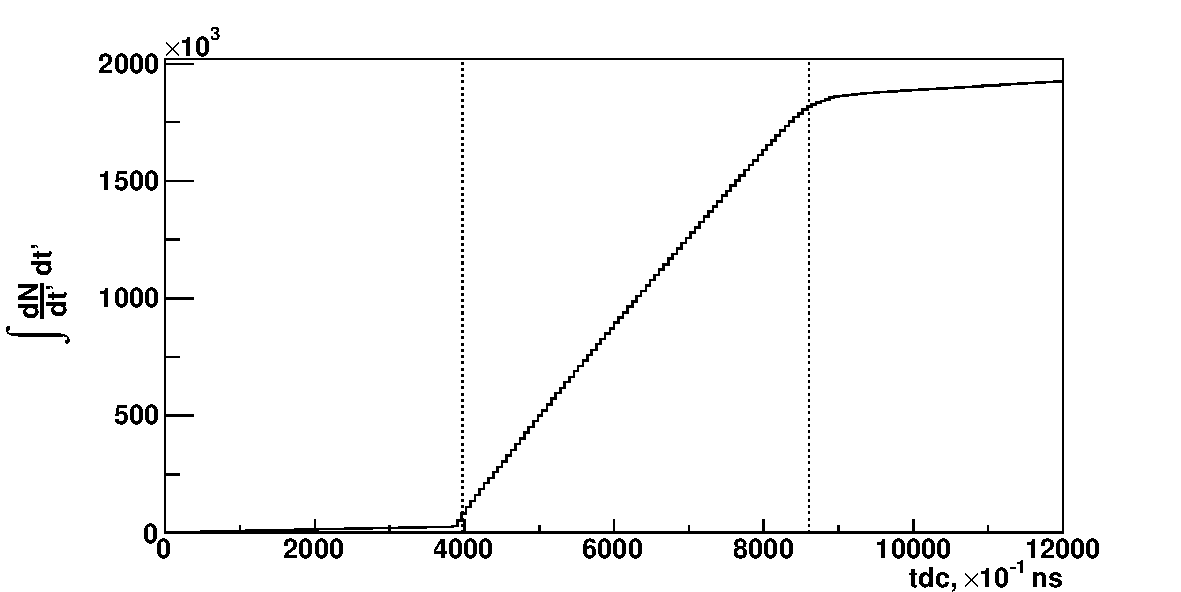
\includegraphics[width=0.965\textwidth]{t2r_t.pdf}
  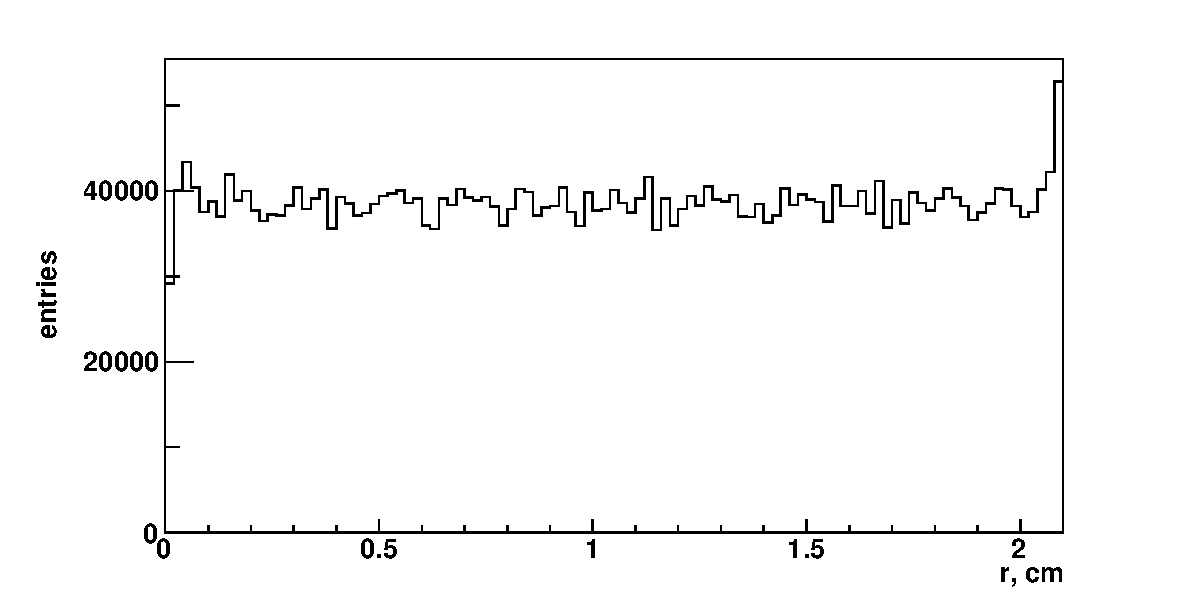
\includegraphics[width=0.965\textwidth]{t2r_r.pdf}
  \caption{На верхнем рисунке интегрированное время дрейфа $t$ проволочки из
    рис~\ref{fig:tdc}. Нижний рисунок~--- преобразованное расстояние $r$ между
    проволочкой и треком.}
  \label{fig:t2r}
\end{figure}

\section{Поиск трека}
Поиск (а позднее и реконструкция) трека происходит отдельно для каждого блока
дрейфовых камер одной плоскости $xz$ или $yz$-координат. В зависимости от
конкретной задачи, можно программным путём, соединять (или разделять) блоки
камер в один мультиблок. В одном блоке (или мультиблоке) должно быть не менее
трёх слоев сигнальных проволочек, для возможности однозначного определения
трека.

\begin{figure}[h]
  \centering
  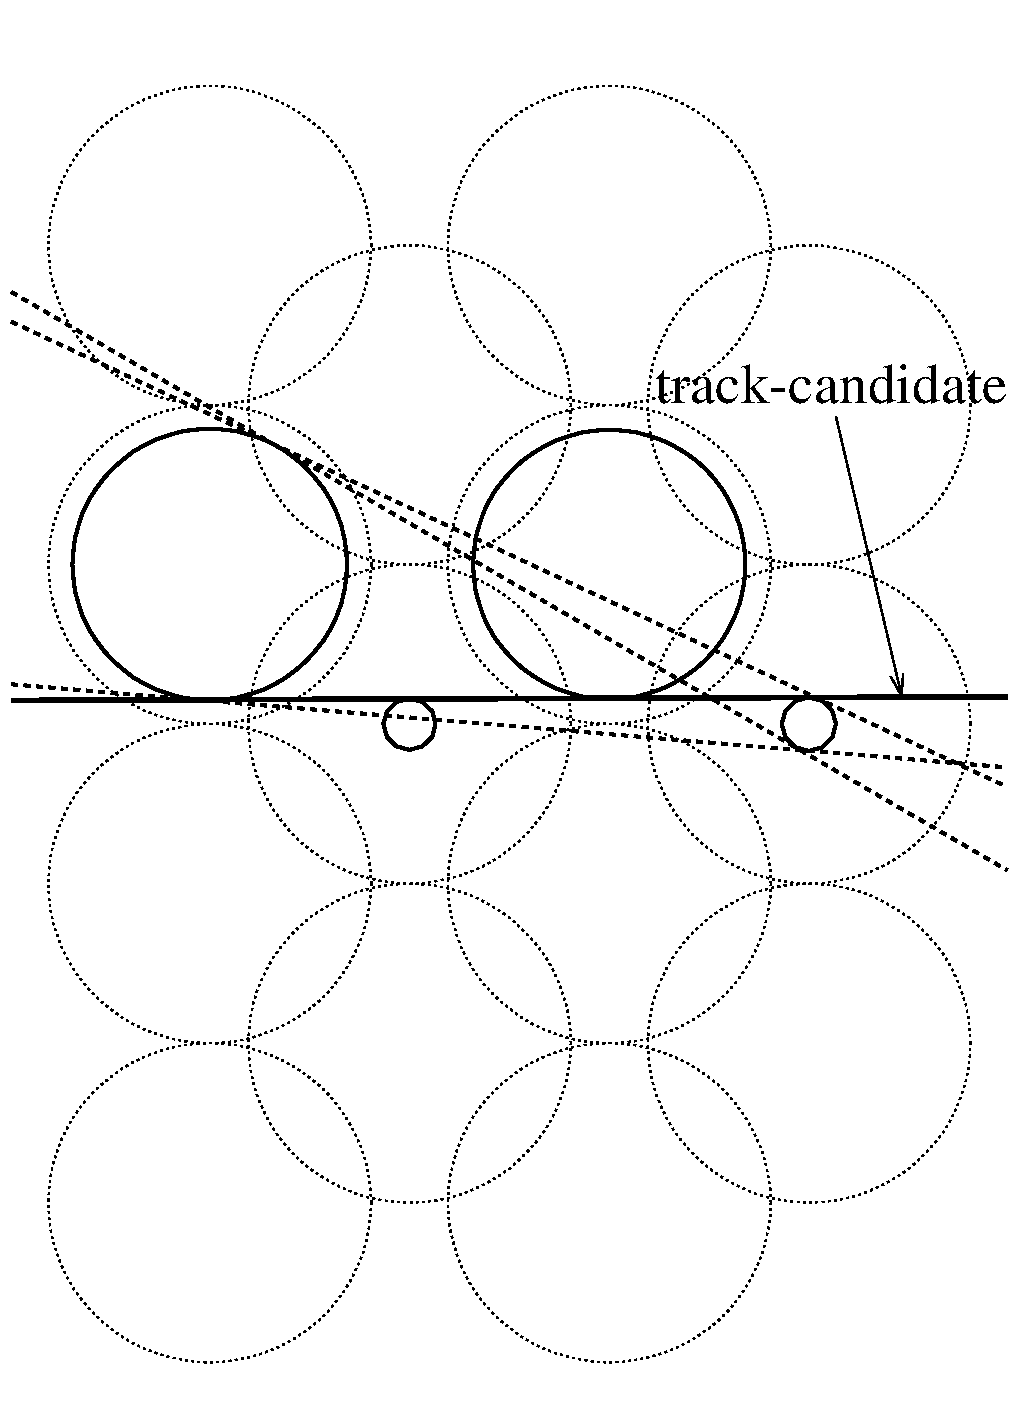
\includegraphics[width=0.48\textwidth]{event_112_run126.pdf} \hfill
  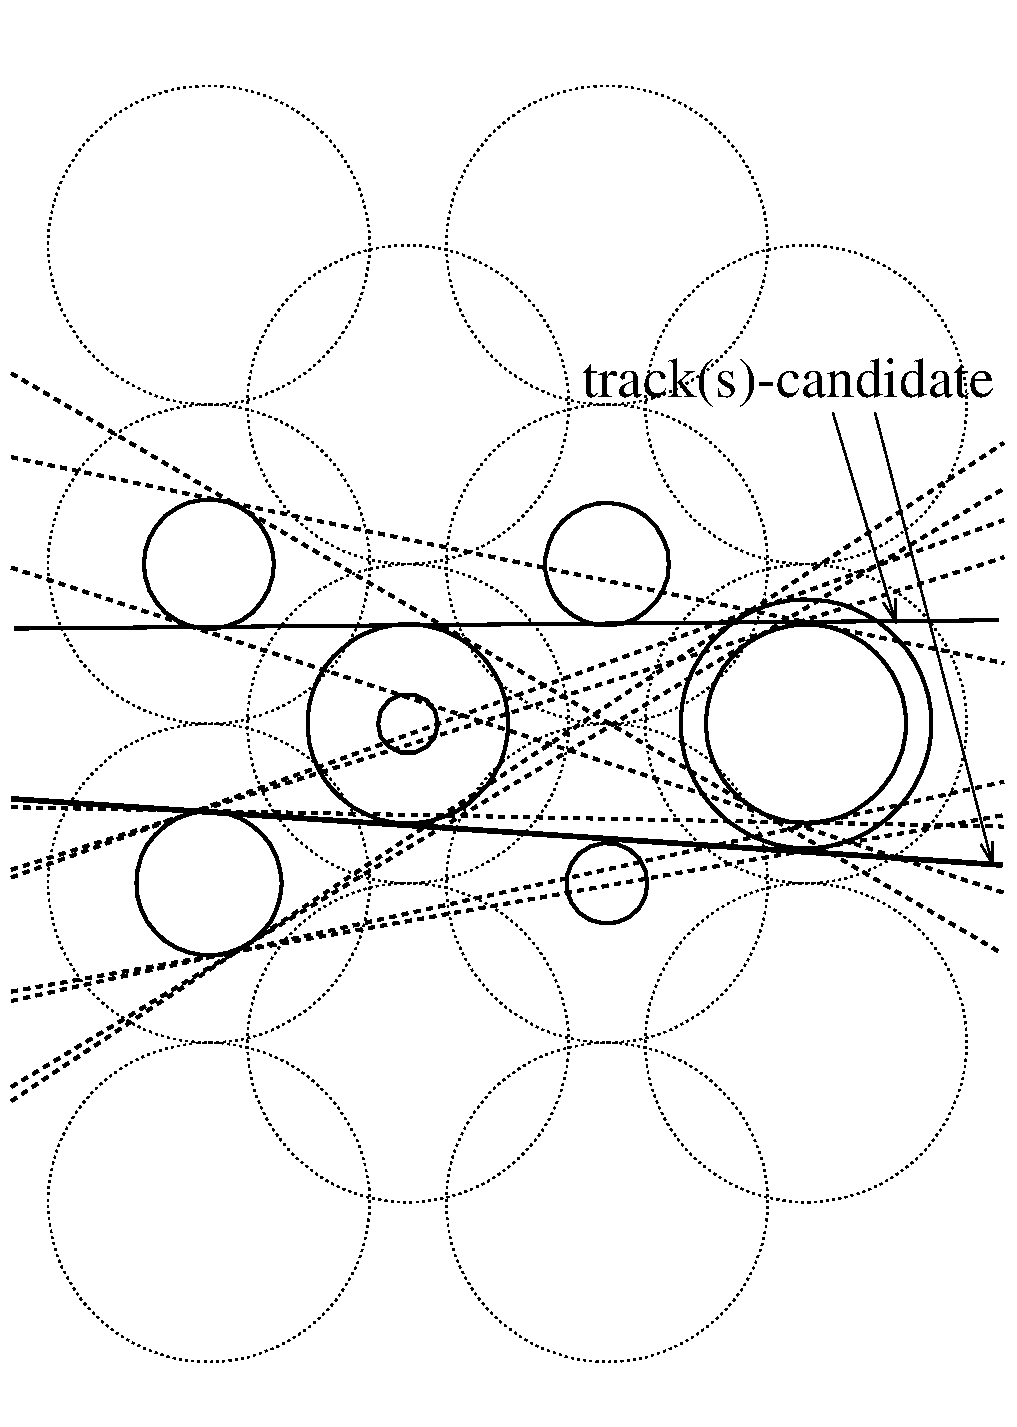
\includegraphics[width=0.48\textwidth]{event_104_run126.pdf}
  \caption{Пример проекции однотрекового (влево) и двухтрекового (вправо)
    события в одной плоскости блока первой дрейфовой камеры, состоящей из
    четырёх слоёв проволочек. Штриховые окружности представляют максимальную
    длину дрейфового промежутка, сплошные~--- расстояние трека от сигнальной
    нити. Для визуального изображения дрейфового промежутка используются
    окружности, центры которых проходят через сигнальные проволочки.}
  \label{fig:typo_2events}
\end{figure}

Последовательность поиска трека в упрощённом виде можно изложить следующим
образом:
\begin{enumerate}
\item Поиск пары сработавших проволочек из разных слоев камеры, имеющих
  наибольшее расстояние. Для пары окружностей, представляющих расстояние
  проекции трека от сигнальной нити, вычисляются параметры всех четырёх
  касательных, рис.~\ref{fig:typo_2events}.
\item Для каждой касательной вычисляется её расстояние $d$ от окружности
  сработавших проволочек. Если расстояние больше, чем заданное минимальное
  $d > d_{min}$, то сработавшая проволочка отбрасывается (не считается).
  $d_{min}$ обычно на порядок больше, чем пространственное разрешение камеры.
\item Если число сработавших проволочек $N_{hits}$ камеры, удовлетворяющих
  предыдущему условию, для касательной не менее заданного
  $N_{hits} \geq  N_{min}$, то касательная переходит в разряд кандидатов в трек.
  Для нашего примера (рис.~\ref{fig:typo_2events}) $N_{min}$ равно 4. Если
  кандидатов несколько, то оставляется тот, у которого сумма расстояний $d$
  минимальна.
\item Производится реконструкция трека и возвращение к 1.~пункту, т.е. поиску
  последующей пары в данном блоке дрейфовой камеры. Сработавшие проволочки,
  которые вошли  в восстановленный трек, не удаляются, и их можно использовать
  для поиска и реконструкции следующего трека.
\end{enumerate}

\section{Реконструкция трека}
Полученный трек-кандидат используется в процедуре реконструкции, восстановления
трека. Проекцию прямого трека в плоскости перпендикулярной к проволочкам блока
дрейфовой камеры можно параметризовать как уравнение прямой
\begin{equation}
  X = aZ + b
\end{equation}
с параметрами $a$ и $b$, рис.~\ref{fig:reco_scheme}.

\begin{figure}[h]
  \centering
  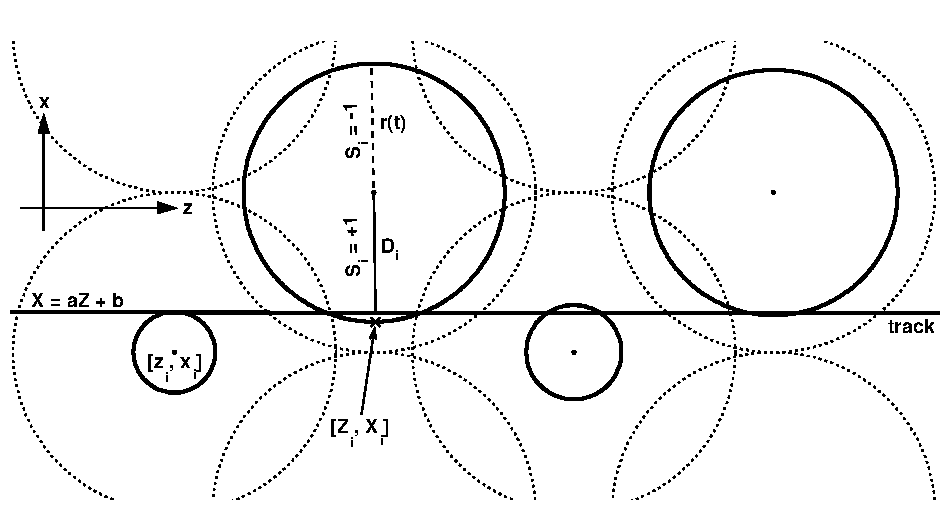
\includegraphics[width=1.00\textwidth]{event_137_run126.pdf}
  \caption{Определение параметров используемых при реконструкции трека в
    блоке дрейфовой камеры.}
  \label{fig:reco_scheme}
\end{figure}

Предположим, что трек имеет $N$ сработавших проволочек с координатами
$(z_i, x_i)$ для $i = 1, \ldots N$. Тогда расстояние между треком и $i$-й
проволочкой можно выразить как
\begin{equation}
  D_i = \frac{a z_i - x_i + b}{\sqrt{1 + a^{2}}}\,.
\end{equation}

Задача реконструкции трека состоит в получении параметров прямой $a$ и $b$
путём минимизации $\chi^2$-функции
\begin{equation}
  \label{eq:chi2_1}
  \chi^2 = \frac{1}{N-2}\sum_{i=1}^{N} [|D_i| -S_ir_i]^2 =
  \frac{1}{N-2}\sum_{i=1}^{N} \biggl[
    \Big|\frac{az_i - x_i + b}{\sqrt{1 + a^2}}\Big| - S_ir_i\biggr]^2\,,
\end{equation}
где $S_i$ имеет в зависимости от положения трека относительно проволочки
значение $\pm{1}$ (рис.~\ref{fig:reco_scheme}), $r_i$~--- расстояние между
треком и $i$-й проволочкой, полученное из функции преобразования времени дрейфа
$t$ в расстояние $r$. Величины параметров $a$ и $b$ получаем решением двух
дифференциальных уравнений
$\frac{\partial \chi^2}{\partial a} = 0$ и
$\frac{\partial \chi^2}{\partial b} = 0$, которые можно решить итеративно.
Уравнение~\eqref{eq:chi2_1} можно переписать следующим образом
\begin{equation}
  \label{eq:chi2_2}
  \chi^2 = \frac{1}{N-2}\sum_{i=1}^{N}
  \biggl[\frac{aZ_i - X_i + b}{\sqrt{1 + a^2}}\biggr]^2\,,
\end{equation}
где координаты проволочек $(z_i, x_i)$ заменяем координатами $(Z_i, X_i)$,
которые вычисляются как
\begin{equation}
  \label{eq:chi2_3}
  Z_i = z_i - S_ir_i \frac{a_0}{\sqrt{1 + a_0^2}}\,, \qquad
  X_i = x_i + S_ir_i \frac{1}{\sqrt{1 + a_0^2}}\,.
\end{equation}

Минимизируя $\chi^2$-функцию (уравнение~\eqref{eq:chi2_2}) методом наименьших
квадратов, получаем значения трековых параметров $a$ и $b$ в виде
\begin{equation}
  a = \frac{-\,\beta + \sqrt{\,\beta^{\,2} + 4\,\alpha^2}}{2\,\alpha}\,, \qquad
  b = S_X - a\,S_Z\,,
\end{equation}
где
\begin{equation}
  \alpha = S_{ZX} - S_Z\,S_X\,, \qquad
  \beta = S_{ZZ} - S_{XX} - S_Z^2 + S_X^2
\end{equation}
и
\begin{equation}
  \begin{split}
    S_Z = \sum_{i=1}^{N} Z_i\,, \qquad
    S_X = \sum_{i=1}^{N} X_i\,, \qquad
    S_{ZX} = \sum_{i=1}^{N} Z_i \, X_i\,, \\
    S_{ZZ} = \sum_{i=1}^{N} Z_i^2\,, \qquad
    S_{XX} = \sum_{i=1}^{N} X_i^2\,. \qquad \qquad \\
  \end{split}
\end{equation}
Величину $a_0$ в итеративном процессе последовательно заменяем новым значением
$a$. В качестве начального значение $a_0$ в уравнении \eqref{eq:chi2_3}
используем параметр $a$ из трека-кандидата (касательной). Для частиц падающих
на камеру под небольшими углами можно принять $a_0 = 0$.

В среднем, после двух--трёх итераций параметры $a$ и $b$ практически не
меняются, и если значение $\chi^2/ndf$ меньше заданного, то трек считаем
восстановленным.

\section{Процедура автокалибровки}
Для реконструкции треков необходимо знать отношение между измеренным временем
дрейфа и его преобразованием в расстояние, поэтому получение правильного
$r(t)$-отношения, является одной из важнейших задач. Итеративную процедуру
определения $r(t)$-отношения с использованием трековой информации называем
автокалибровкой~\cite{bac97,pet05,ame04}.

Отметим, что $r(t)$-отношение, полученное в процессе равномерного облучения
частицами дрейфового промежутка не учитывает неравномерность напряжённости
электрического поля вдоль траектории дрейфа электронов, а это, в свою очередь,
приводит к изменению величины скорости дрейфа, и соответственно, к
дифференциальной нелинейности $r(t)$-отношения. Это возможно в конструкции
используемых дрейфовых камер, где напряжённость электрического поля вдоль
траектории дрейфа задаётся резистивной сборкой, резисторы которой имеет разброс
в несколько процентов.

Однако можно предположить приблизительно одинаковые условия в камере, для
которой выполняется автокалибровка. При необходимости можно программным путём
разделить камеры на меньшие или на группы проволочек, для которых предполагаем
те же самые условия. Иногда поиск и реконструкция трека происходит в одном
блоке (мультиблоке) камер, но процедура автокалибровки проделывается для
каждой камеры отдельно.

\begin{figure}[!h]
  \centering
  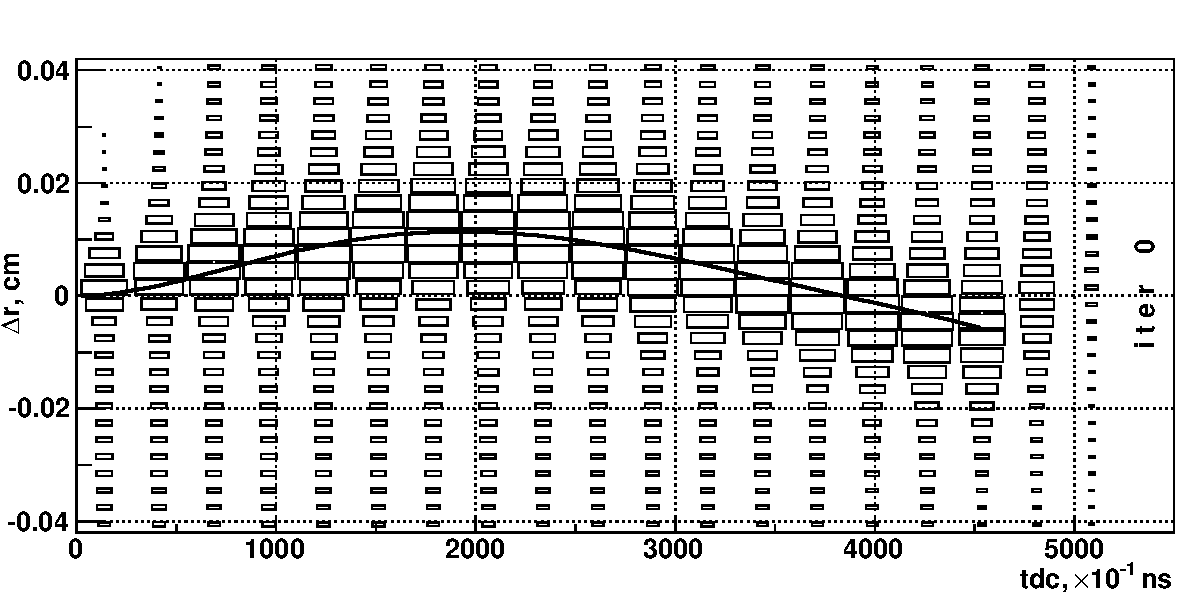
\includegraphics[width=1.00\textwidth]{multi_iter0.pdf}
  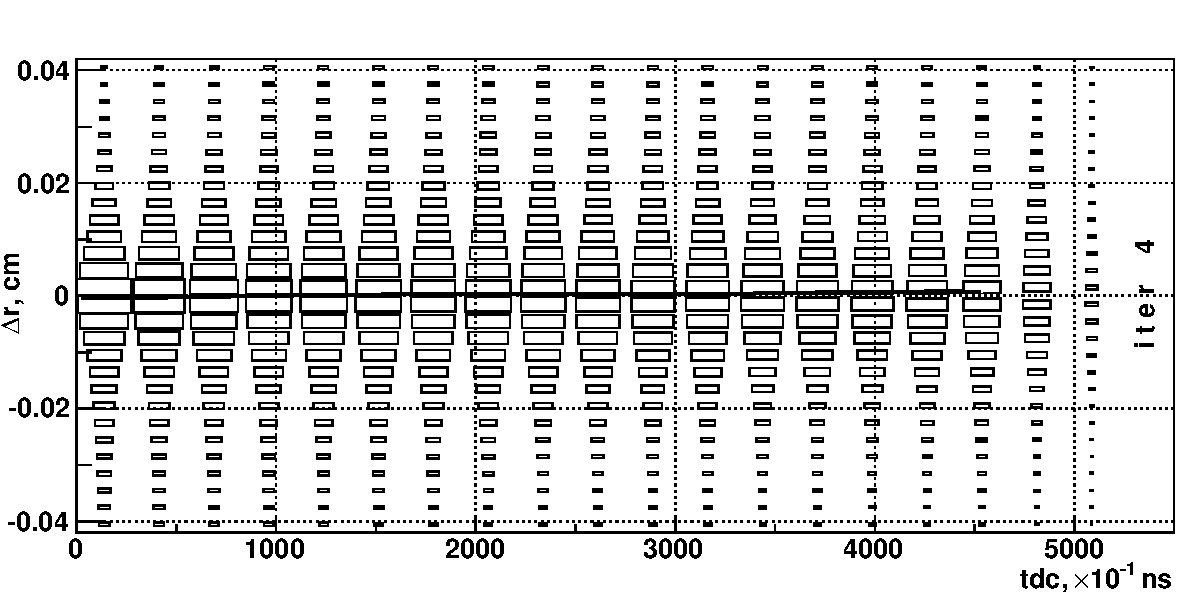
\includegraphics[width=1.00\textwidth]{multi_iter4.pdf}
  \caption{Зависимость распределения трекового остатка $\triangle r$ от времени
    дрейфа $t$ в одной плоскости блока больших дрейфовых камер. Верхний
    рисунок~--- исходное $r(t)$-отношения (интегральное преобразование времени
    в расстояние), нижний рисунок~--- после окончательной, четвёртой итерации
    автокалибровки. Размер прямоугольника пропорционален числу событий. Сплошная
    линия~--- аппроксимация средних значений трекового остатка для каждого
    временного интервала.}
  \label{fig:multi_iter}
\end{figure}

На рис.~\ref{fig:multi_iter} показана зависимость трекового остатка
$\triangle r$ (residual) от времени дрейфа в блоке большой дрейфовой камере.
Трековый остаток можно определить как
\begin{equation}
  \triangle r = r - |D|\,,
\end{equation}
где $r$~--- расстояние полученное преобразованием ($r(t)$-отношение) времени
дрейфа $t$, а $D$~--- расстояние восстановленного трека от проволочки.

Распределение трекового остатка (его ширина) в основном определяется
пространственным разрешением дрейфовой камеры. Тем не менее, $\triangle r$
можно использовать при решении таких задач, как юстирование, сбалансирование
проволочек в блоках (мультиблоках) камер относительно друг друга или для
дополнительной оценки минимального и максимального времени дрейфа. Ожидаемое
среднее значение трекового остатка $\triangle r \simeq 0$.

По горизонтальной оси двумерной зависимости распределения $\triangle r$ от $t$
(рис.~\ref{fig:multi_iter}) отложено время дрейфа с шагом гистограммы 27.5~нс.
Шаг выбран так, чтобы получить необходимое число временных интервалов. В нашем
примере оно равно 20. Для каждого временного интервала создаётся проекция
трекового остатка $\triangle r$. Полученные распределения остатков
аппроксимируются распределением Гаусса, среднее значение которого представляет
поправку $\delta_i$ к текущему $r(t)$-отношению в каждом $i$-м временном
интервале. Таким образом, получается новая, подправленная функция преобразования
времени дрейфа $t$ в расстояние $r$, с которой вновь выполняется реконструкция
трека.

В каждом следующем шаге процедуры автокалибровки $r(t)$-отно\-шение поправляется
в зависимости от предыдущей итерации. Поиск и реконструкция треков проводится
повторно до тех пор, пока значения поправок $\delta_i$ для всех временных
интервалов стабилизируются (приблизятся к нулевым значениям). В нашем примере
число итераций равно 4--5. Как меняется распределение трекового остатка в
зависимости от номера итерации, показано на рис.~\ref{fig:per_iterative}.
Видно, что с ростом номера итерации трековый остаток стремится к нулю, а ширина
распределения уменьшается.

\begin{figure}[h]
  \centering
  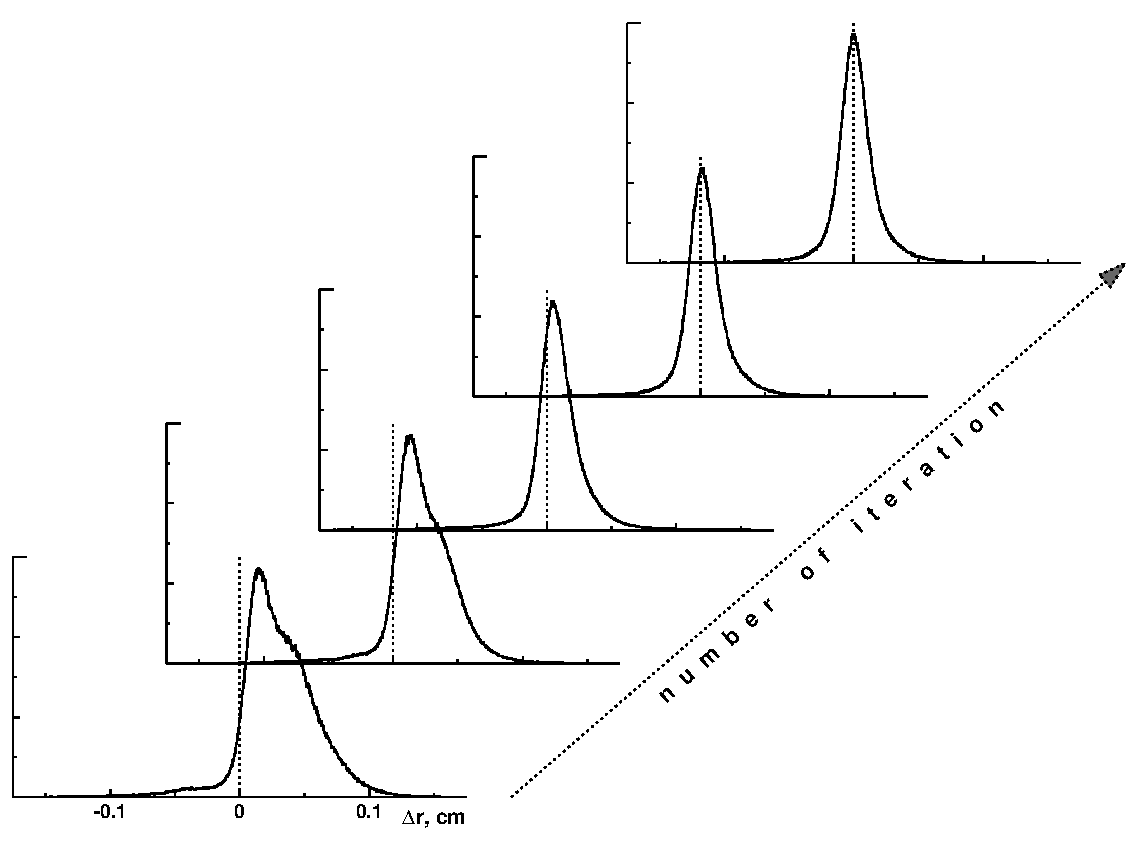
\includegraphics[width=1.00\textwidth]{c_per_iterative.pdf}
  \caption{Изменение распределения трекового остатка $\triangle r$ в зависимости
    от номера итерации в блоке больших дрейфовых камер.}
  \label{fig:per_iterative}
\end{figure}

Процесс автокалибровки выполняется только с однотрековыми событиями. Желательно,
чтобы угловой разброс треков в камере не превышал $\sim$~100~мрад. Если диапазон
наклонов треков, проходящих через камеру, большой, то итеративную процедуру
автокалибровки делаем отдельно для разных диапазонов углов наклона. Область
изменения угла наклона не должна превышать
$\sim$~100--150~мрад~\cite{gla_mucha08_2}.

Пространственное разрешение дрейфовой камеры определяется шириной распределения
трекового остатка данной камеры. Для вычисления разрешения $\sigma$
использовалась аппроксимация двойным распределением Гаусса,
рис.~\ref{fig:res_chambers}. Пространственное разрешение дрейфовых камер,
используемых на установке СТРЕЛА, лежит в диапазоне $\sim$~90--120~мкм.
Влиянием многократного рассеяния (дейтроны с импульсом 3.5 ГэВ/с) на разрешение
можно пренебречь.

\begin{figure}[!h]
  \centering
  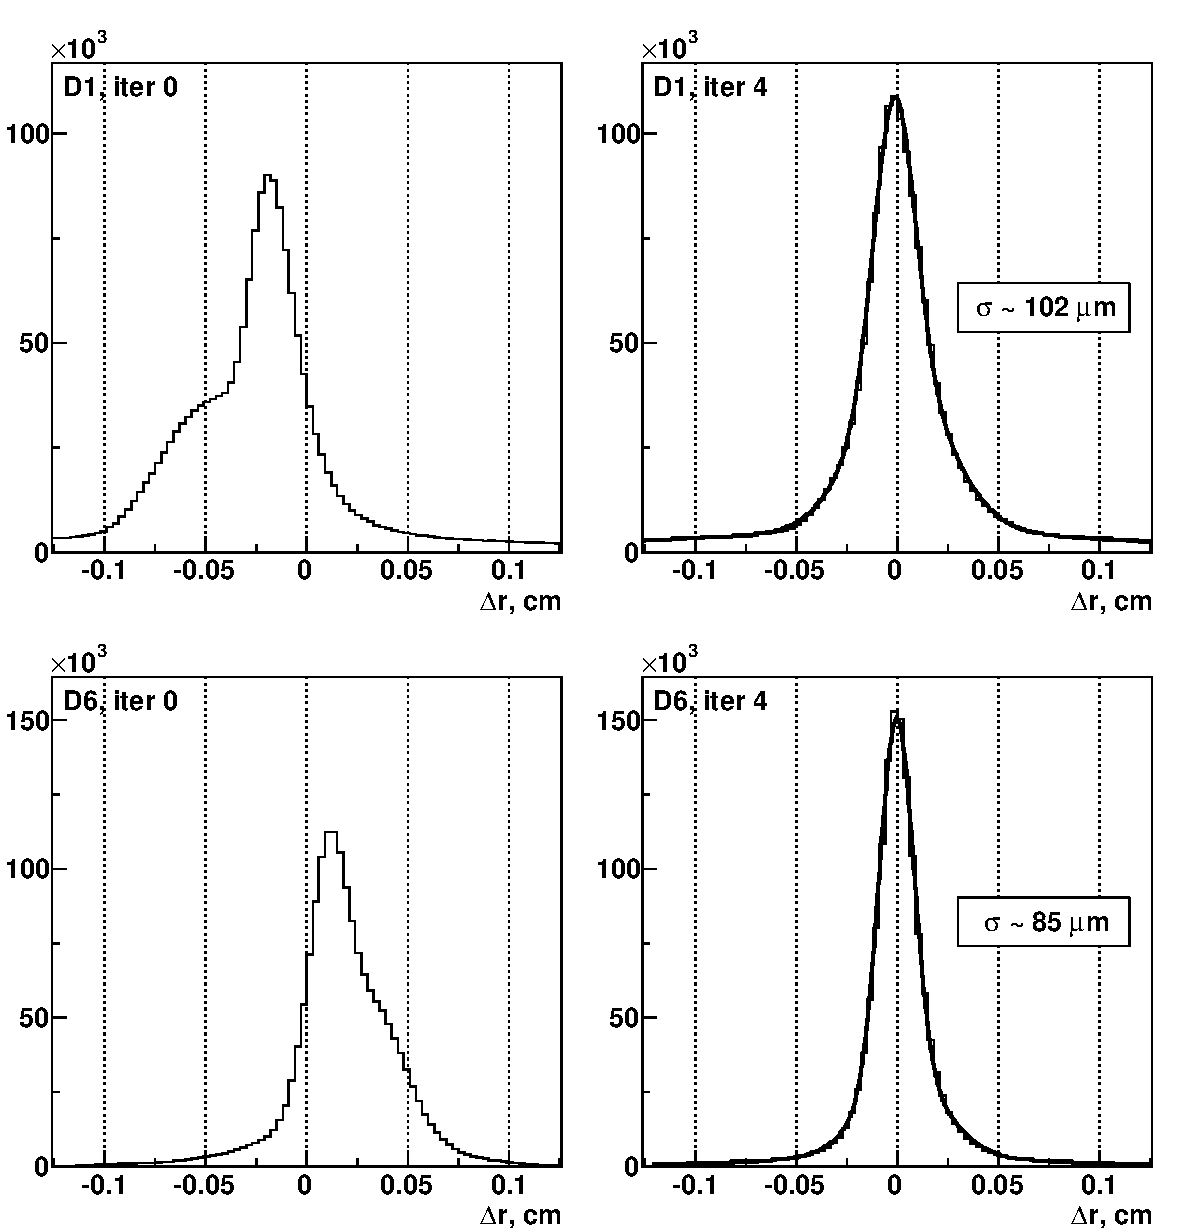
\includegraphics[width=1.00\textwidth]{res_chambers.pdf}
  \caption{Распределения трекового остатка $\triangle r$ в $xz$-плоскости
    дрейфовой камеры D1 и камеры D6. Слева~--- распределения с исходным
    интегральным $r(t)$-отношением, справа~--- после финальной четвёртой
    итерации автокалибровки, аппроксимированные двойным распределением Гаусса.}
  \label{fig:res_chambers}
\end{figure}

\section{Выводы к четвёртой главе}
Из проведённого в этой главе анализа можно сформулировать основные результаты:
\begin{list}{\labelitemi}{\leftmargin=1em}
\item В процессе создания и усовершенствования установки СТРЕЛА был разработан
  и реализован полный комплекс программ обработки и анализа экспериментальных
  данных.
\item Разработаны и протестированы на реальных событиях алгоритмы для поиска и
  реконструкции треков в дрейфовых камерах. Исходный код программ написан
  полностью на языке С++ с использованием библиотек ROOT, что делает их
  универсальными и модульными.
\item Показано, что созданная итеративная процедура автокалибровки существенно
  улучшает величину пространственного разрешения камер, среднее значение которой
  лежит в диапазоне 90--120~мкм.
\item Полученные характеристики трековых детекторов позволяют осуществить
  исследования зарядово-обменных процессов в дейтрон-протонных взаимодействиях
  на установке СТРЕЛА.
\item Созданная нами методика реконструкции событий после небольших изменений
  может быть использована и для других экспериментов, где применяются
  координатные детекторы, такие как дрейфовые камеры или трубки.
\end{list}

%%% Local Variables:
%%% mode: latex
%%% TeX-master: "musinsky_disser"
%%% coding: utf-8
%%% End:

\conclusion
Основные результаты исследований, проведённых в диссертации, можно
сформулировать следующим образом:
\begin{list}{\labelitemi}{\leftmargin=1em}
\item Проведён полный анализ $dp$-взаимодействий, полученных с помощью
  100-сантиметровой водородной пузырьковой камеры ЛВЭ ОИЯИ при импульсе
  3.35~ГэВ/с. Оценены потери в упругом рассеянии и получены значения поперечных
  сечений отдельных каналов $dp$-взаимодей\-ствий. Качество полученной
  экспериментальной информации свидетельствует о её пригодности для последующего
  физического анализа.

  \vspace{1ex}
  Впервые в эксклюзивной постановке исследована безмезонная реакция \dpfrag.
  Определено дифференциальное сечение реакции перезарядки
  $(d\sigma/dt)_{\dpchex}\,|\,_{t=0} = 30.2 \pm 4.1$~мб/(ГэВ/с)$^{2}$.

  \vspace{1ex}
  Впервые в пучке дейтронов получено отношение $R_{\np}$ дифференциальных
  сечений перезарядки при $t=0$ в реакции \dpchex и \np. В рамках импульсного
  приближения полученное значение $R_{\np} = 0.55\,\pm\,0.08$ свидетельствует о
  преобладающем вкладе спин-зависящей части сечения \np рассеяния и согласуется
  с данными других экспериментов в области близких энергий.

\item На основе результатов исследований с помощью водородной пузырьковой камеры
  был предложен электронный эксперимент для изучения реакции перезарядки на
  дейтроне в области энергий выше 1~ГэВ. Рассмотрена возможность определения
  спин-зависящей части амплитуды элементарной перезарядки \np на основе прямого
  измерения дифференциального сечения $(d\sigma/dt)_{\dpchex}$ при $t=0$.

  \vspace{1ex}
  При активном участии диссертанта была создана установка СТРЕЛА, основными
  элементами которой являются блоки дрейфовых камер. Впервые проведено
  облучение установки в пучке дейтронов импульса 3.5~ГэВ/с на ускорительном
  комплексе Нуклотрона ЛФВЭ ОИЯИ. Использование быстрой современной электроники
  повышает эффективность набора данных.

  \vspace{1ex}
  В процессе создания и усовершенствования установки СТРЕЛА были разработаны и
  реализованы комплексы программ обработки и анализа экспериментальных
  данных. Полученное значение пространственного разрешения дрейфовых
  камер лежит в диапазоне 90--120~мкм, что позволяет осуществить исследования
  зарядово-обменных процессов во взаимодействиях дейтронов с протонами.
\end{list}

\vfill
Работа выполнена в Лаборатории физики высоких энергий ОИЯИ им.~В.И.~Векслера и
А.М.~Балдина. Автор выражает благодарность дирекции лаборатории за
предоставленную возможность проведения исследований.
Автор считает своим приятным долгом выразить глубокую благодарность научному
руководителю В.В.~Глаголеву за постановку темы диссертационной работы, за особо
внимательное отношение к моей работе на всех её этапах и многочисленные ценные
дискуссии и советы. Искренне благодарен Г.~Мартинской и Н.М.~Пискунову за
большое внимание к выполненной работе, за многократные научные обсуждения
вопросов, за поправки и конструктивную критику. Автор выражает благодарность за
обсуждение теоретических вопросов Н.Б.~Ладыгиной.

Я признателен сотрудникам лаборатории, оказавшим помощь и всестороннюю поддержку
в сотрудничестве с которыми выполнена эта работа: С.Н.~Базылеву, Ю.П.~Бушуеву,
Д.А.~Кириллову, А.А.~Повторейко, В.М.~Слепнёву и И.В.~Слепнёву.
Автор глубоко признателен всем, чья помощь и поддержка сделала возможным
появления данного труда.

%%% Local Variables:
%%% mode: latex
%%% TeX-master: "musinsky_disser"
%%% coding: utf-8
%%% End:

\small
\def\BibEmph#1{\emph{#1}}
\bibliography{references}
\bibliographystyle{gost705}
\end{document}

%%% Local Variables:
%%% mode: latex
%%% TeX-master: t
%%% coding: utf-8
%%% End:
